% Created 2015-11-16 Mon 18:30
\documentclass{article}
\usepackage[top=1in, bottom=1.in, left=1in, right=1in]{geometry}
  \usepackage[makeroom]{cancel}
\usepackage{verbatim}


\usepackage[utf8]{inputenc}
\usepackage{lmodern}
\usepackage[T1]{fontenc}
\usepackage{fixltx2e}
\usepackage{graphicx}
\usepackage{longtable}
\usepackage{float}
\usepackage{wrapfig}
\usepackage{rotating}
\usepackage[normalem]{ulem}
\usepackage{amsmath}
\usepackage{textcomp}
\usepackage{marvosym}
\usepackage{wasysym}
\usepackage{amssymb}
\usepackage{amsmath}
\usepackage[version=3]{mhchem}
\usepackage[numbers,super,sort&compress]{natbib}
\usepackage{natmove}
\usepackage{url}
\usepackage{minted}
\usepackage{underscore}
\usepackage[linktocpage,pdfstartview=FitH,colorlinks,
linkcolor=blue,anchorcolor=blue,
citecolor=blue,filecolor=blue,menucolor=blue,urlcolor=blue]{hyperref}
\usepackage{attachfile}
\author{Abhishek Bagusetty}
\date{\today}
\title{24-623 2015 HM5}
\begin{document}

\maketitle

\section{Problem 1}
\label{sec-1}
Integration is performed with the random sampling monte-carlo integration of the variables. 
Program is evaluated at different sample sizes and the averages are reported for an average of 5 runs. Plots are shown for the value of PI and the error estimates at different sample sizes in Figures. \ref{fig:P1a} and \ref{fig:P1b}.

\begin{figure}[htb]
\centering
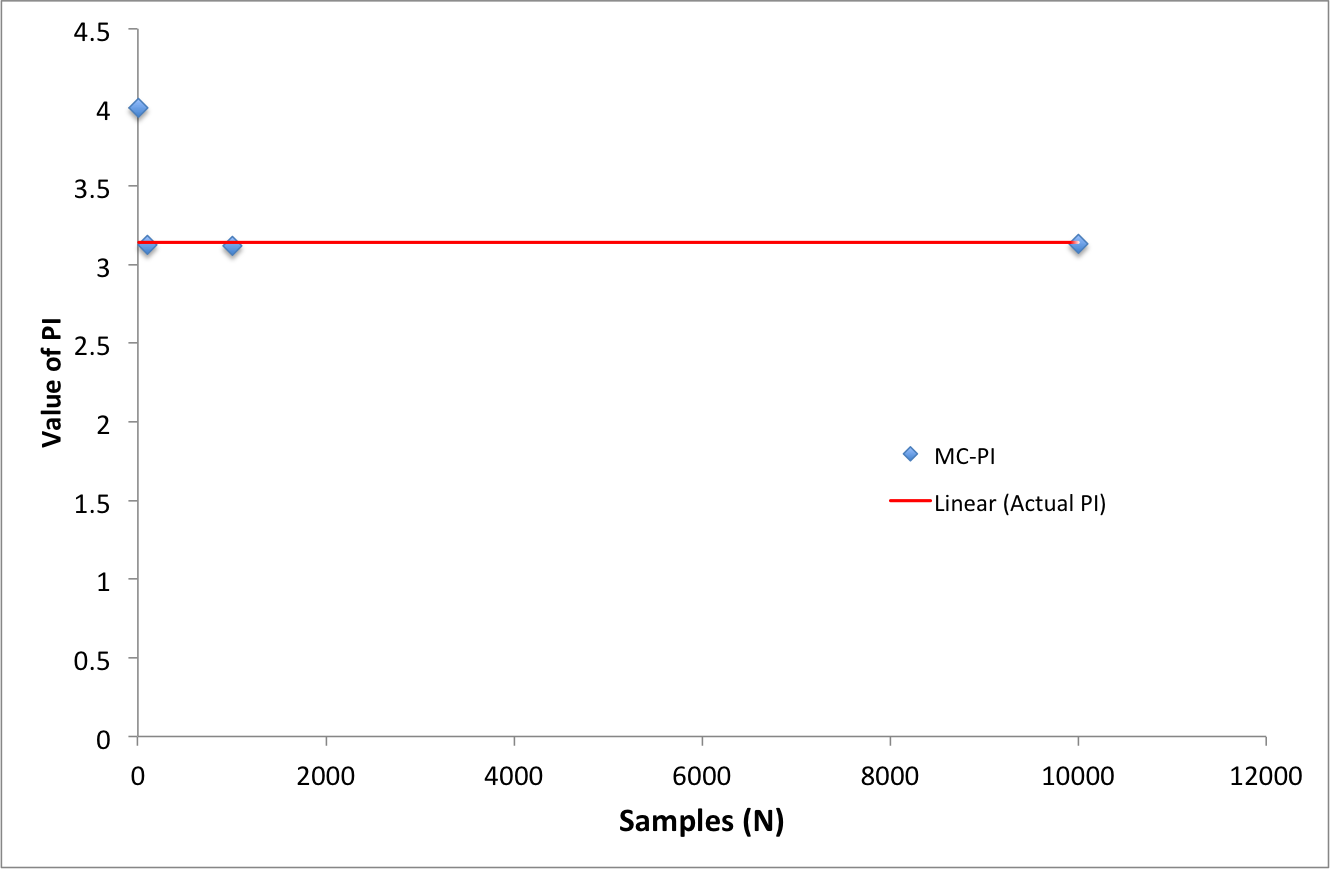
\includegraphics[width=.9\linewidth]{./P1/PI.png}
\caption{\label{fig:P1a}The figure shows the value of PI at different sample sizes computed from the random sampling monte-carlo integration.}
\end{figure}

\begin{figure}[htb]
\centering
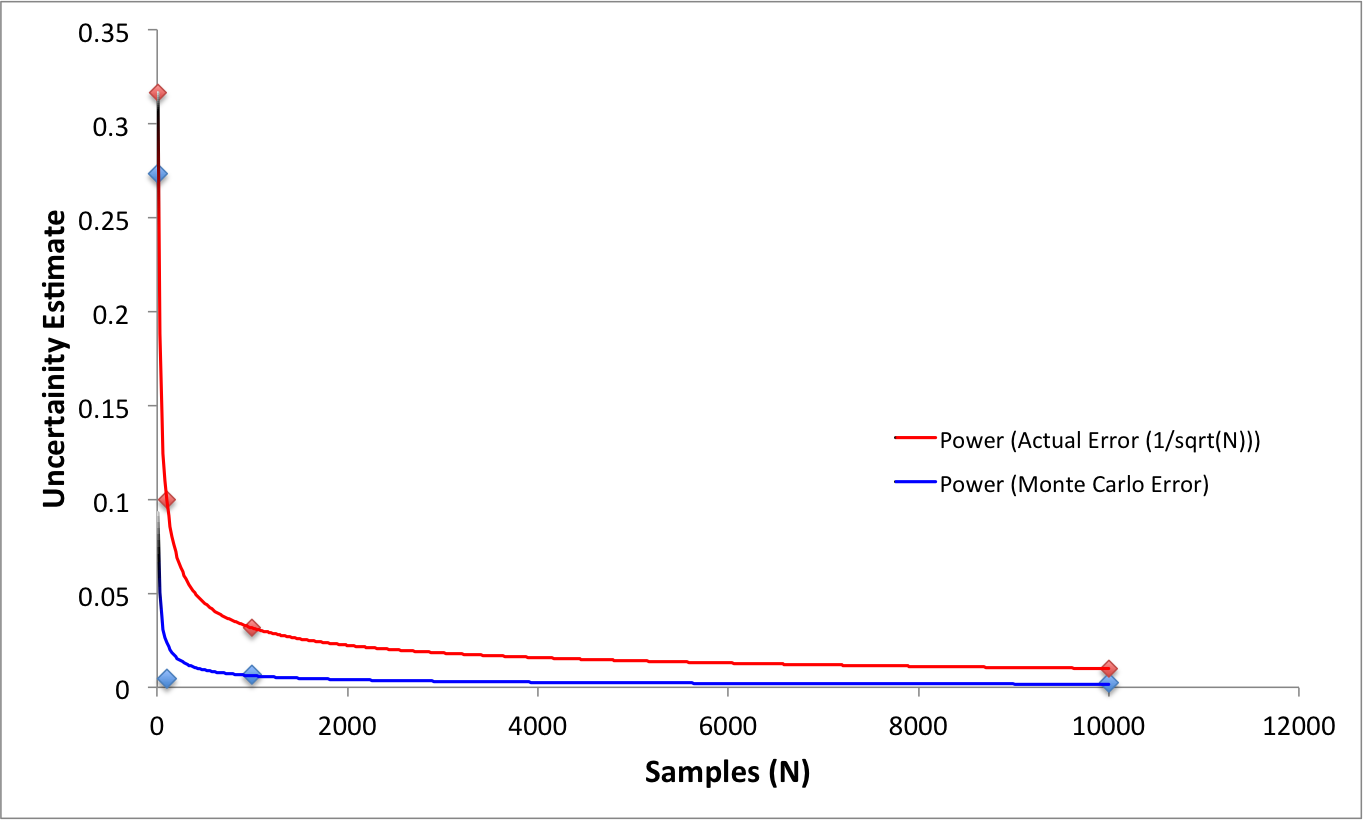
\includegraphics[width=.9\linewidth]{./P1/Error-Estimate.png}
\caption{\label{fig:P1b}The figure shows the error estimates for the value of PI. The relative error is plotted against the sample sizes to show the convergence of the error with respect to the sample sizes. The actual error estimate varies according to the red curve.}
\end{figure}

The uncertainity for the computation of PI is estimated using relative error $(Q_{N}-\pi)/\pi$, where $Q_{N}$ is the value of the PI obtained from the monte-carlo integration. The relative error is expected to change with the samples(N) according to the order, $\mathscr{O(1/ \sqrt N)}$

The number of samples required for obtaining an accuracy till 20 significant digits is obtained from the relation $$ \frac{1}{\sqrt{N}} \propto \frac{Q_{N}-\pi}{\pi}$$

The absolute error will be in the order of 1.0e-21 for 20 significant digits accuracy.
\begin{equation}
\frac{1}{\sqrt{N}} \propto \frac{1.0e-21}{3.142857......(20 digits)}
\label{eq:1}
\end{equation}

\begin{equation}
N \propto \frac{1}{(3.18309e-22)^2}
\label{eq:2}
\end{equation}

Hence to achieve an accuracy of 20 significant digits from the Monte Carlo integration one would require, N = 1.0e+43 samples, computed from Eq.\ref{eq:1}.

\section{Problem 2}
\label{sec-2}
\subsection{a)}
\label{sec-2-1}

The values of $\langle U \rangle, \langle x \rangle, \langle x^2 \rangle$ are computed analytically and they are reported for harmonic oscillator a) $U(x) = x^2/2$.

\begin{equation}
\langle U \rangle = \frac{\int_{-\infty}^{\infty} U(x) exp(-\beta U(x))}{\int_{-\infty}^{\infty} exp(-\beta U(x))}
\label{eq:P2a}
\end{equation}
\begin{equation}
\langle x \rangle = \frac{\int_{-\infty}^{\infty} x exp(-\beta U(x))}{\int_{-\infty}^{\infty} exp(-\beta U(x))}
\label{eq:P2b}
\end{equation}
\begin{equation}
\langle x^2 \rangle = \frac{\int_{-\infty}^{\infty} x^2 exp(-\beta U(x))}{\int_{-\infty}^{\infty} exp(-\beta U(x))}
\label{eq:P2c}
\end{equation}

The average values are shown below :

\begin{table}[htb]
\caption{\label{tab:table1}Values of \langle U \rangle, \langle x \rangle, \langle x$^{\text{2}}$ \rangle,  are tabulated below computed from analytical expressions.}
\centering
\begin{tabular}{rrrr}
\hline
$\beta$ & \langle U \rangle & \langle x \rangle & \langle x$^{\text{2}}$ \rangle\\
\hline
0.1 & 5 & 0.0 & 10\\
1 & 0.4998 & 0.0 & 1.0\\
5 & 0.1 & 0.0 & 0.2\\
10 & 0.05 & 0.0 & 0.1\\
\hline
\end{tabular}
\end{table}

Using the Metropolis Monte Carlo technique, the percentage of acceptance with respect to the values of $\beta$ at different maximum step sizes is tabulated below \ref{tab:table2} : 

\begin{table}[htb]
\caption{\label{tab:table2}Percentage of acceptance of the moves with respect to various values of $\beta$ and  max. step sizes is shown below.}
\centering
\begin{tabular}{rrrrr}
\hline
$\delta$ dx$_{\text{max}}$ & $\beta$=0.1 & $\beta$=1 & $\beta$=5 & $\beta$=10\\
\hline
0.05 & 50.024 & 49.544 & 49.025 & 48.543\\
0.5 & 48.491 & 44.948 & 39.232 & 34.891\\
5 & 35.184 & 15.809 & 7.152 & 5.097\\
\hline
\end{tabular}
\end{table}

\textbf{PARAMTERS} : By looking at the Figs. \ref{fig:1a-01}, \ref{fig:1a-1}, \ref{fig:1a-5}, \ref{fig:1a-10}, the number of moves considered for this study is at 100,000. Better statistics could probably be obtained by using larger number of trail moves. The most important factor considered in this case is the value of step size. Different step size values are considered for every value of $\beta$=0.1,1,5,10 and the best value of step size is chosen based on acceptance percentage of the moves as shown in Table. \ref{tab:table2}. At the maximum step size of 0.5, the average value of the parameters oscillate about the standard value. Hence, a maximum step size of 0.5 is considered for data analysis. The following plots (Figs. \ref{fig:1a-01}, \ref{fig:1a-1}, \ref{fig:1a-5}, \ref{fig:1a-10}) gives the information. Running averages are plotted in Figs.  \ref{fig:1a-01}, \ref{fig:1a-1}, \ref{fig:1a-5}, \ref{fig:1a-10}.

\begin{figure}[!tbp]
  \centering
\subfloat{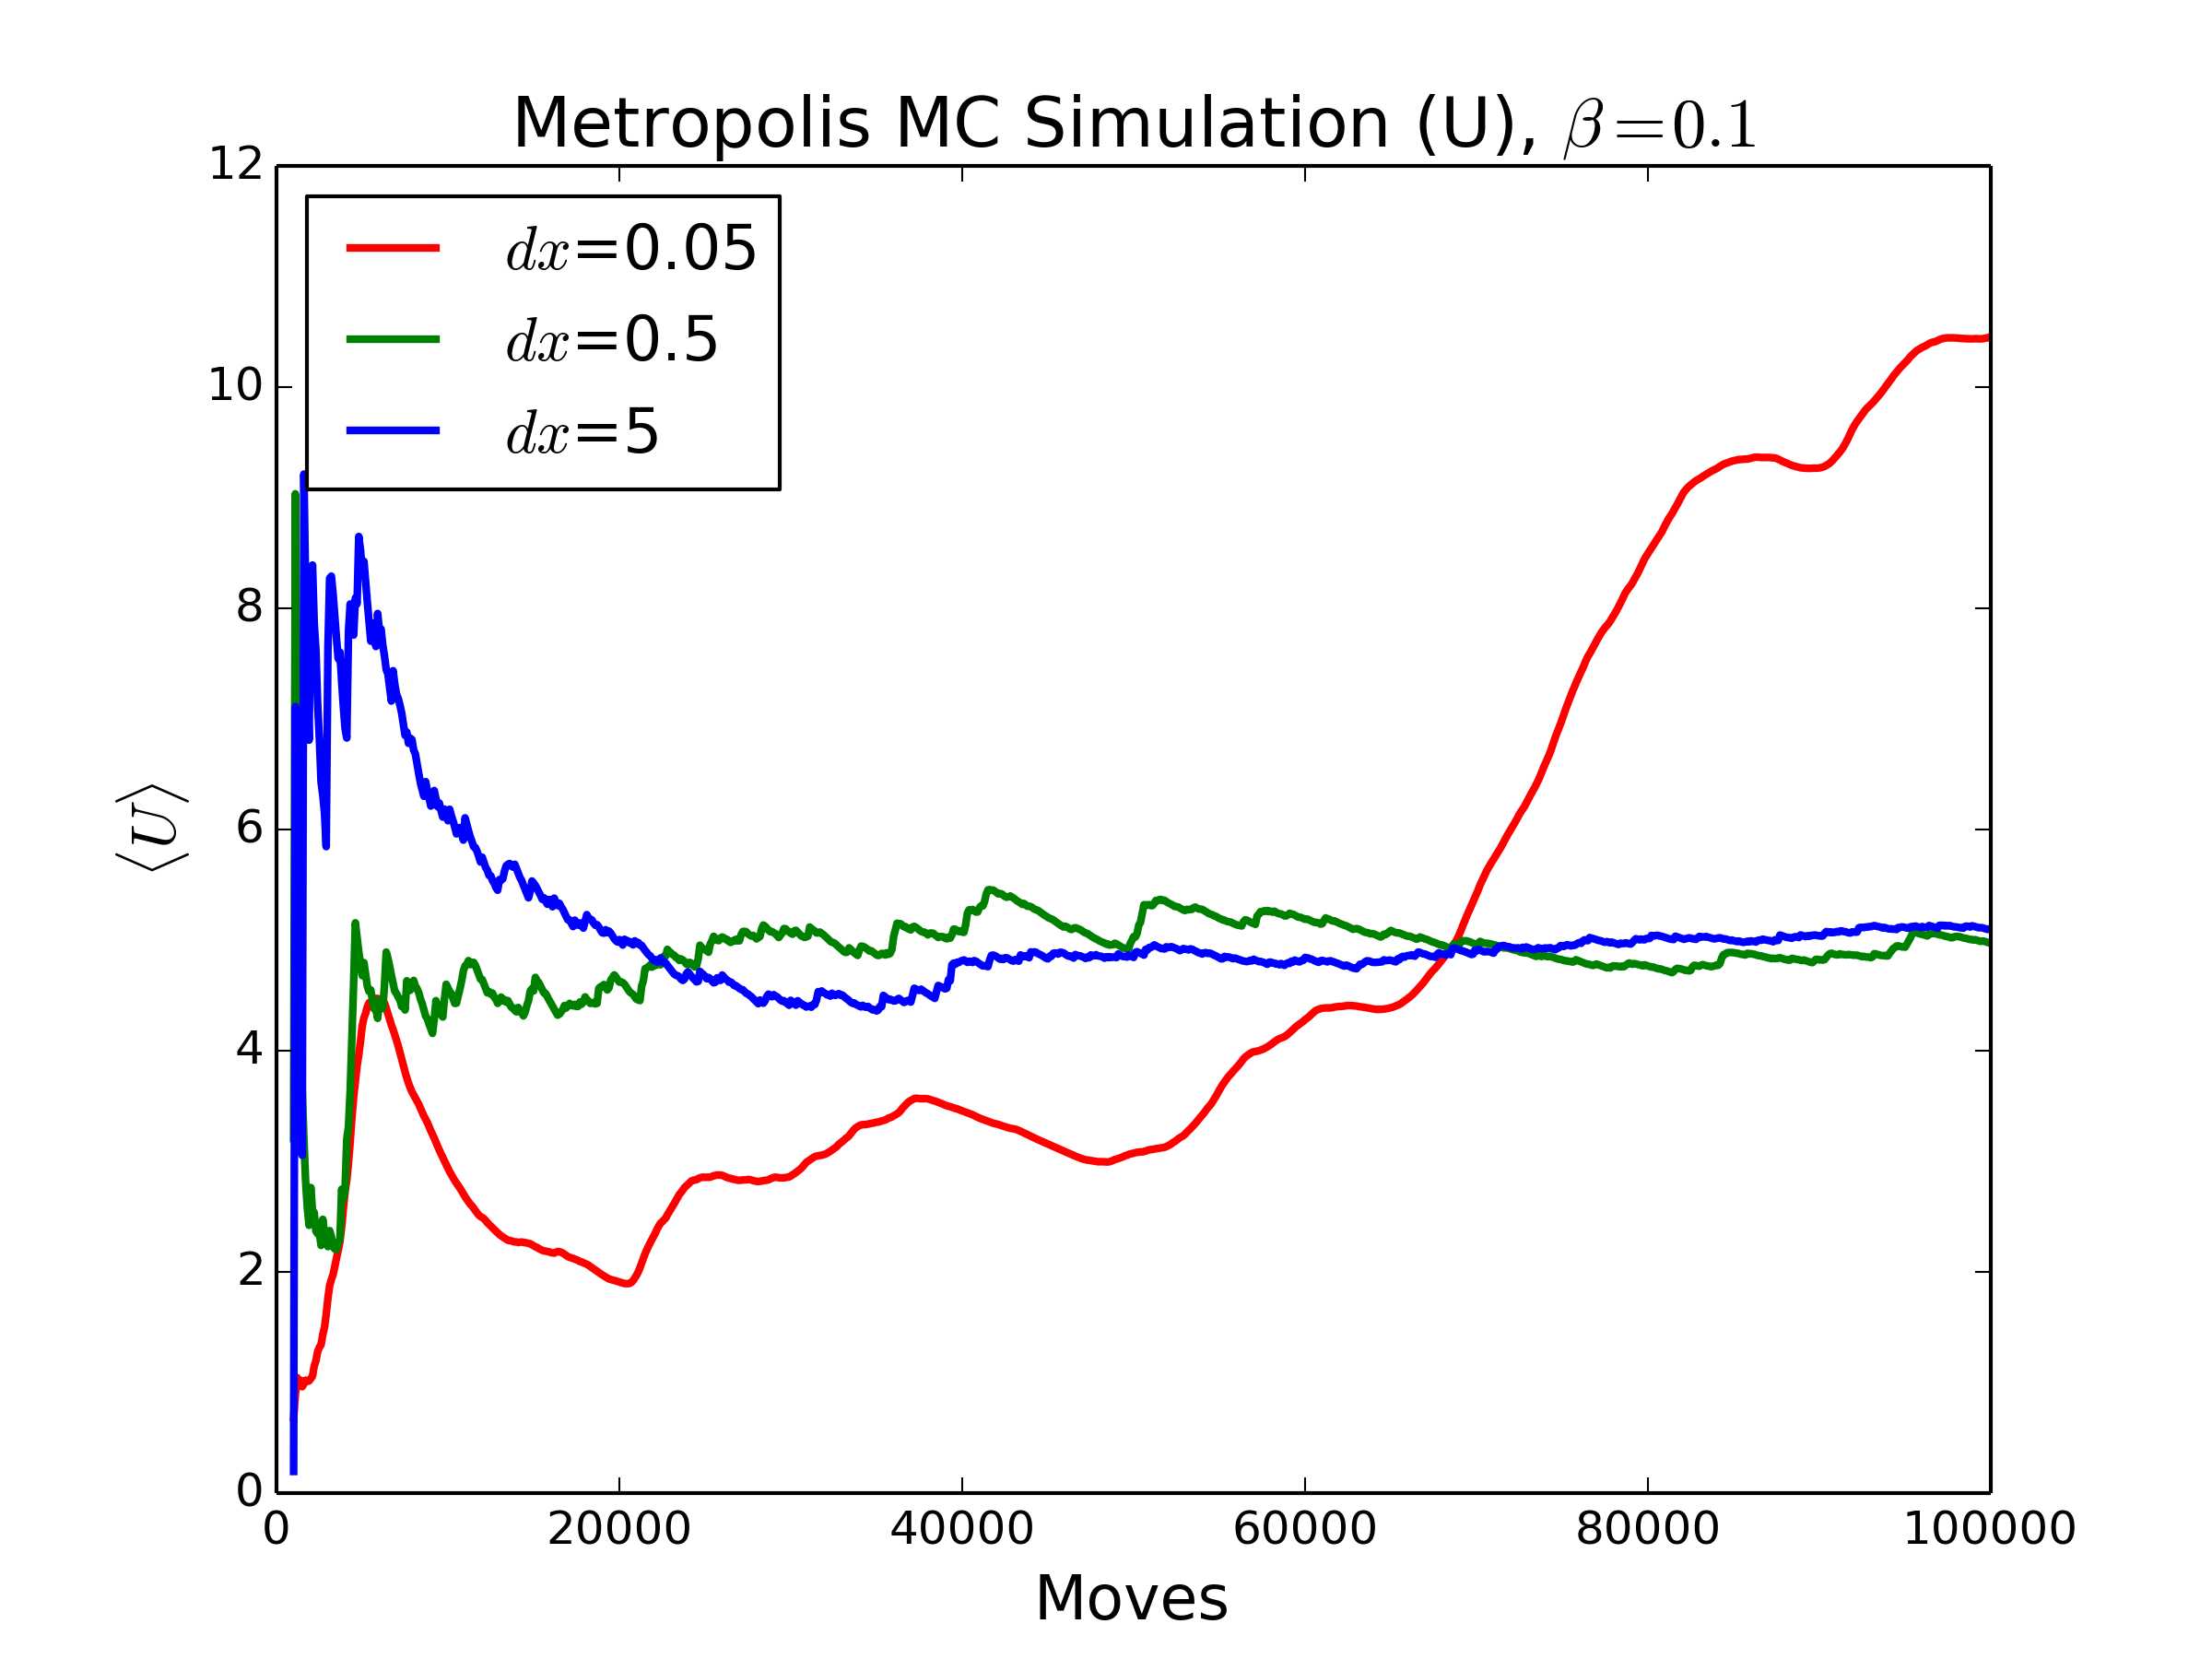
\includegraphics[width=0.49\textwidth]{./P2/part-a-beta-0.1/Oscillator2a-U.png}\label{fig:f1}}
  \hfill
\subfloat{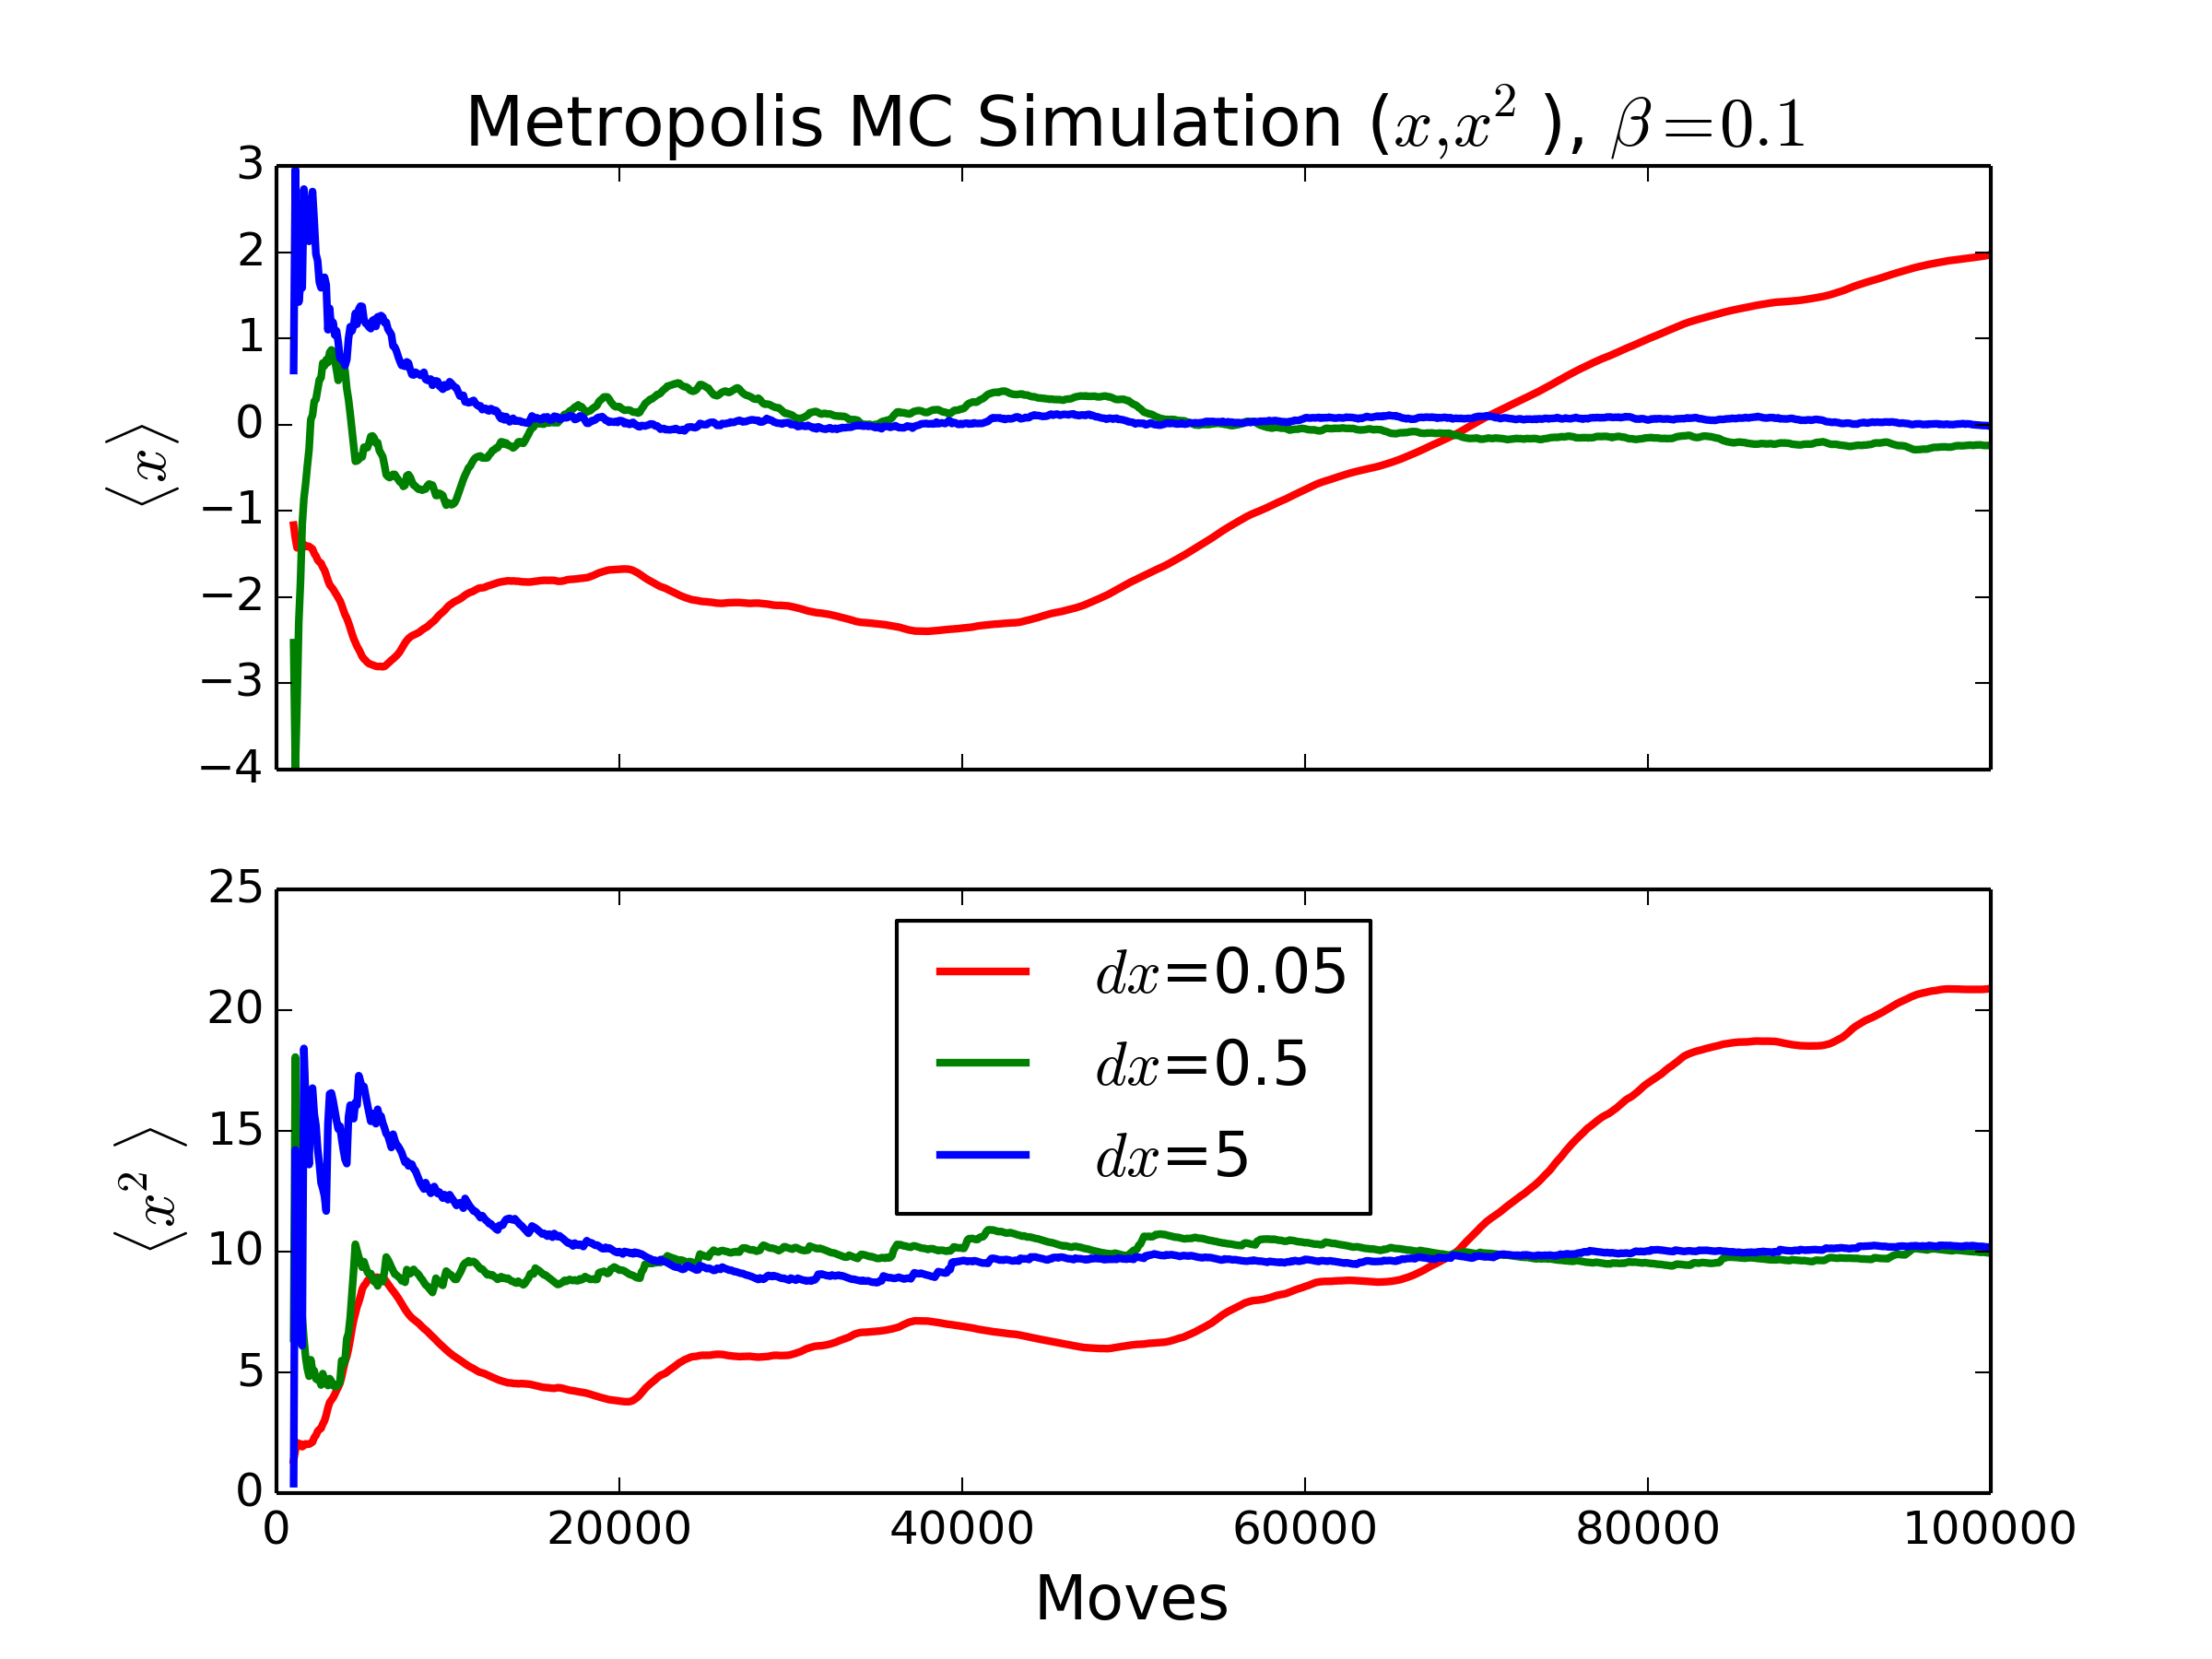
\includegraphics[width=0.49\textwidth]{./P2/part-a-beta-0.1/Oscillator2a-x.png}\label{fig:f1}}
  \caption{Monte Carlo Simulation of oscillator at \beta=0.1}
  \label{fig:1a-01}
\end{figure}

\begin{figure}[!tbp]
  \centering
\subfloat{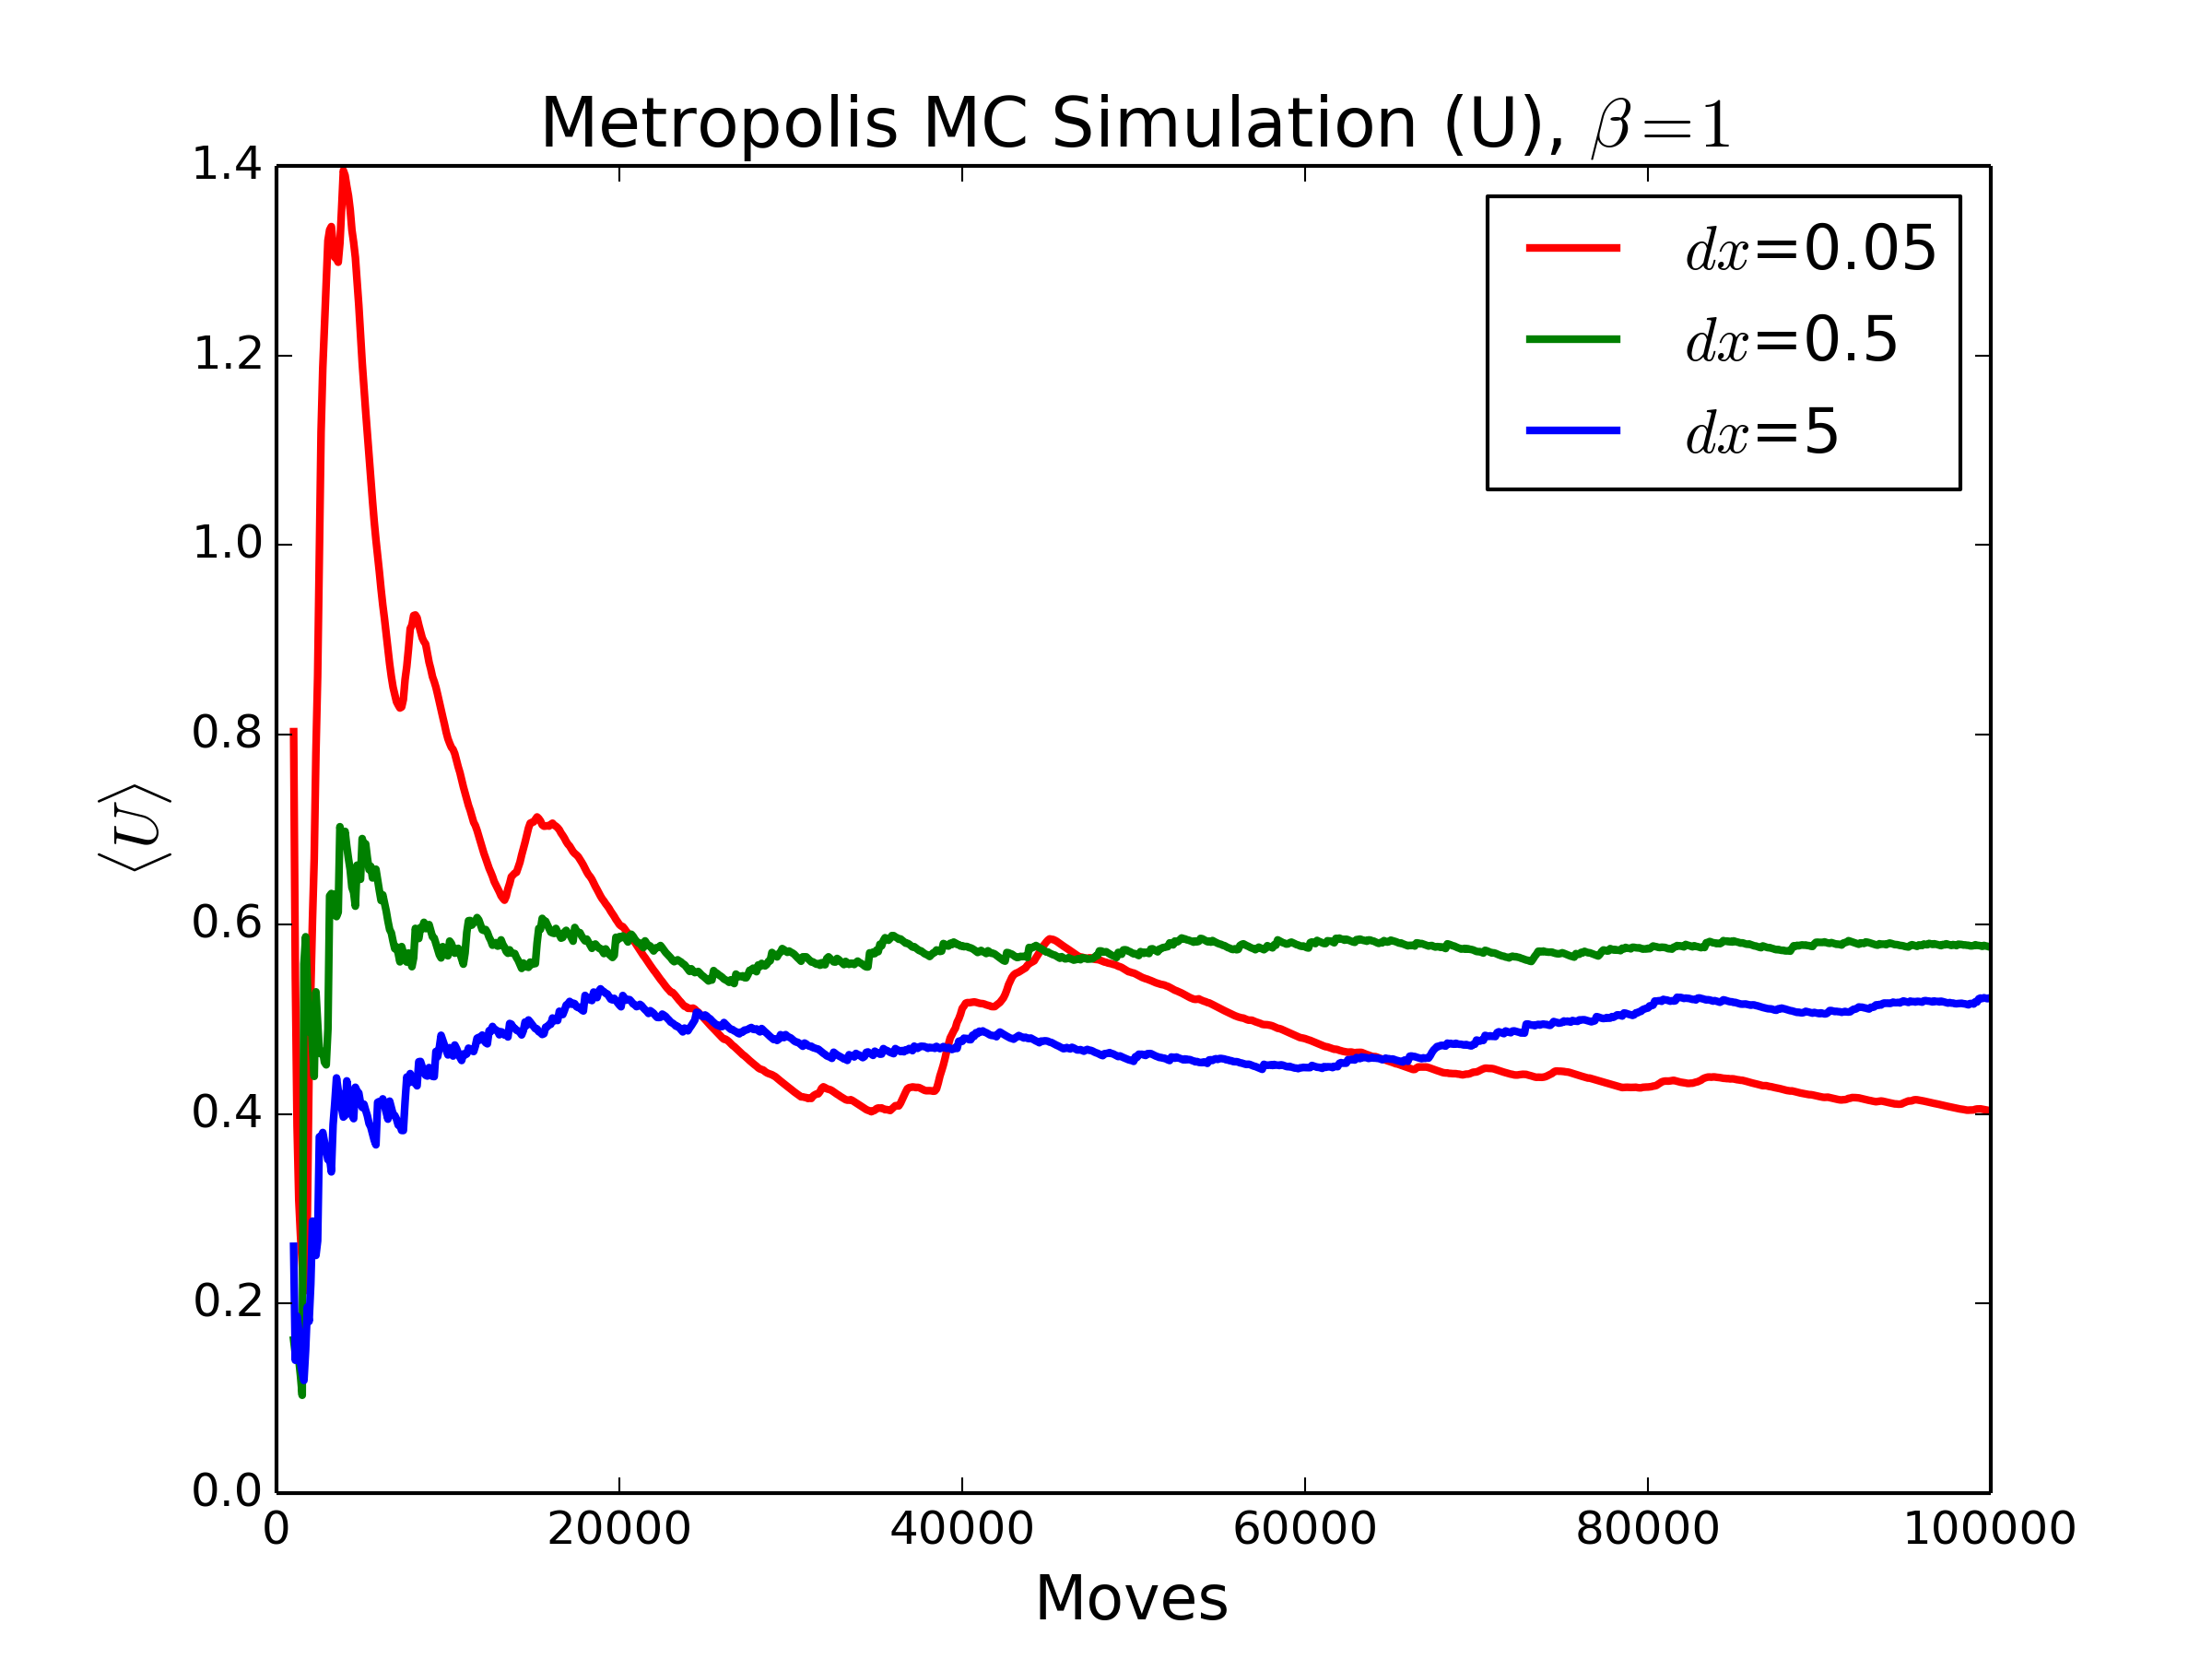
\includegraphics[width=0.49\textwidth]{./P2/part-a-beta-1/Oscillator2a-U.png}\label{fig:f1}}
  \hfill
\subfloat{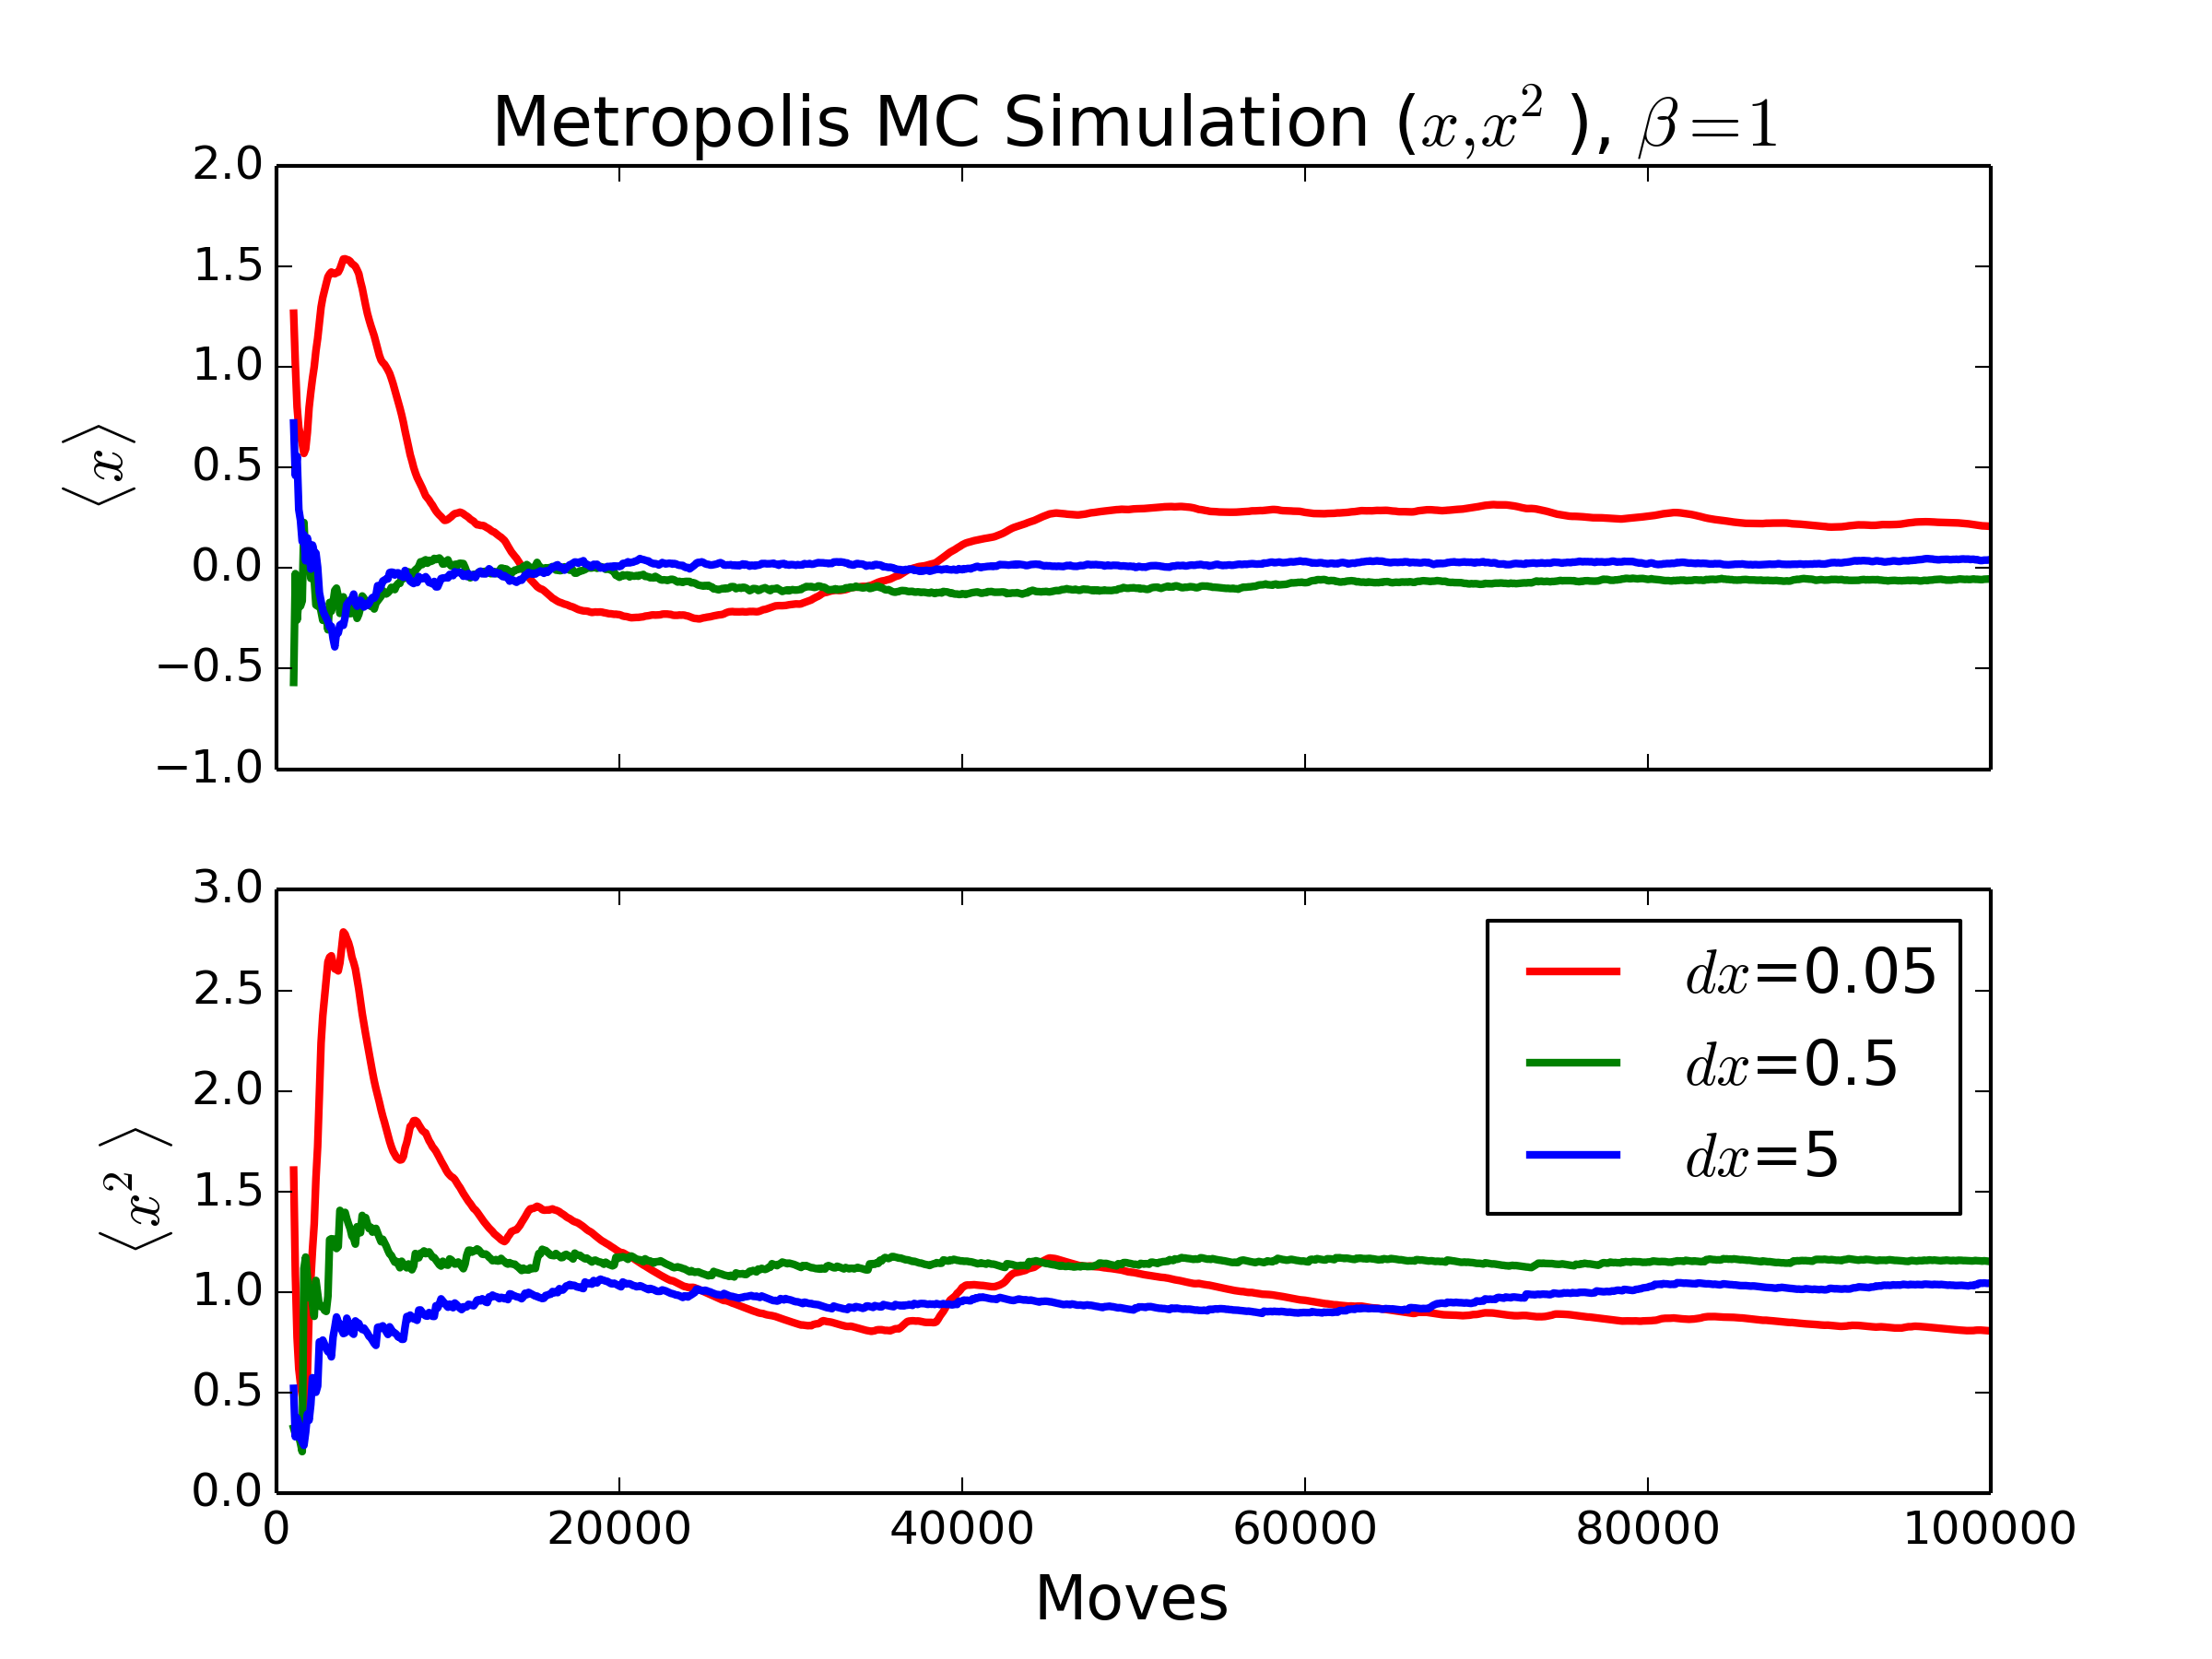
\includegraphics[width=0.49\textwidth]{./P2/part-a-beta-1/Oscillator2a-x.png}\label{fig:f1}}
  \caption{Monte Carlo Simulation of oscillator at \beta=1}
  \label{fig:1a-1}
\end{figure}

\begin{figure}[!tbp]
  \centering
\subfloat{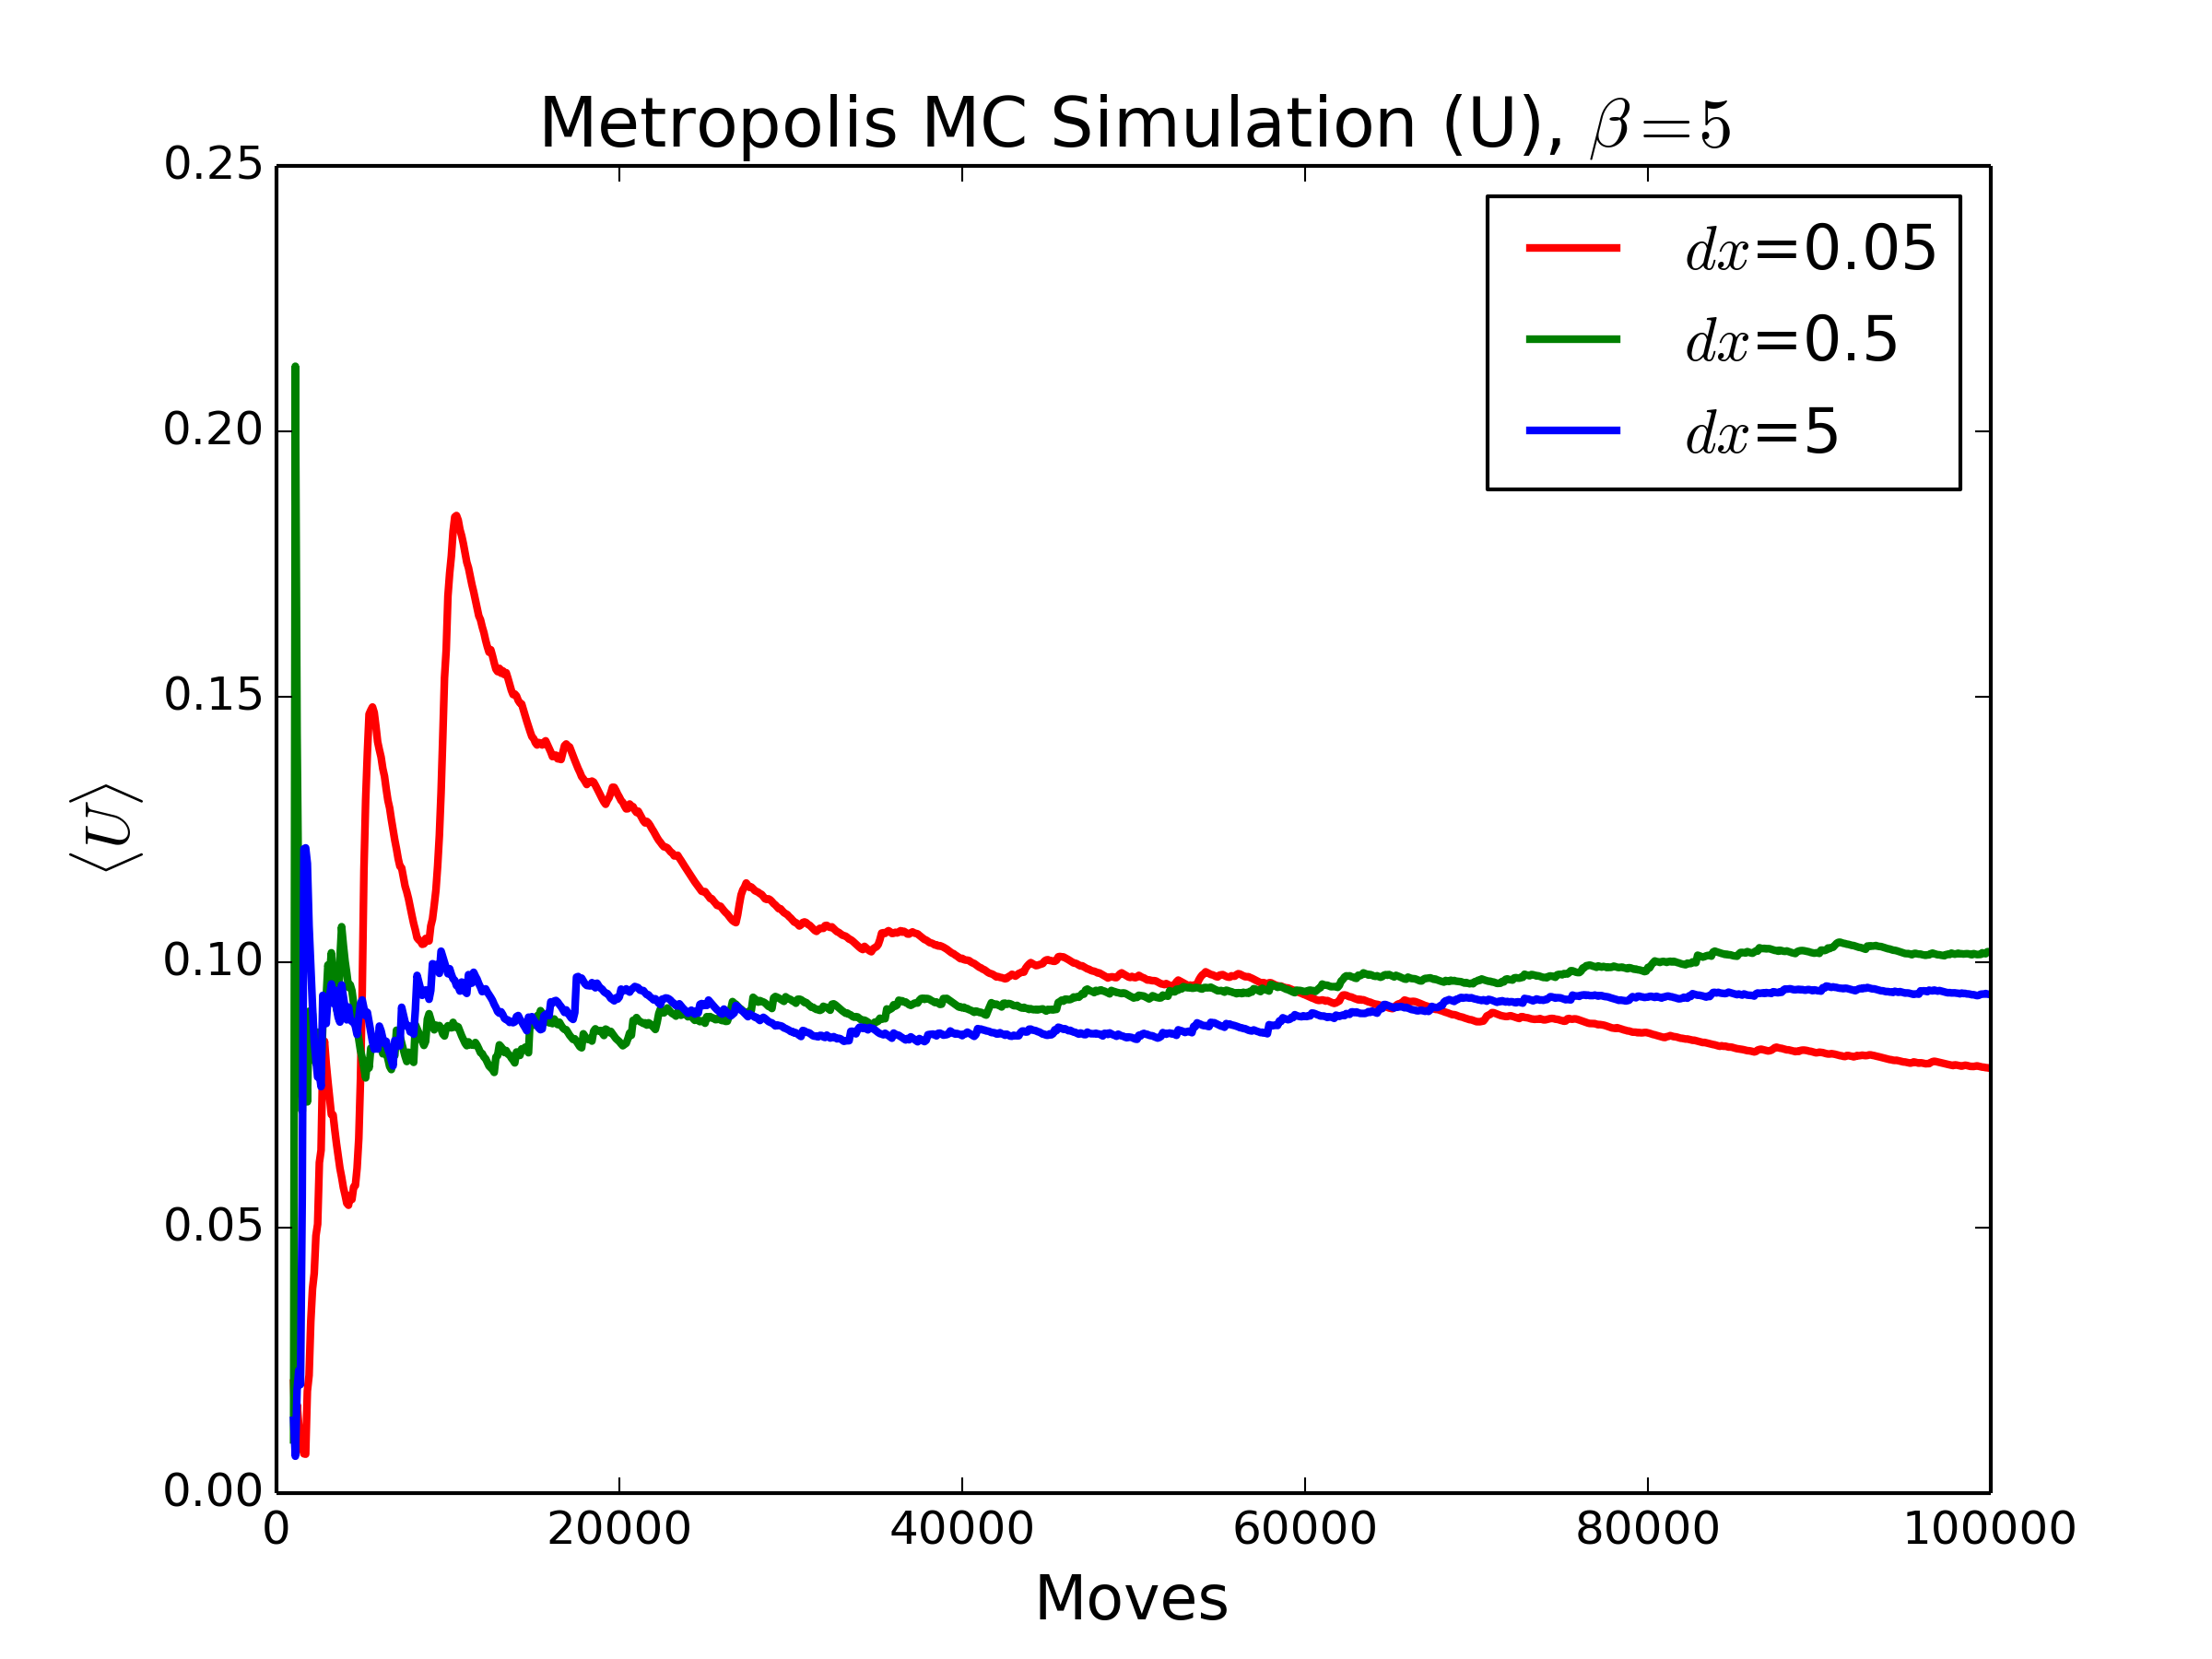
\includegraphics[width=0.49\textwidth]{./P2/part-a-beta-5/Oscillator2a-U.png}\label{fig:f1}}
  \hfill
\subfloat{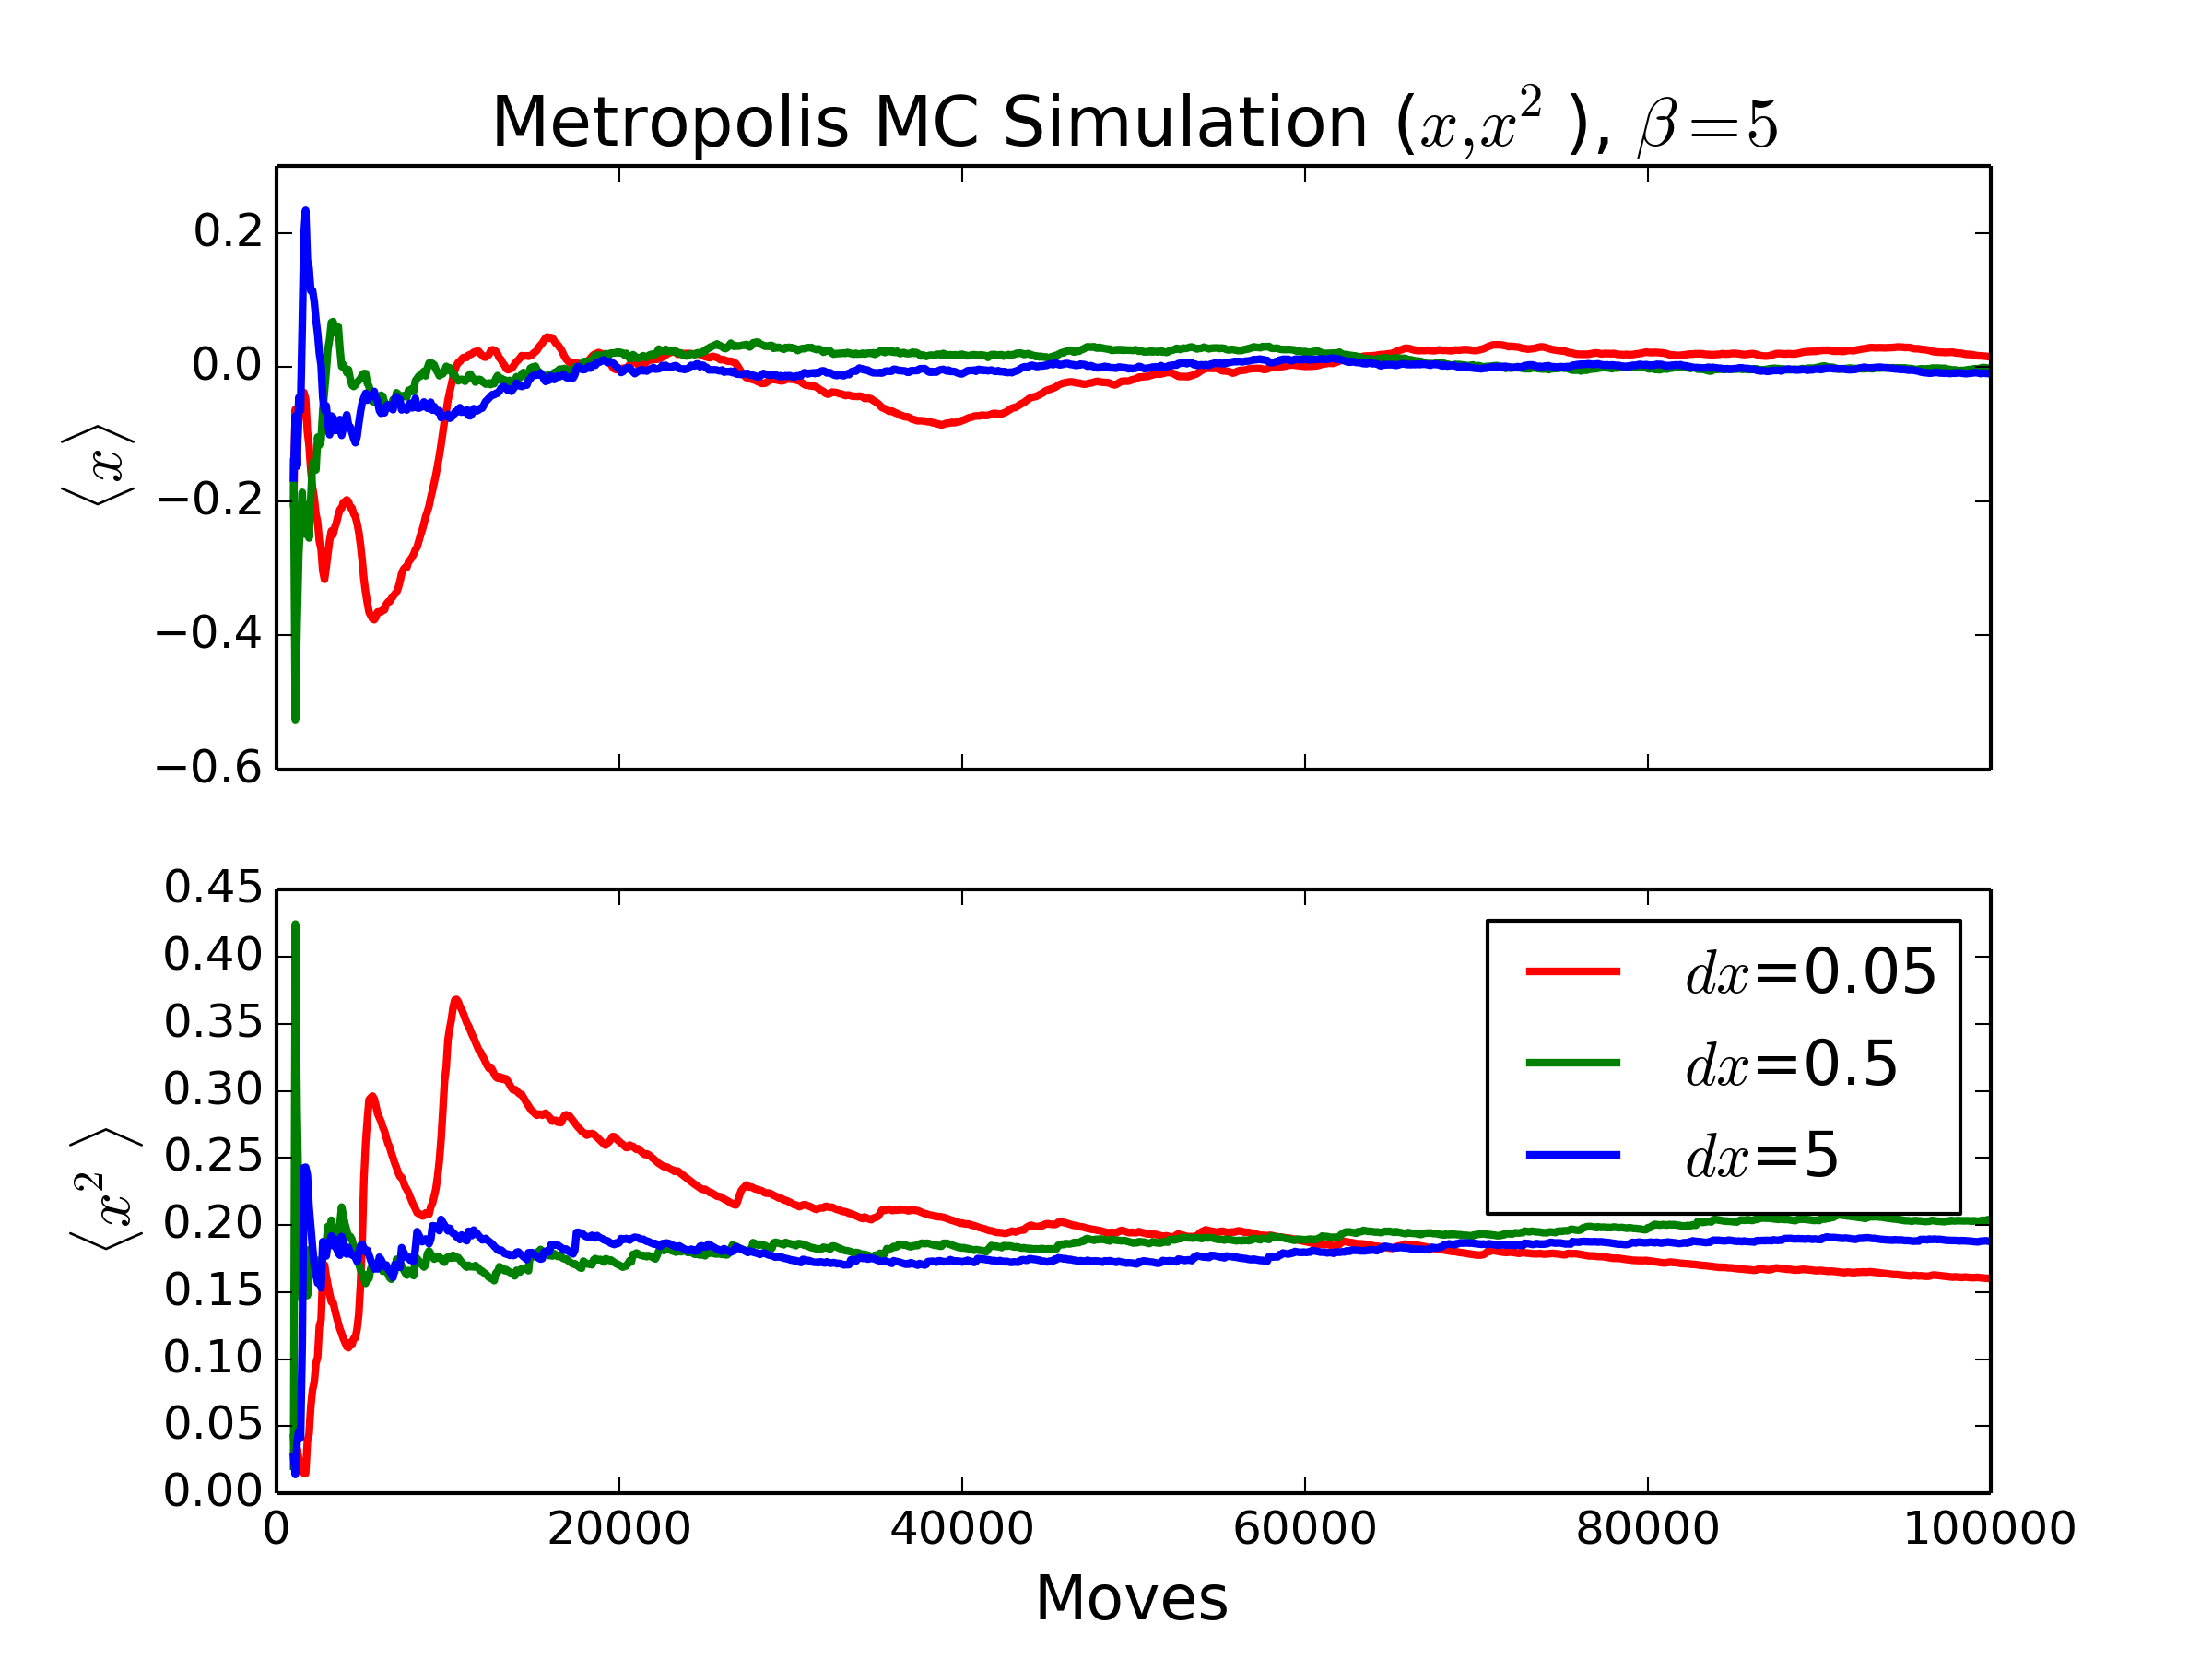
\includegraphics[width=0.49\textwidth]{./P2/part-a-beta-5/Oscillator2a-x.png}\label{fig:f1}}
  \caption{Monte Carlo Simulation of oscillator at \beta=5}
  \label{fig:1a-5}
\end{figure}

\begin{figure}[!tbp]
  \centering
\subfloat{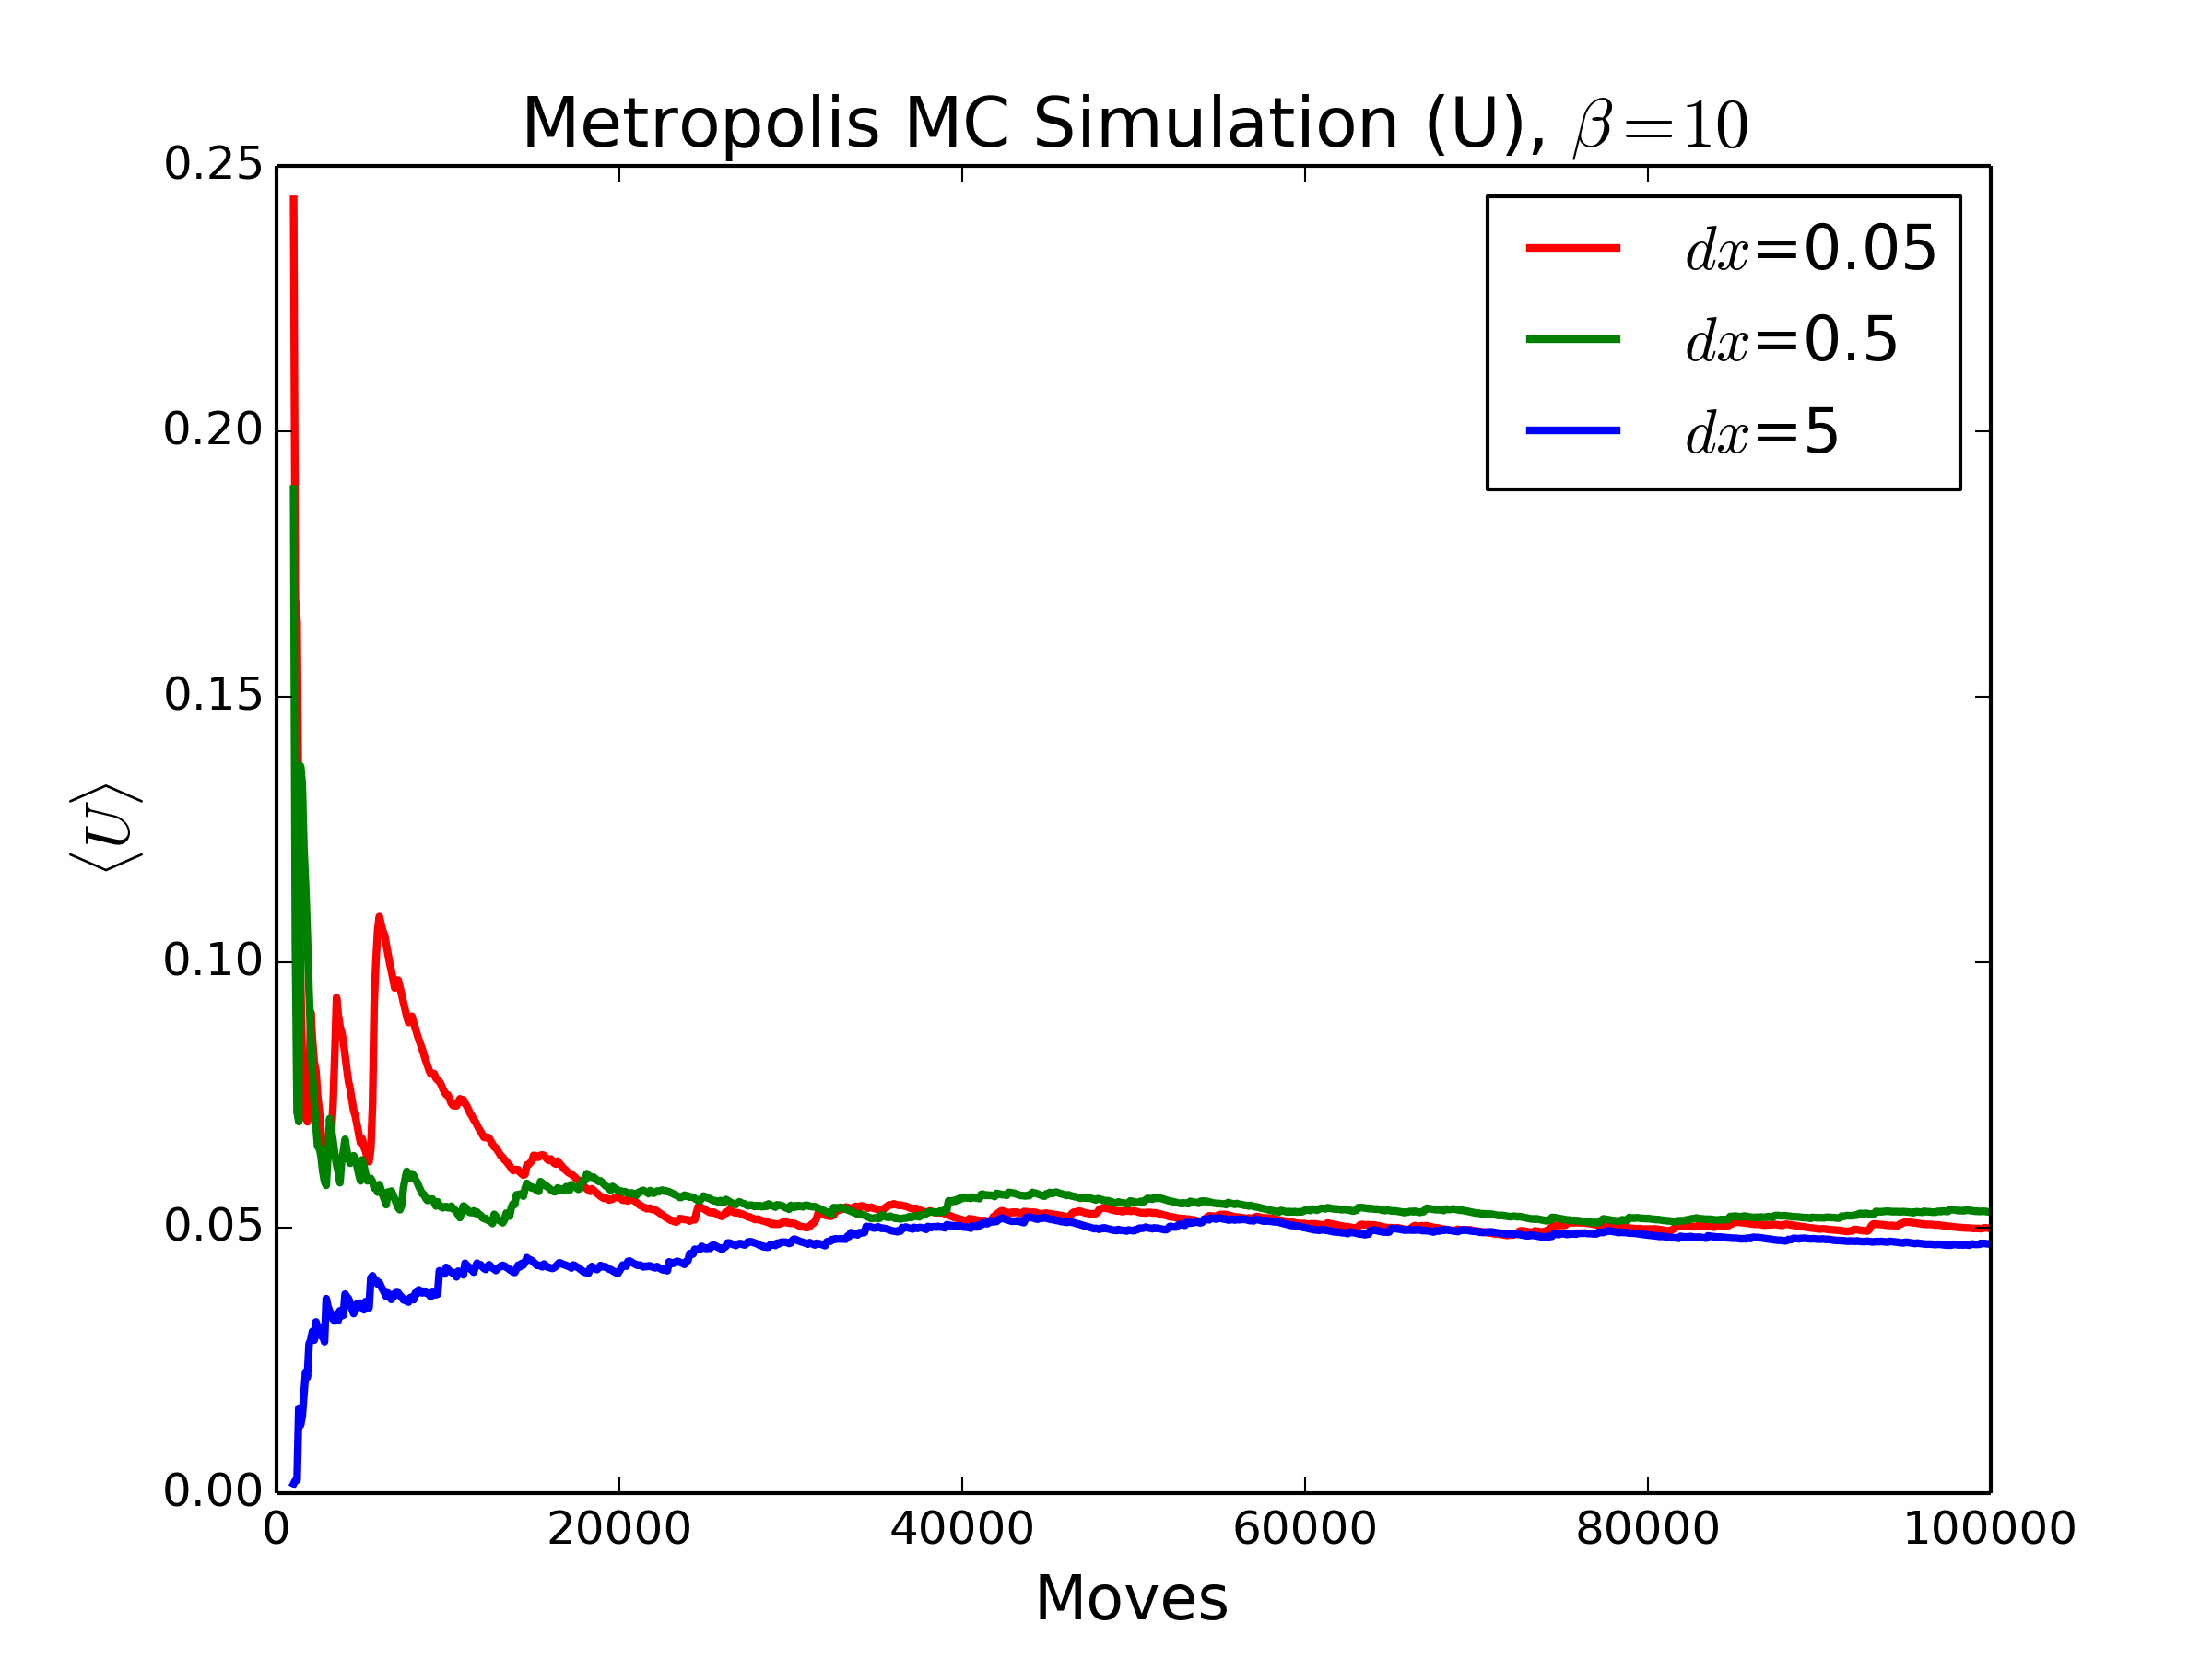
\includegraphics[width=0.49\textwidth]{./P2/part-a-beta-10/Oscillator2a-U.png}\label{fig:f1}}
  \hfill
\subfloat{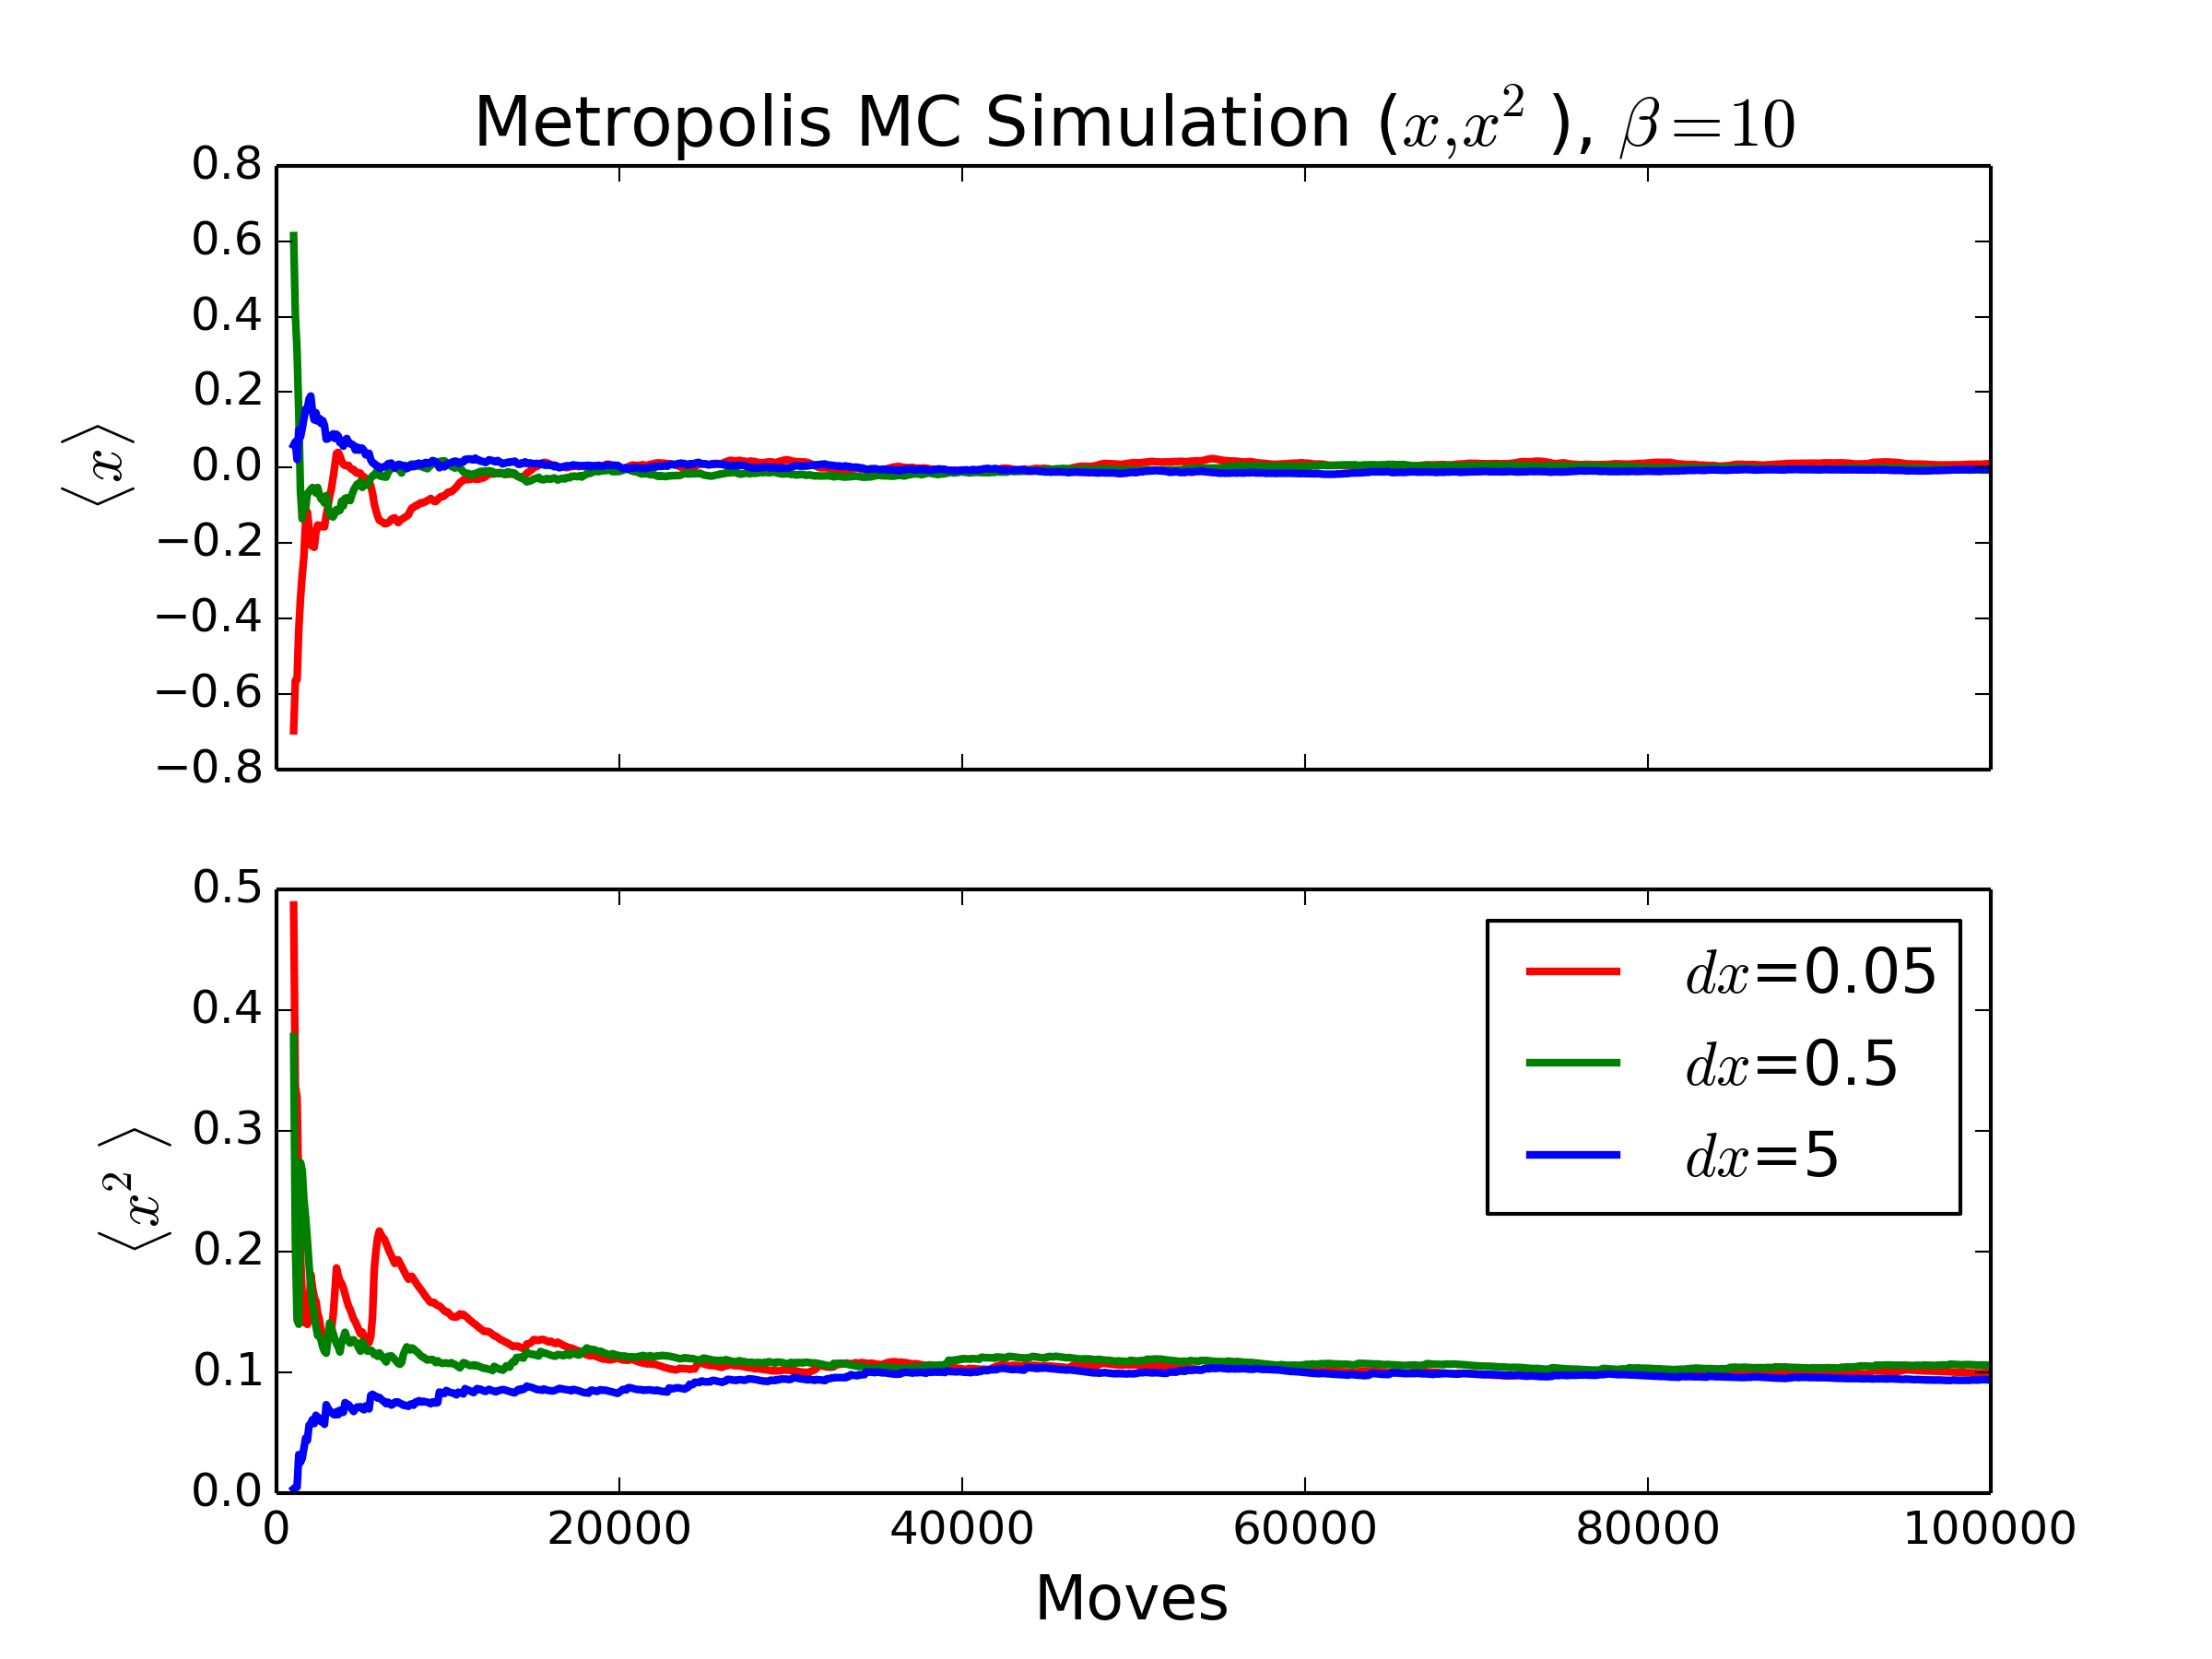
\includegraphics[width=0.49\textwidth]{./P2/part-a-beta-10/Oscillator2a-x.png}\label{fig:f1}}
  \caption{Monte Carlo Simulation of oscillator at \beta=10}
  \label{fig:1a-10}
\end{figure}

\subsection{b)}
\label{sec-2-2}
The values of $\langle U \rangle, \langle x \rangle, \langle x^2 \rangle$ are computed analytically for oscillator b) $U(x) = x^4-2x^2+1$. The average values are computed using Eqns. \ref{eq:P2a}, \ref{eq:P2b}, \ref{eq:P2c}

The average values are shown below in Table. \ref{tab:table3}:

\begin{table}[htb]
\caption{\label{tab:table3}Values of \langle U \rangle, \langle x \rangle, \langle x$^{\text{2}}$ \rangle are tabulated below computed from analytical expressions.}
\centering
\begin{tabular}{rrrr}
\hline
$\beta$ & \langle U \rangle & \langle x \rangle & \langle x$^{\text{2}}$ \rangle\\
\hline
0.1 & 2.1041757932 & 0.0 & 1.3958242068\\
1 & 0.417254512872 & 0.0 & 0.832745487128\\
5 & 0.113166059588 & 0.0 & 0.936833940412\\
10 & 0.0524772417986 & 0.0 & 0.972522758201\\
\hline
\end{tabular}
\end{table}

Using the Metropolis Monte Carlo technique, the percentage of acceptance with respect to the values of $\beta$ at different maximum step sizes is tabulated below \ref{tab:table2}. Running average of the parameters are also shown below in Figs. \ref{fig:1b-01}, \ref{fig:1b-1}, \ref{fig:1b-5}, \ref{fig:1b-10}

\begin{table}[htb]
\caption{\label{tab:table4}Percentage of acceptance of the moves with respect to various values of $\beta$ and max. step sizes is shown below.}
\centering
\begin{tabular}{rrrrr}
\hline
$\delta$ dx$_{\text{max}}$ & $\beta$=0.1 & $\beta$=1 & $\beta$=5 & $\beta$=10\\
\hline
0.05 & 49.722 & 48.696 & 46.986 & 45.614\\
0.5 & 46.299 & 40.189 & 25.116 & 18.07\\
5 & 19.853 & 12.223 & 5.476 & 3.931\\
\hline
\end{tabular}
\end{table}

\begin{figure}[!tbp]
  \centering
\subfloat{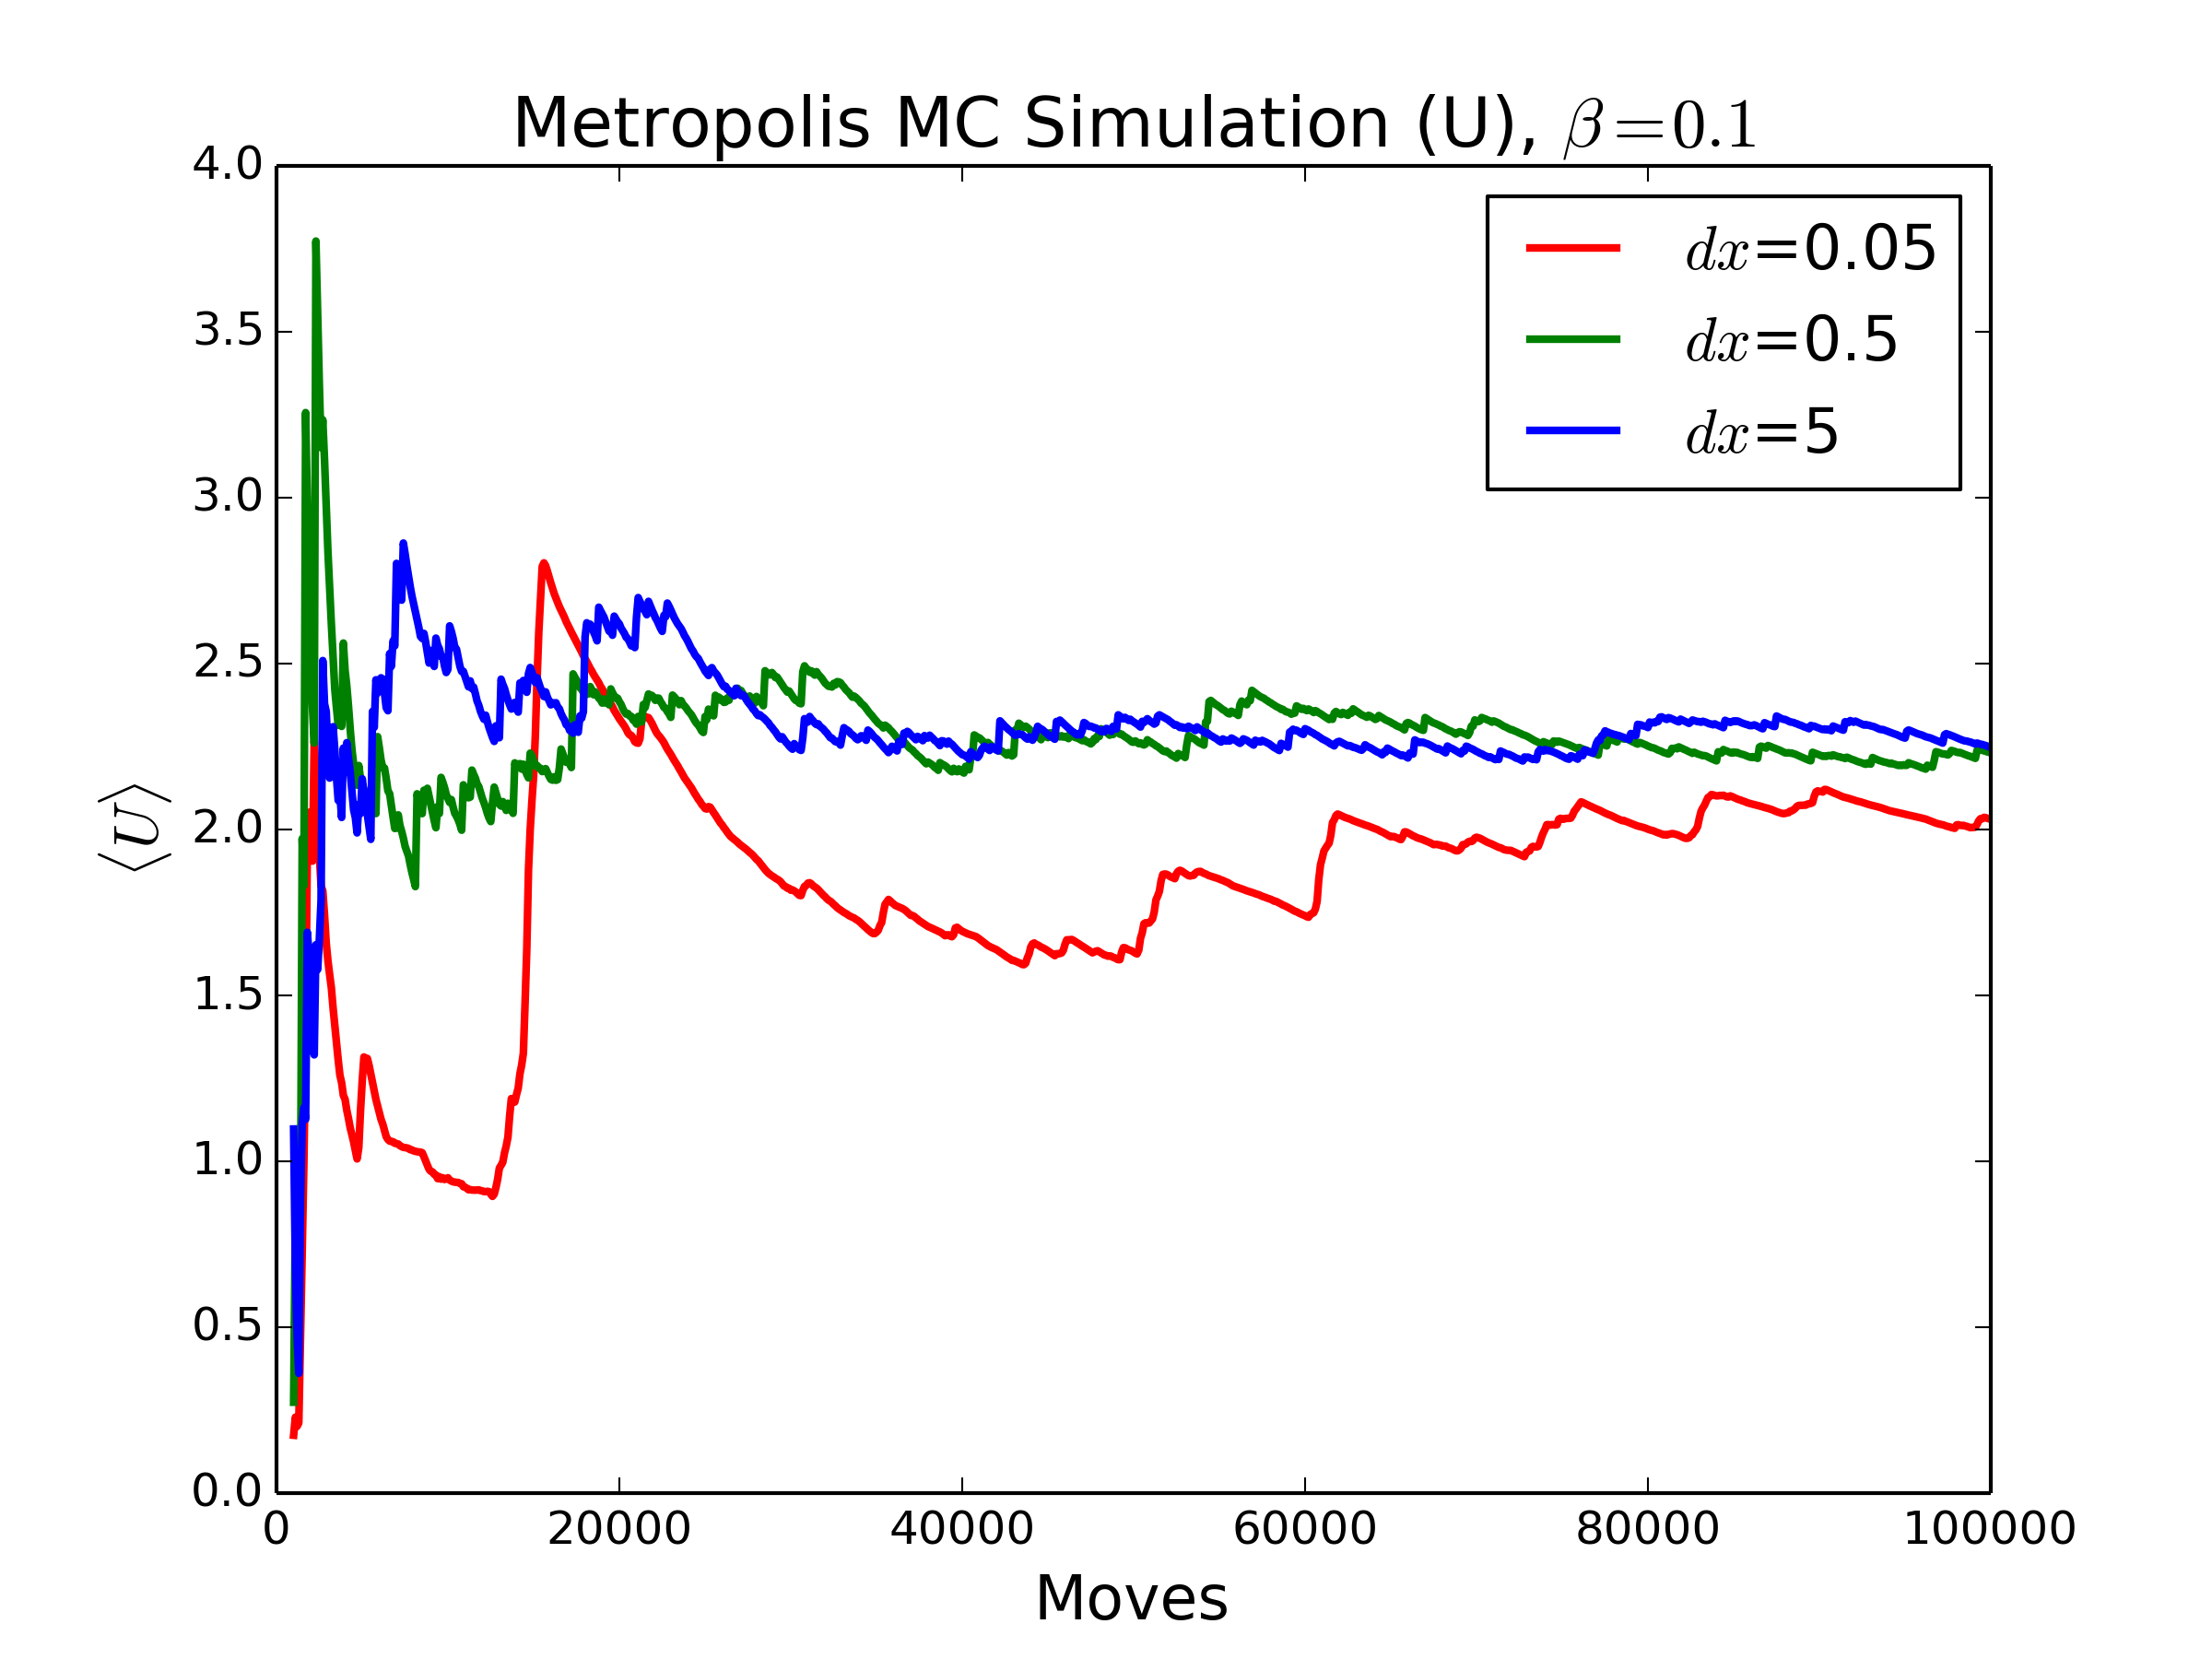
\includegraphics[width=0.49\textwidth]{./P2/part-b-beta-0.1/Oscillator2a-U.png}\label{fig:f1}}
  \hfill
\subfloat{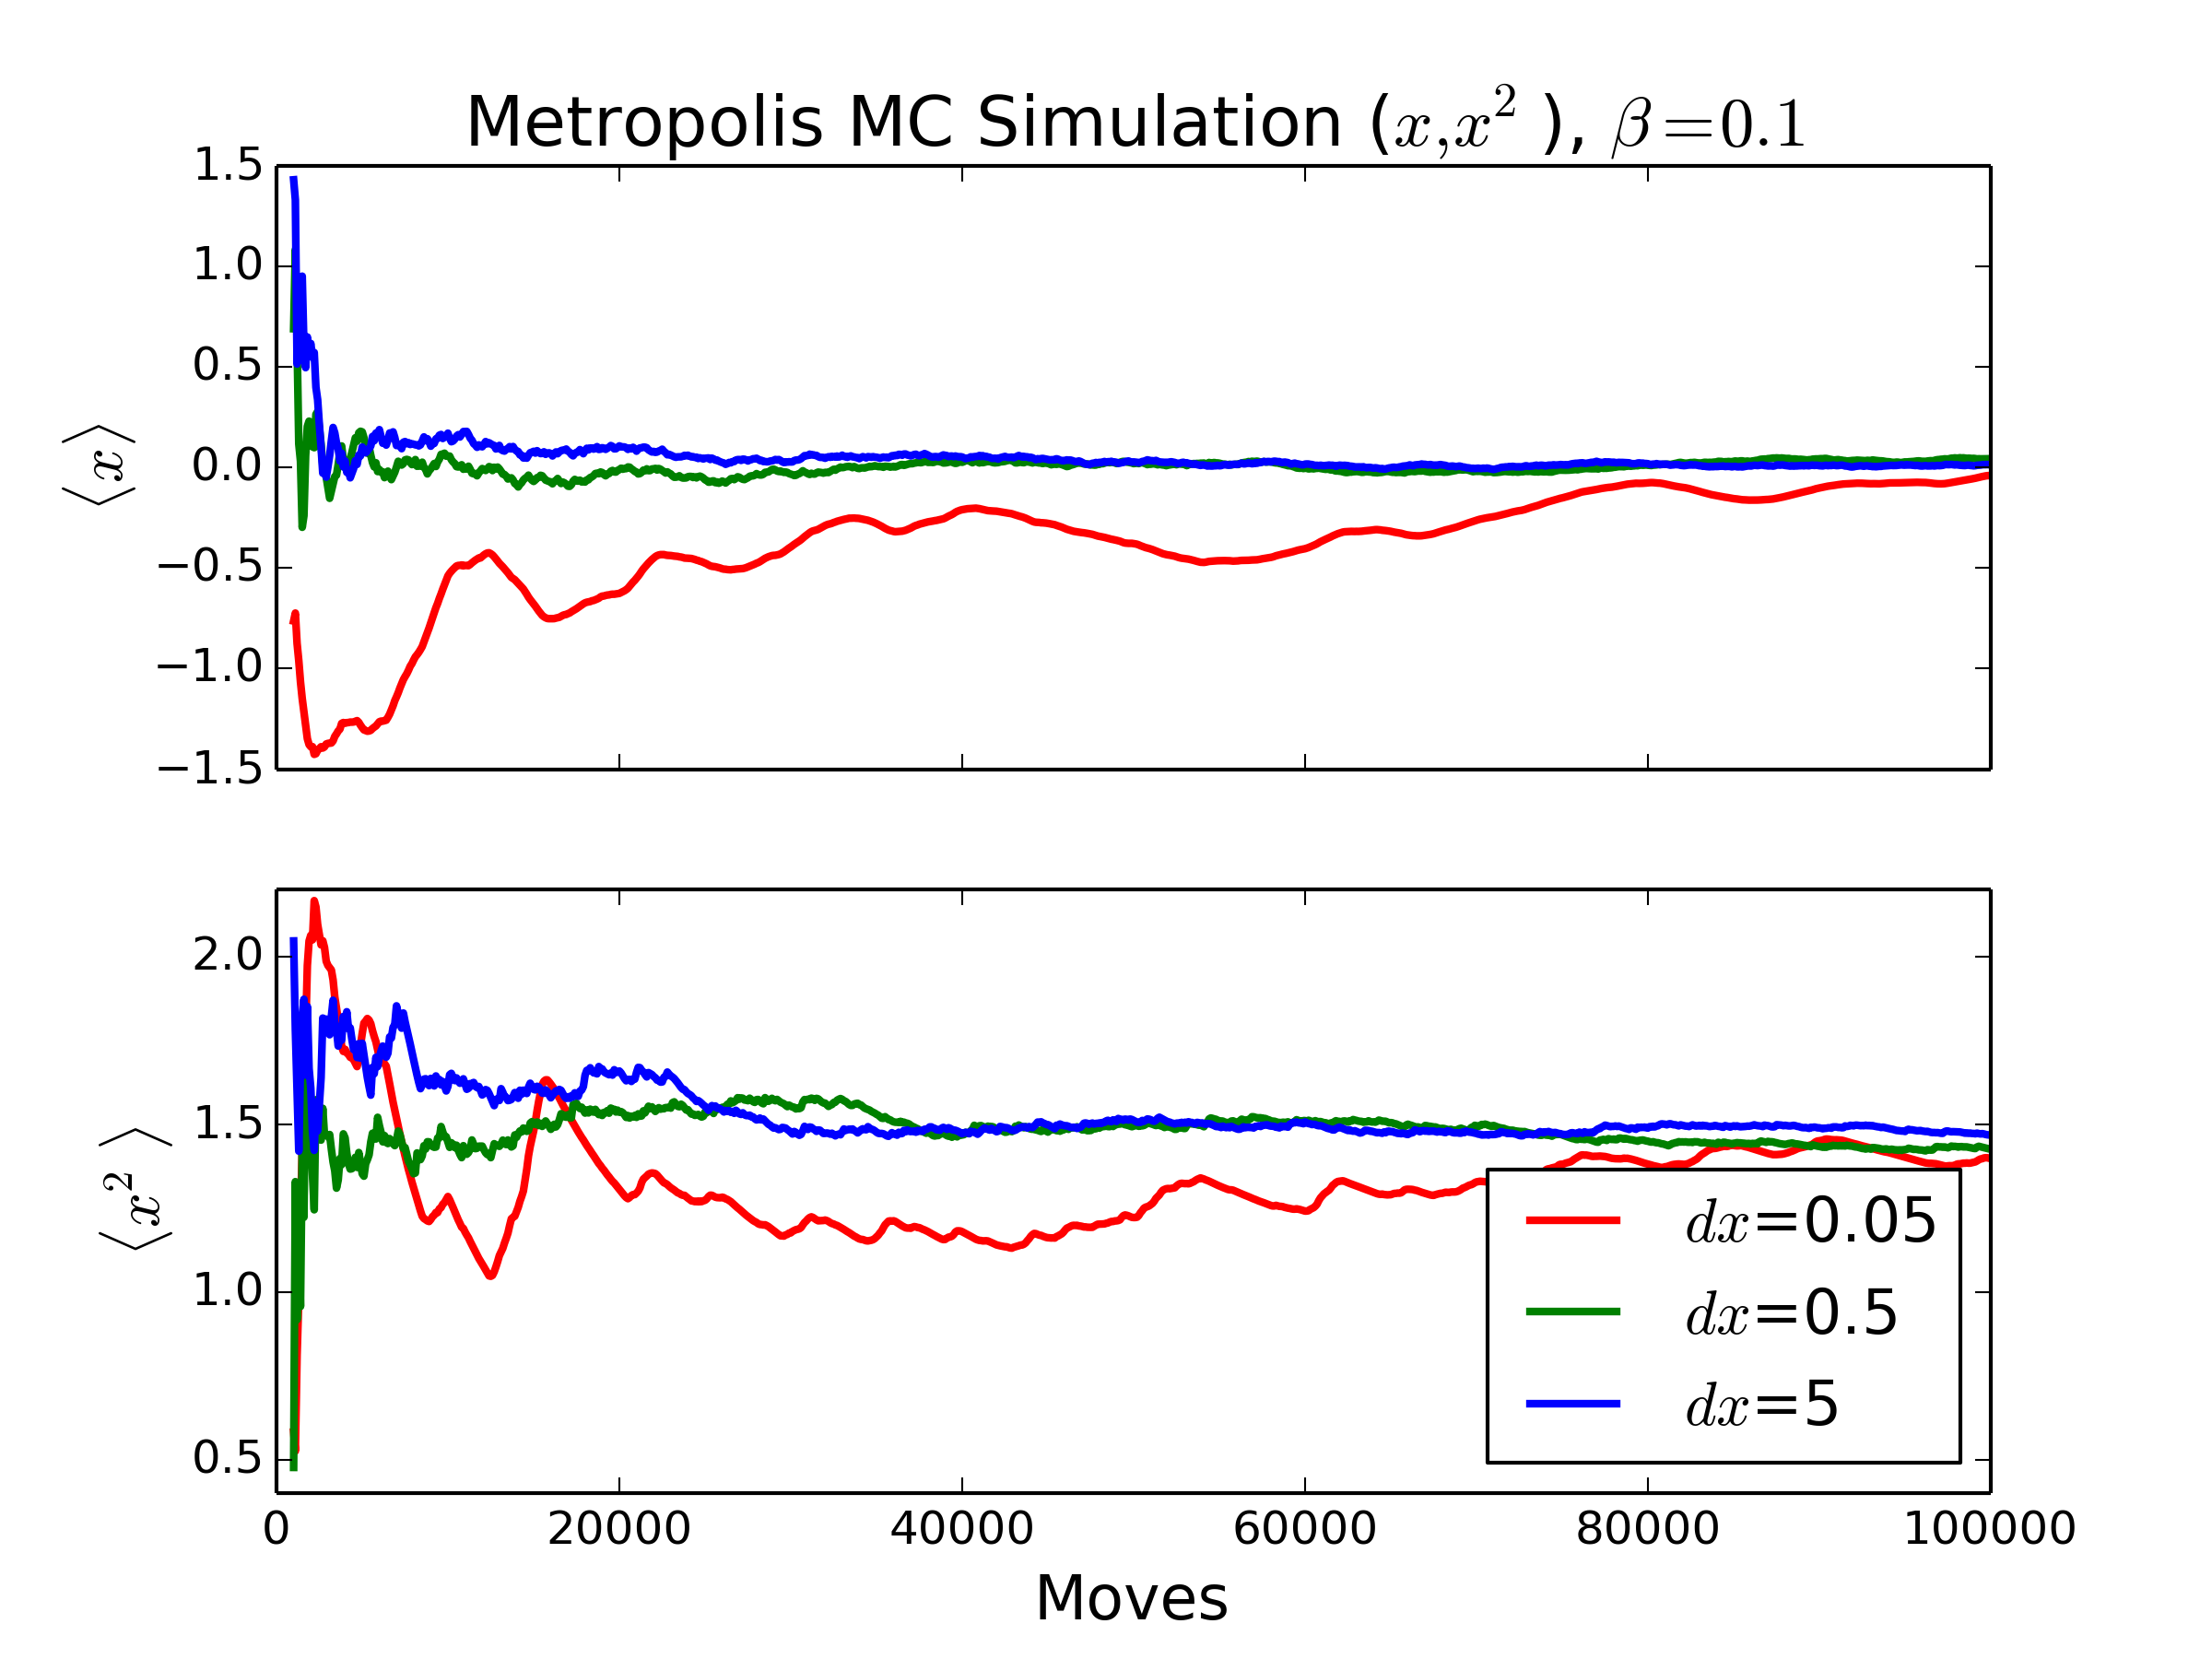
\includegraphics[width=0.49\textwidth]{./P2/part-b-beta-0.1/Oscillator2a-x.png}\label{fig:f1}}
  \caption{Monte Carlo Simulation of oscillator at \beta=0.1}
  \label{fig:1b-01}
\end{figure}

\begin{figure}[!tbp]
  \centering
\subfloat{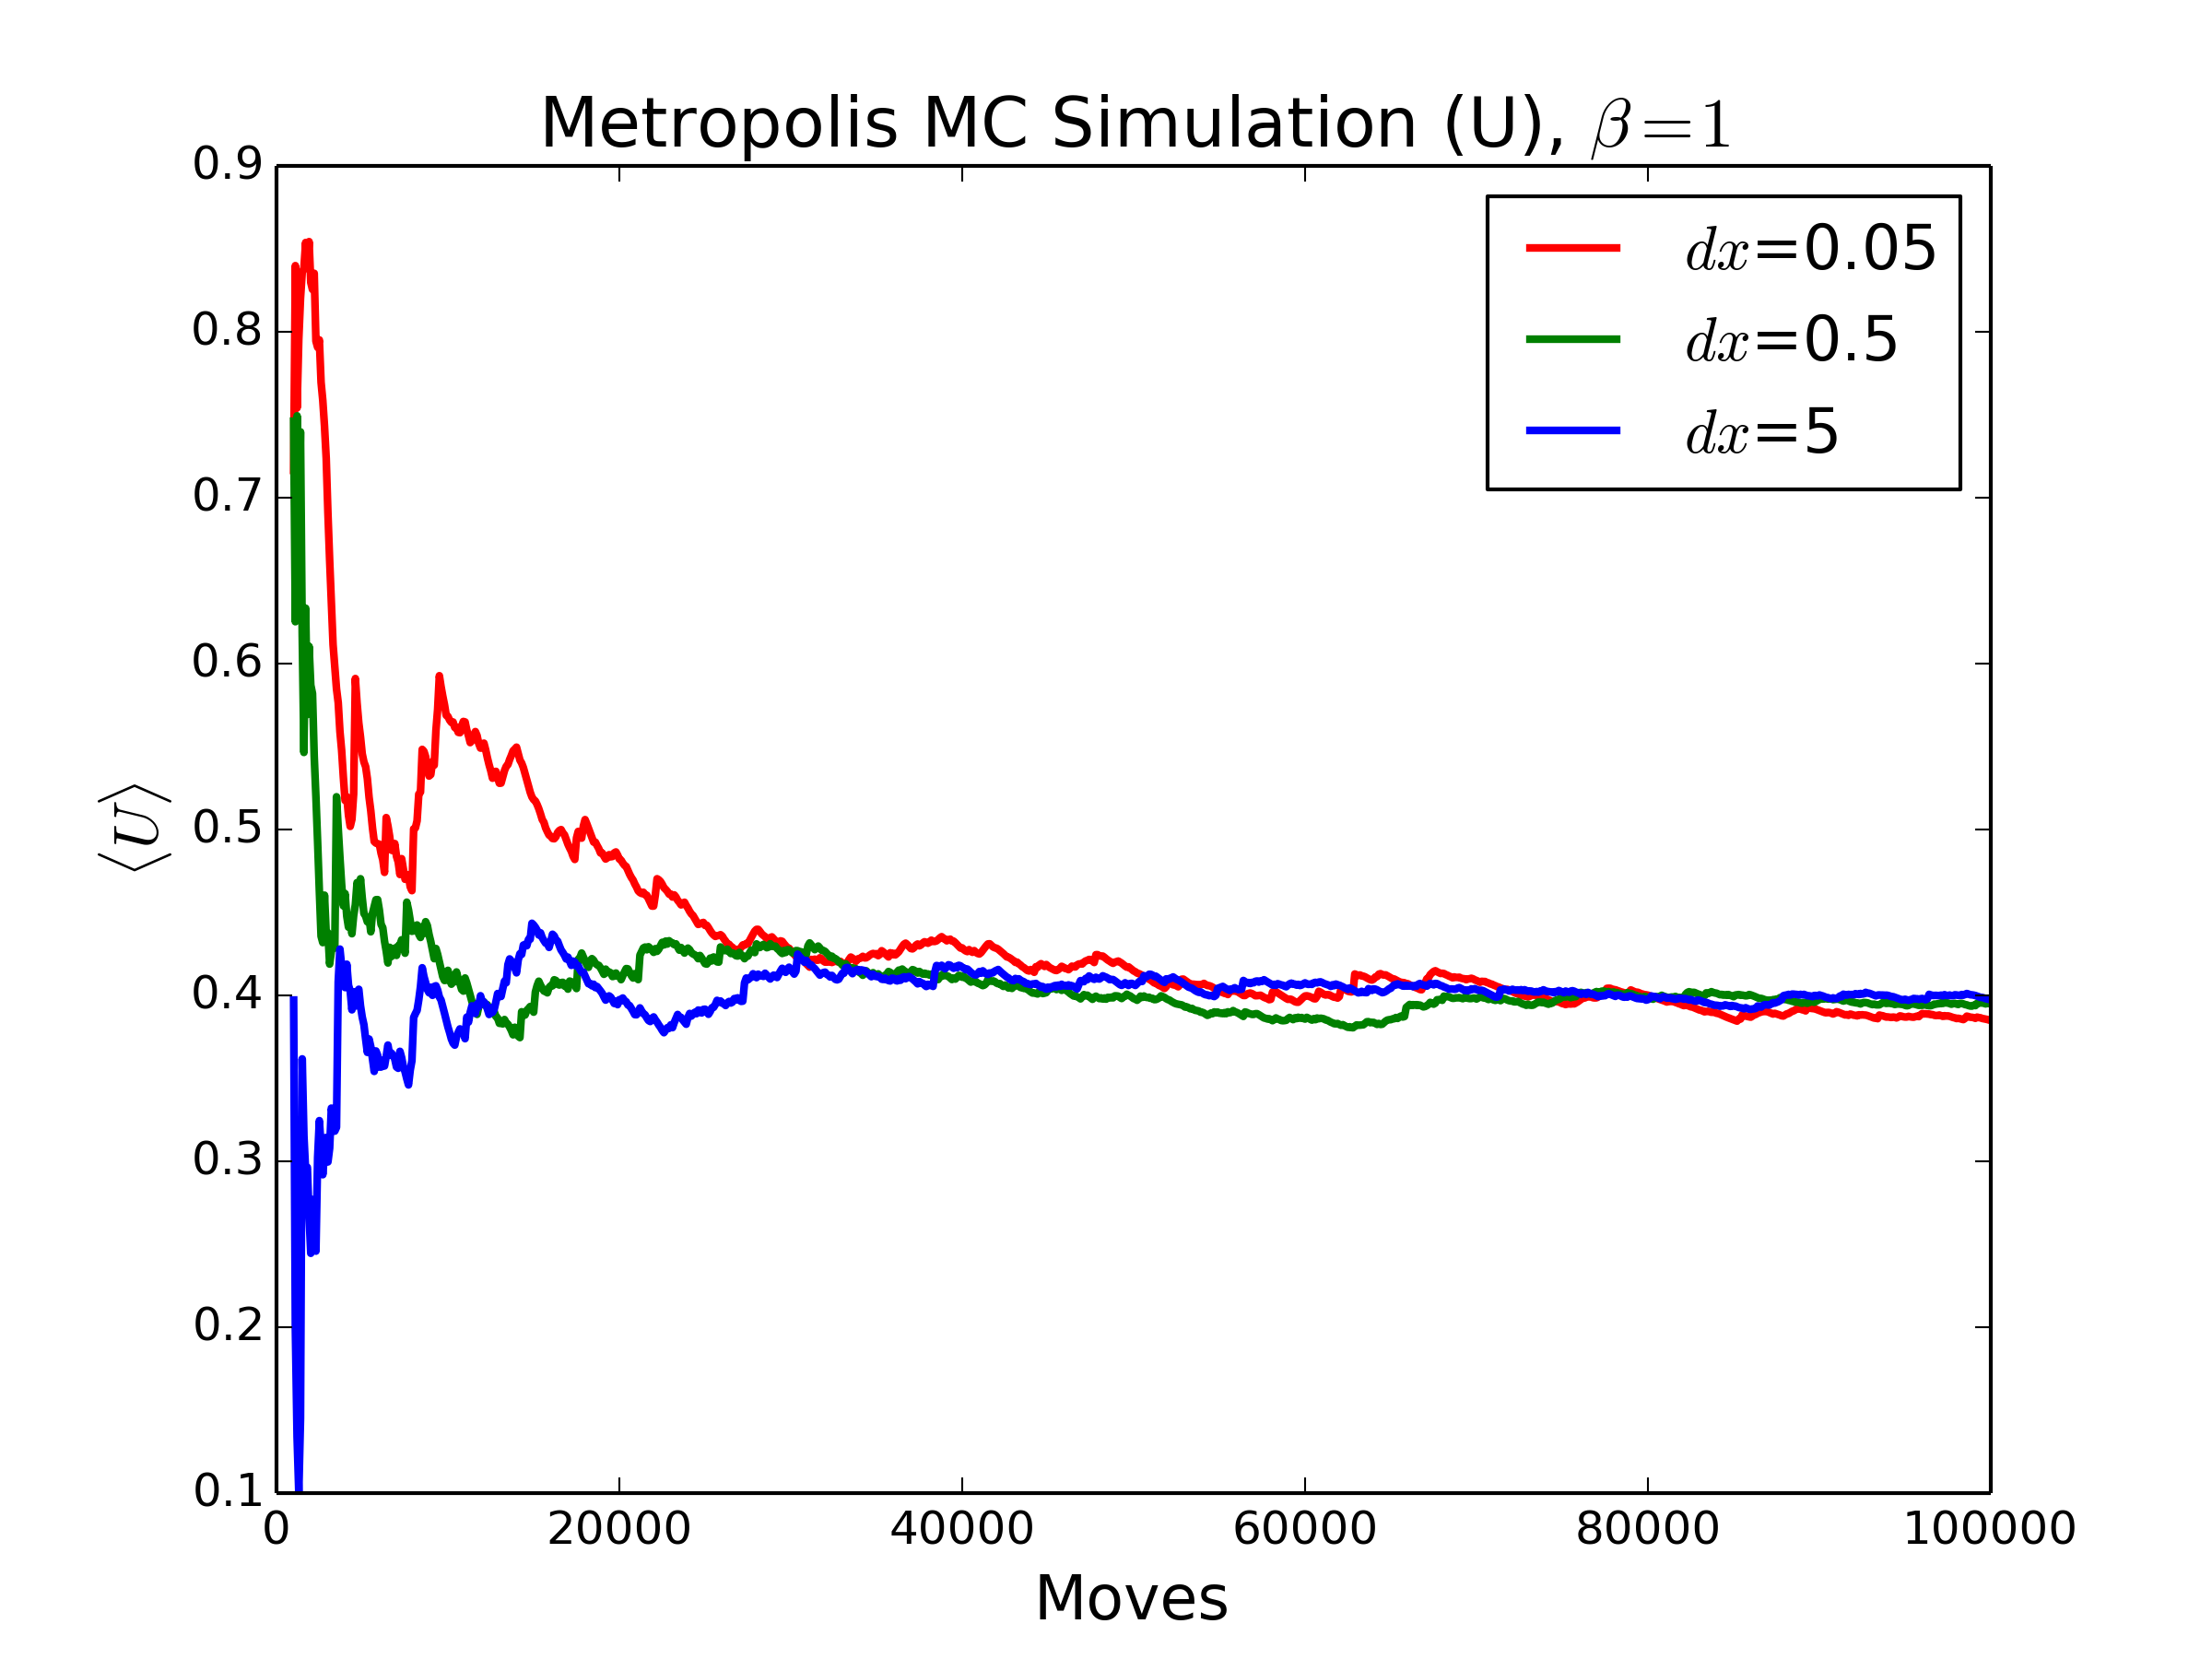
\includegraphics[width=0.49\textwidth]{./P2/part-b-beta-1/Oscillator2a-U.png}\label{fig:f1}}
  \hfill
\subfloat{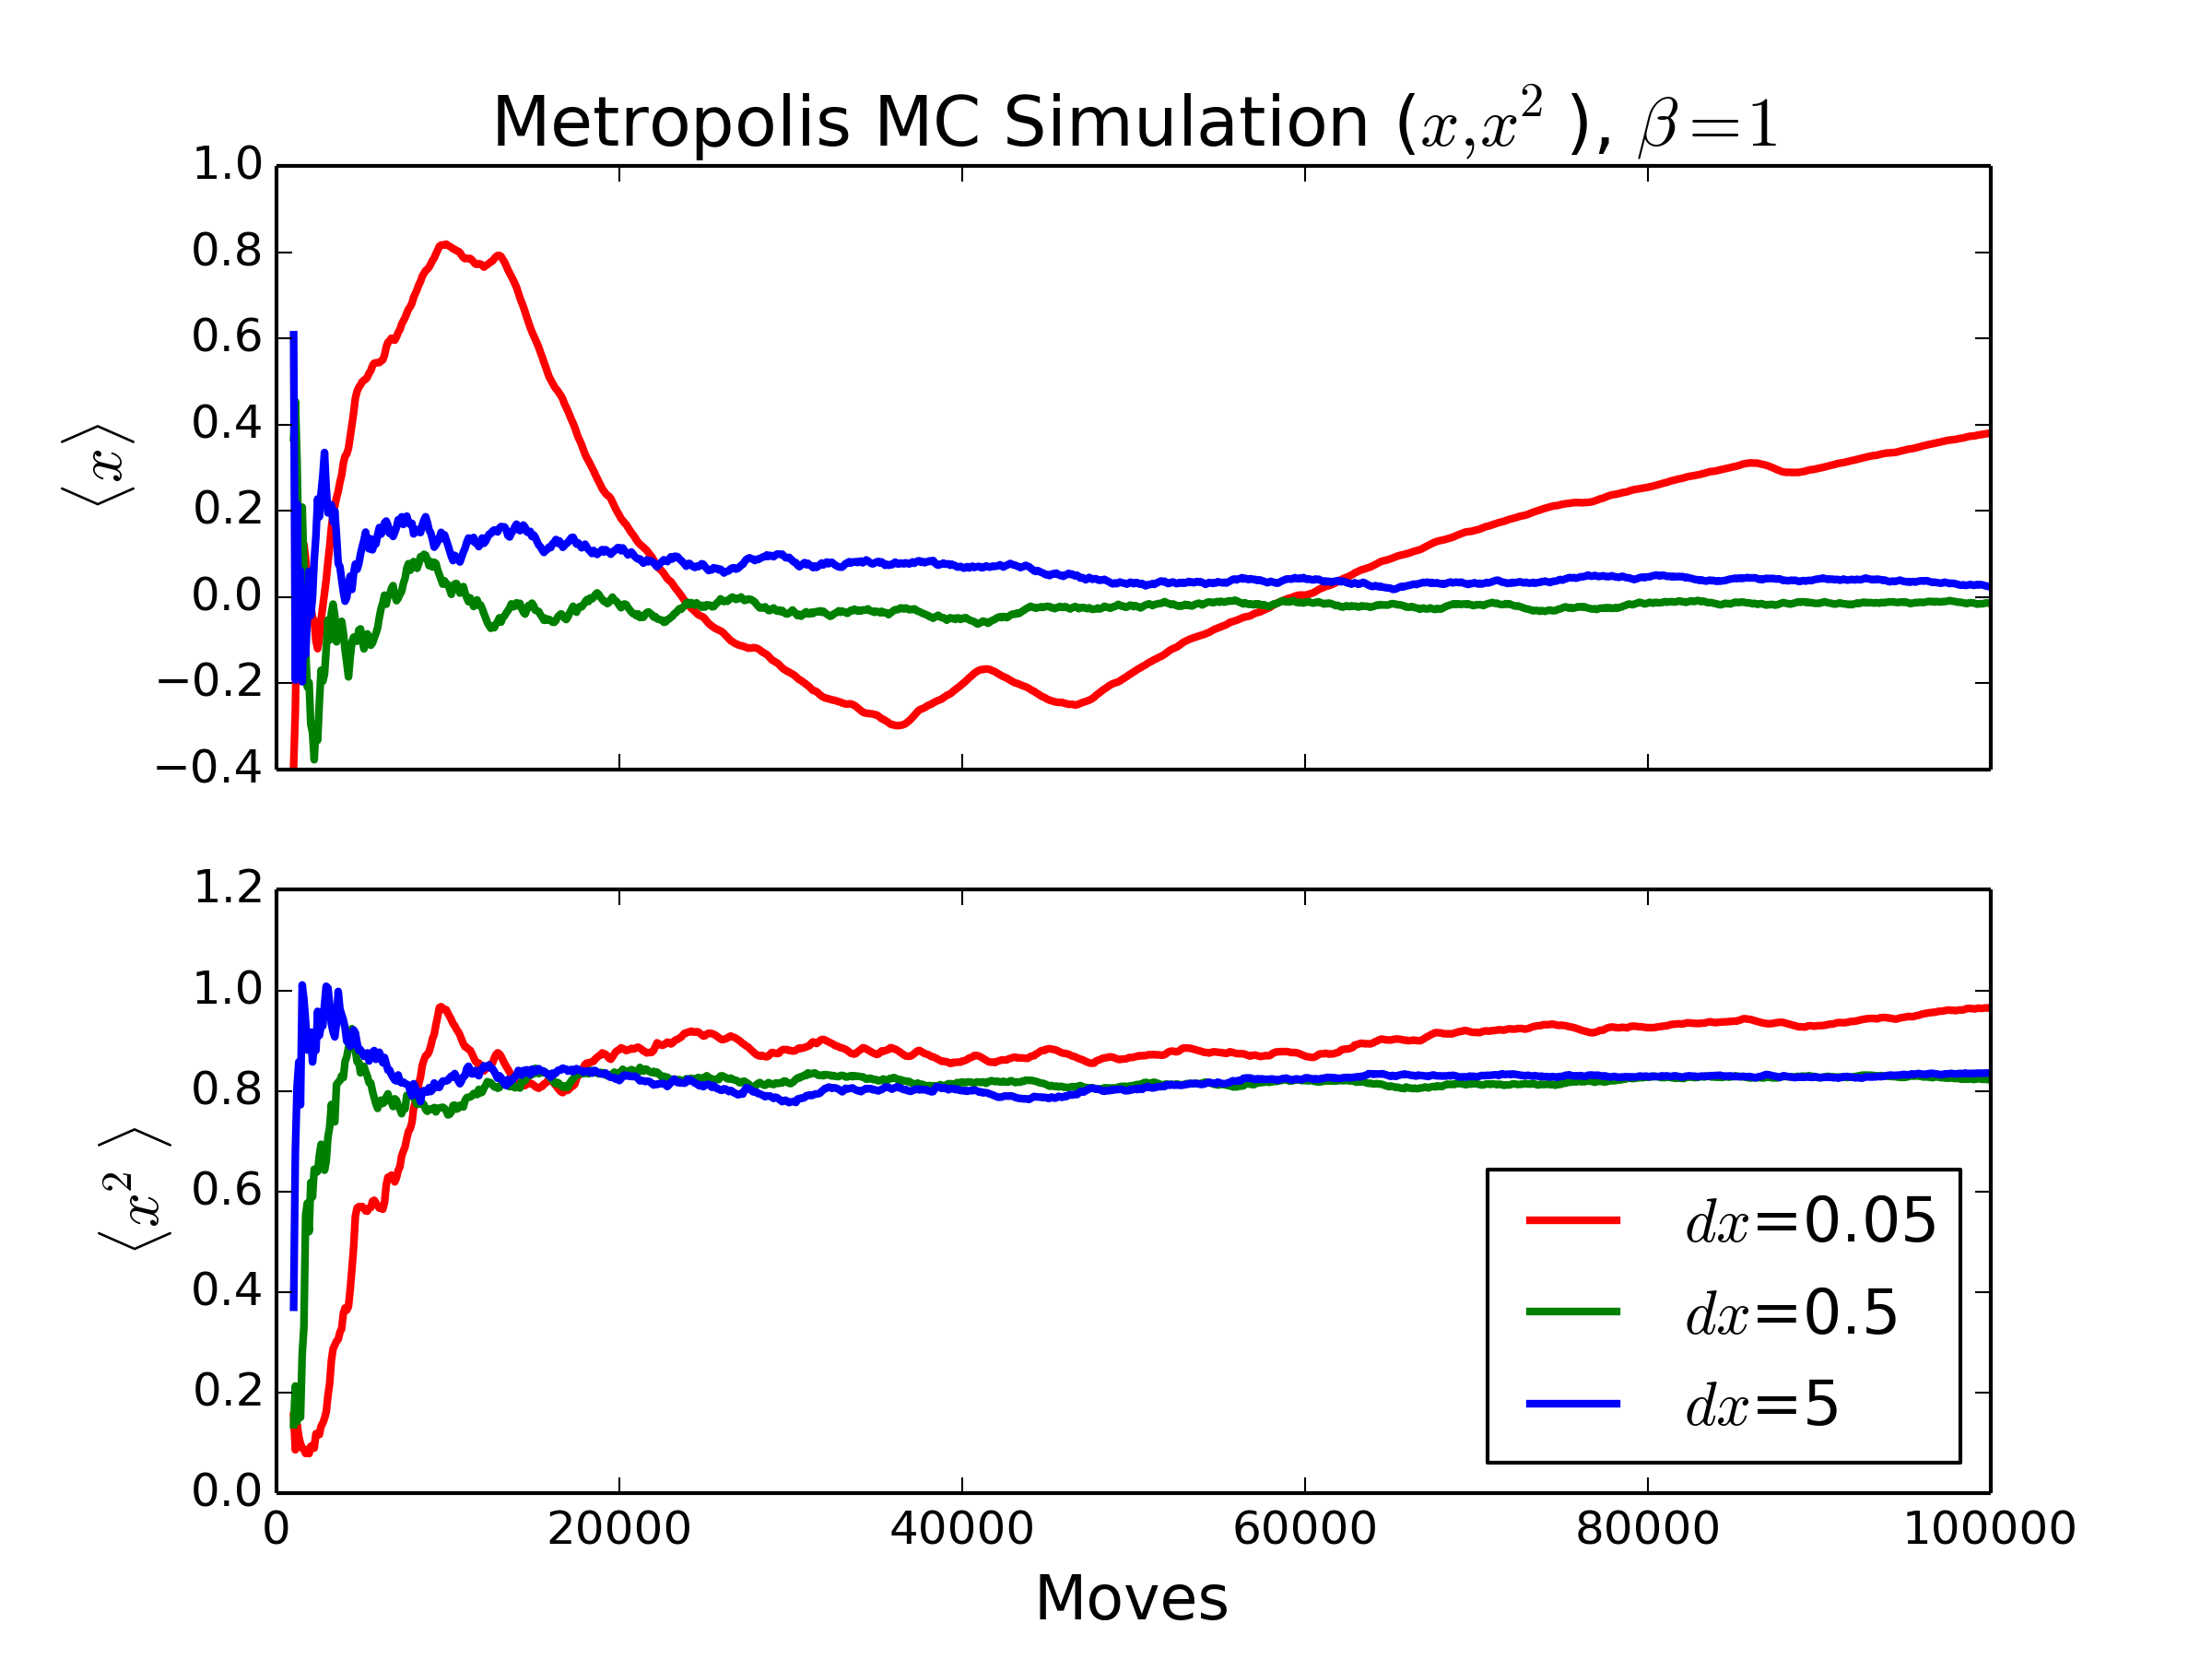
\includegraphics[width=0.49\textwidth]{./P2/part-b-beta-1/Oscillator2a-x.png}\label{fig:f1}}
  \caption{Monte Carlo Simulation of oscillator at \beta=1}
  \label{fig:1b-1}
\end{figure}

\begin{figure}[!tbp]
  \centering
\subfloat{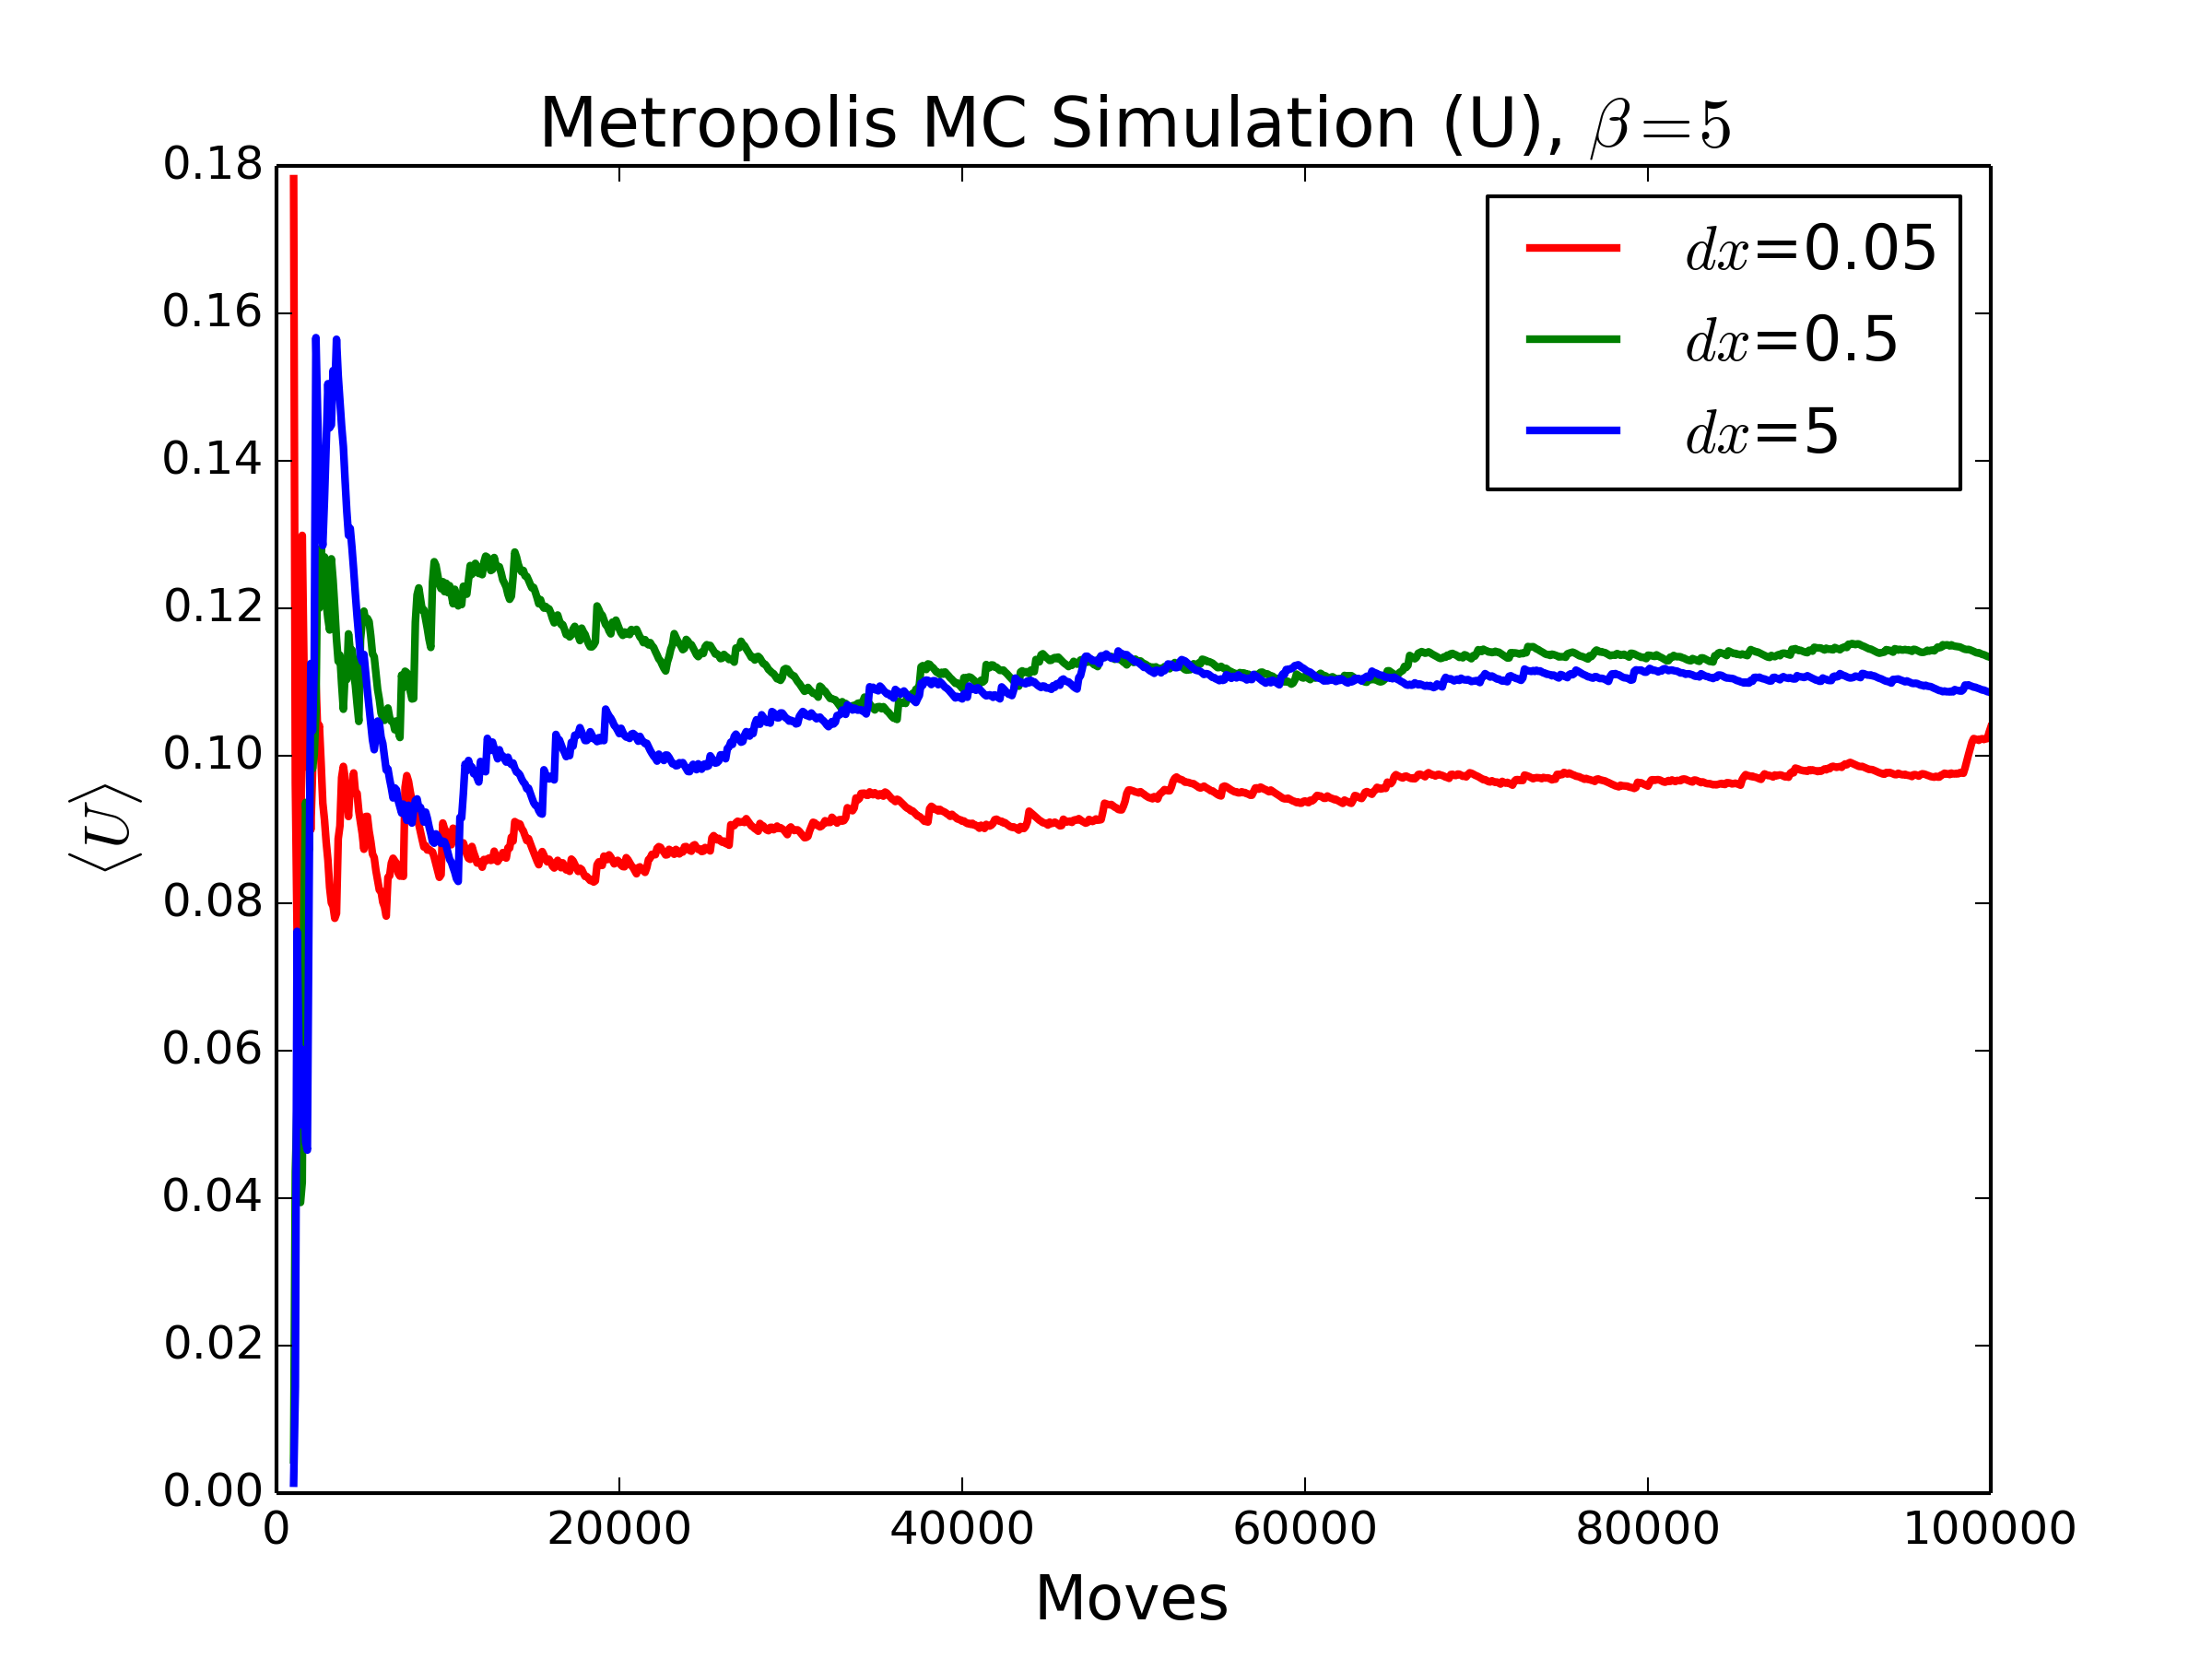
\includegraphics[width=0.49\textwidth]{./P2/part-b-beta-5/Oscillator2a-U.png}\label{fig:f1}}
  \hfill
\subfloat{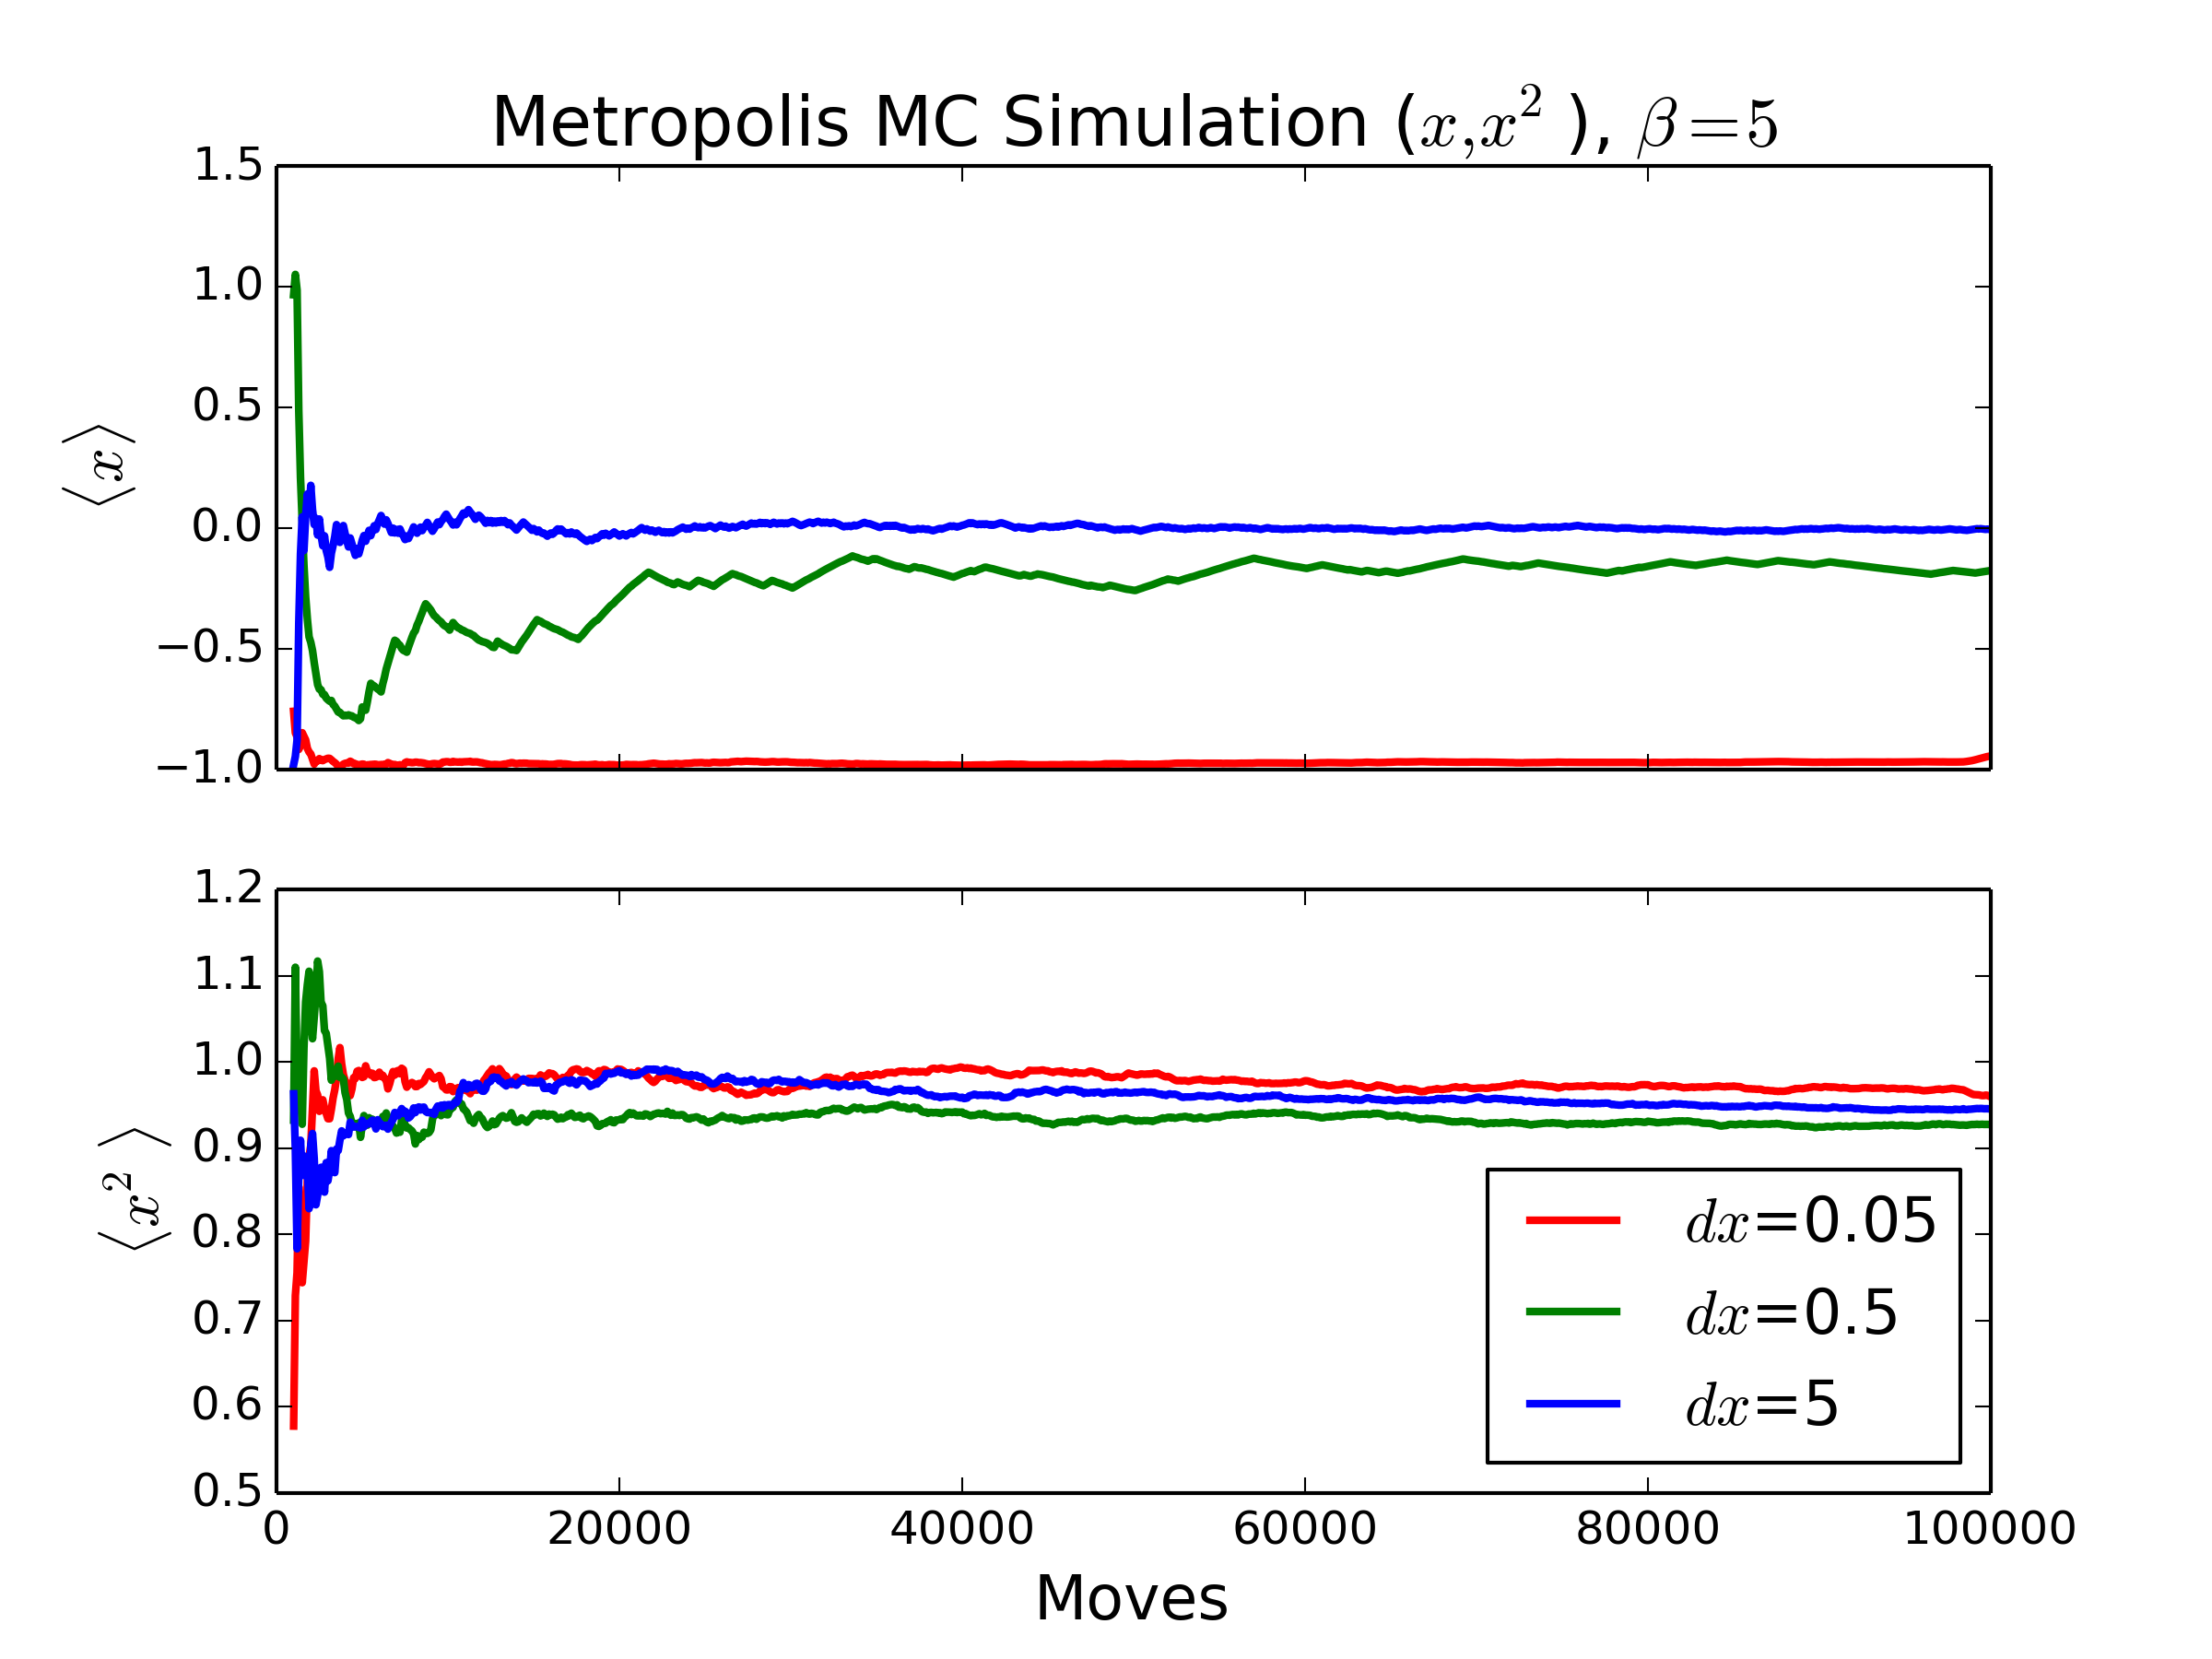
\includegraphics[width=0.49\textwidth]{./P2/part-b-beta-5/Oscillator2a-x.png}\label{fig:f1}}
  \caption{Monte Carlo Simulation of oscillator at \beta=5}
  \label{fig:1b-5}
\end{figure}

\begin{figure}[!tbp]
  \centering
\subfloat{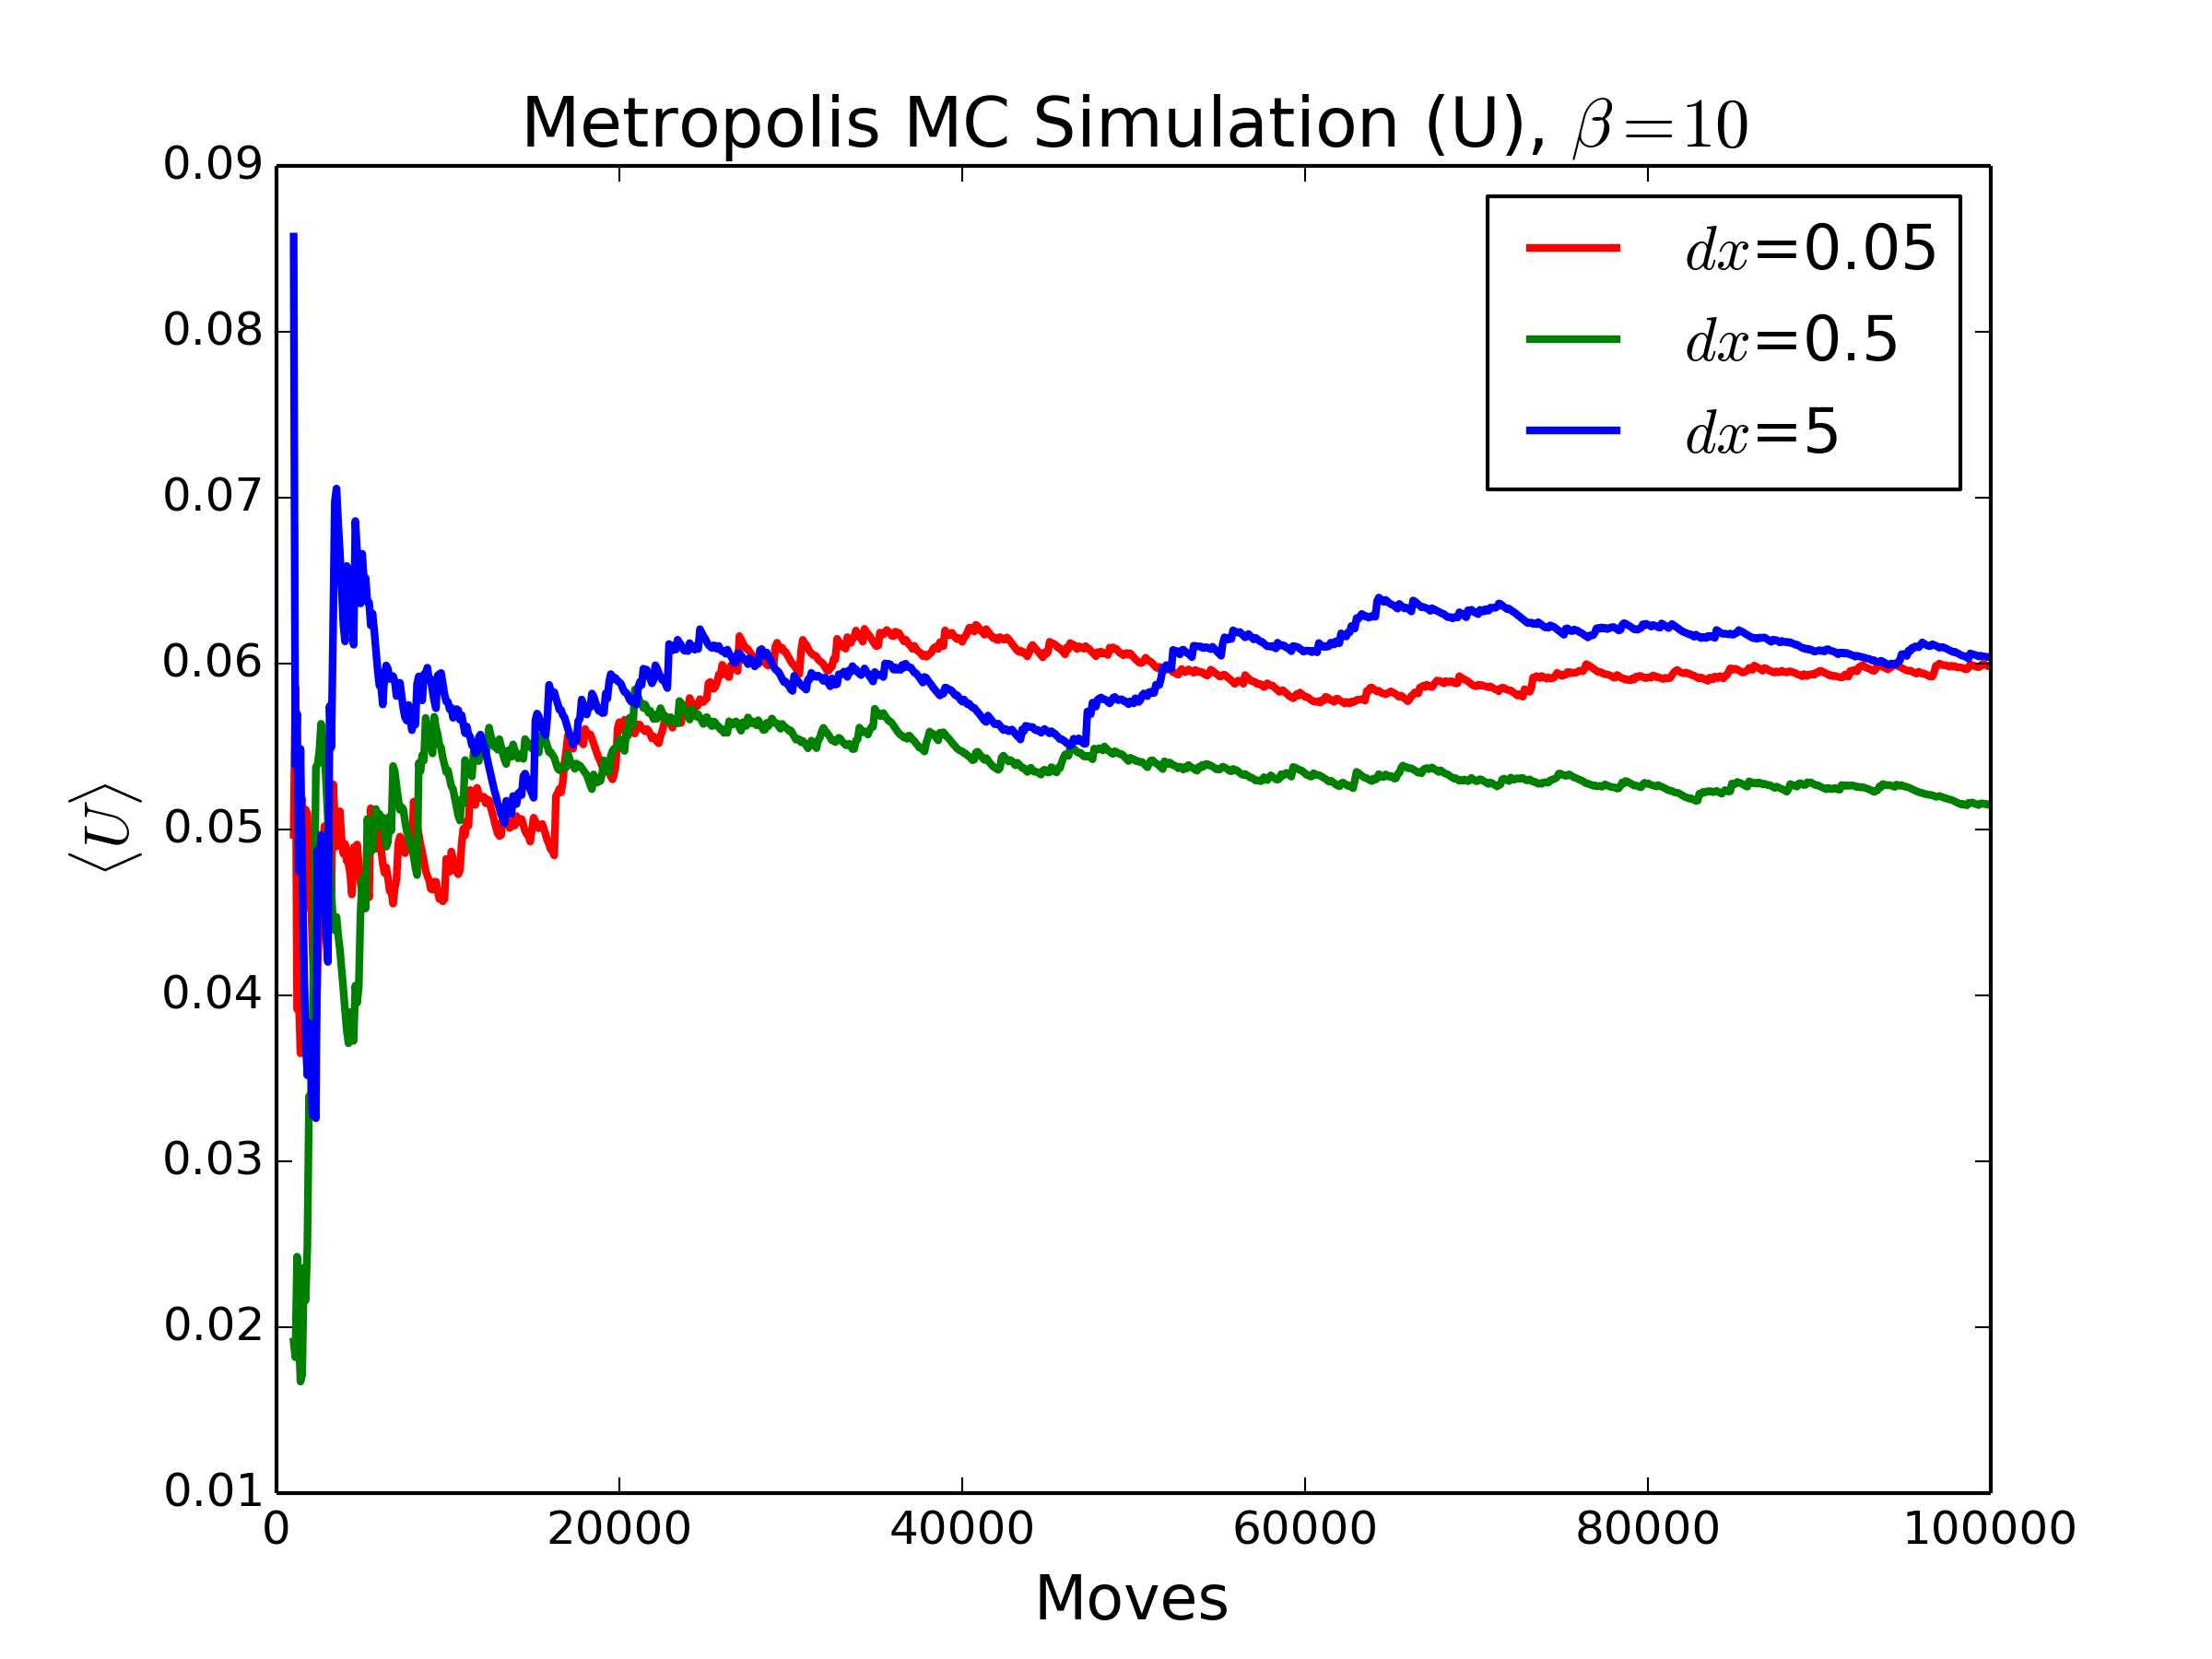
\includegraphics[width=0.49\textwidth]{./P2/part-b-beta-10/Oscillator2a-U.png}\label{fig:f1}}
  \hfill
\subfloat{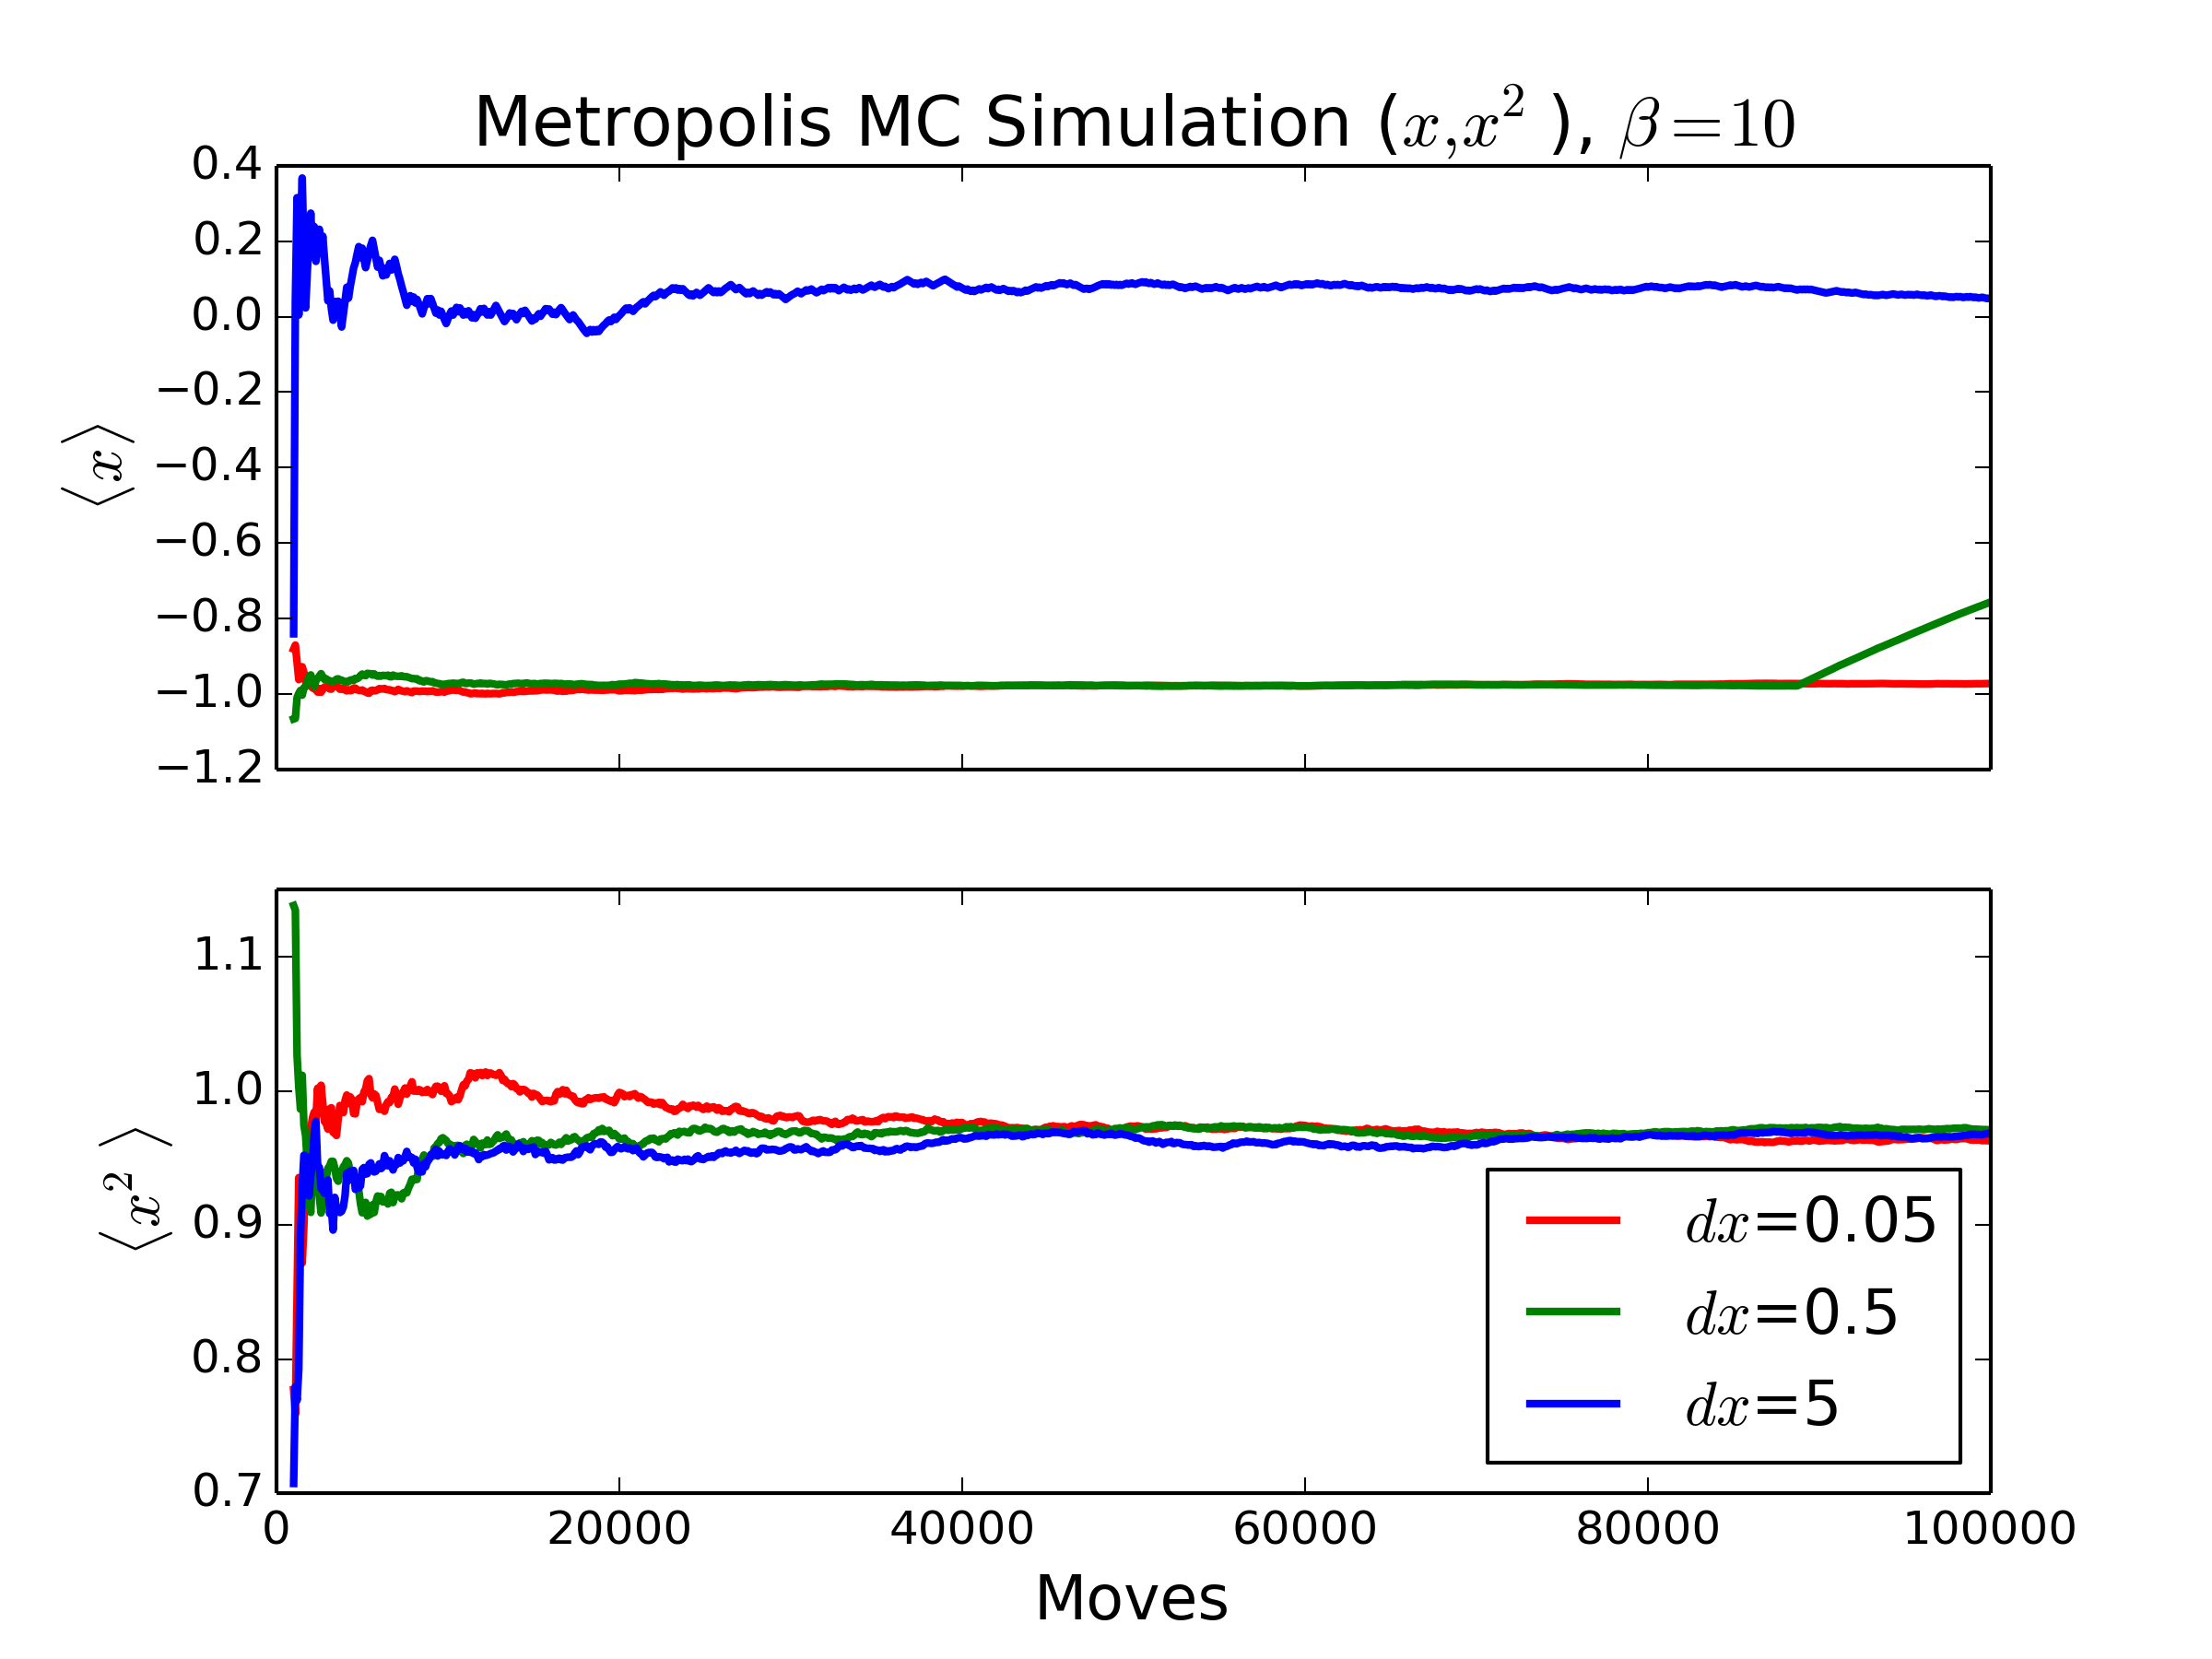
\includegraphics[width=0.49\textwidth]{./P2/part-b-beta-10/Oscillator2a-x.png}\label{fig:f1}}
  \caption{Monte Carlo Simulation of oscillator at \beta=10}
  \label{fig:1b-10}
\end{figure}

\section{Bonus}
\label{sec-3}

Monte Carlo computations are performed with Kawasaki dynamics and an interesting feature is observed for the percentage of accepted moves. It is observed that the accpetance percentage of the moves increases when compared to the metropolis monte carlo.

\begin{table}[htb]
\caption{\label{tab:table2}Percentage of acceptance of the moves with respect to various values of $\beta$ and  max. step sizes is shown below.}
\centering
\begin{tabular}{rrrrr}
\hline
$\delta$ dx$_{\text{max}}$ & $\beta$=0.1 & $\beta$=1 & $\beta$=5 & $\beta$=10\\
\hline
0.05 & 50.231 & 50.205 & 49.819 & 50.168\\
0.5 & 50.194 & 48.93 & 45.499 & 42.05\\
5 & 42.103 & 20.209 & 9.138 & 6.509\\
\hline
\end{tabular}
\end{table}

\begin{figure}[!tbp]
  \centering
\subfloat{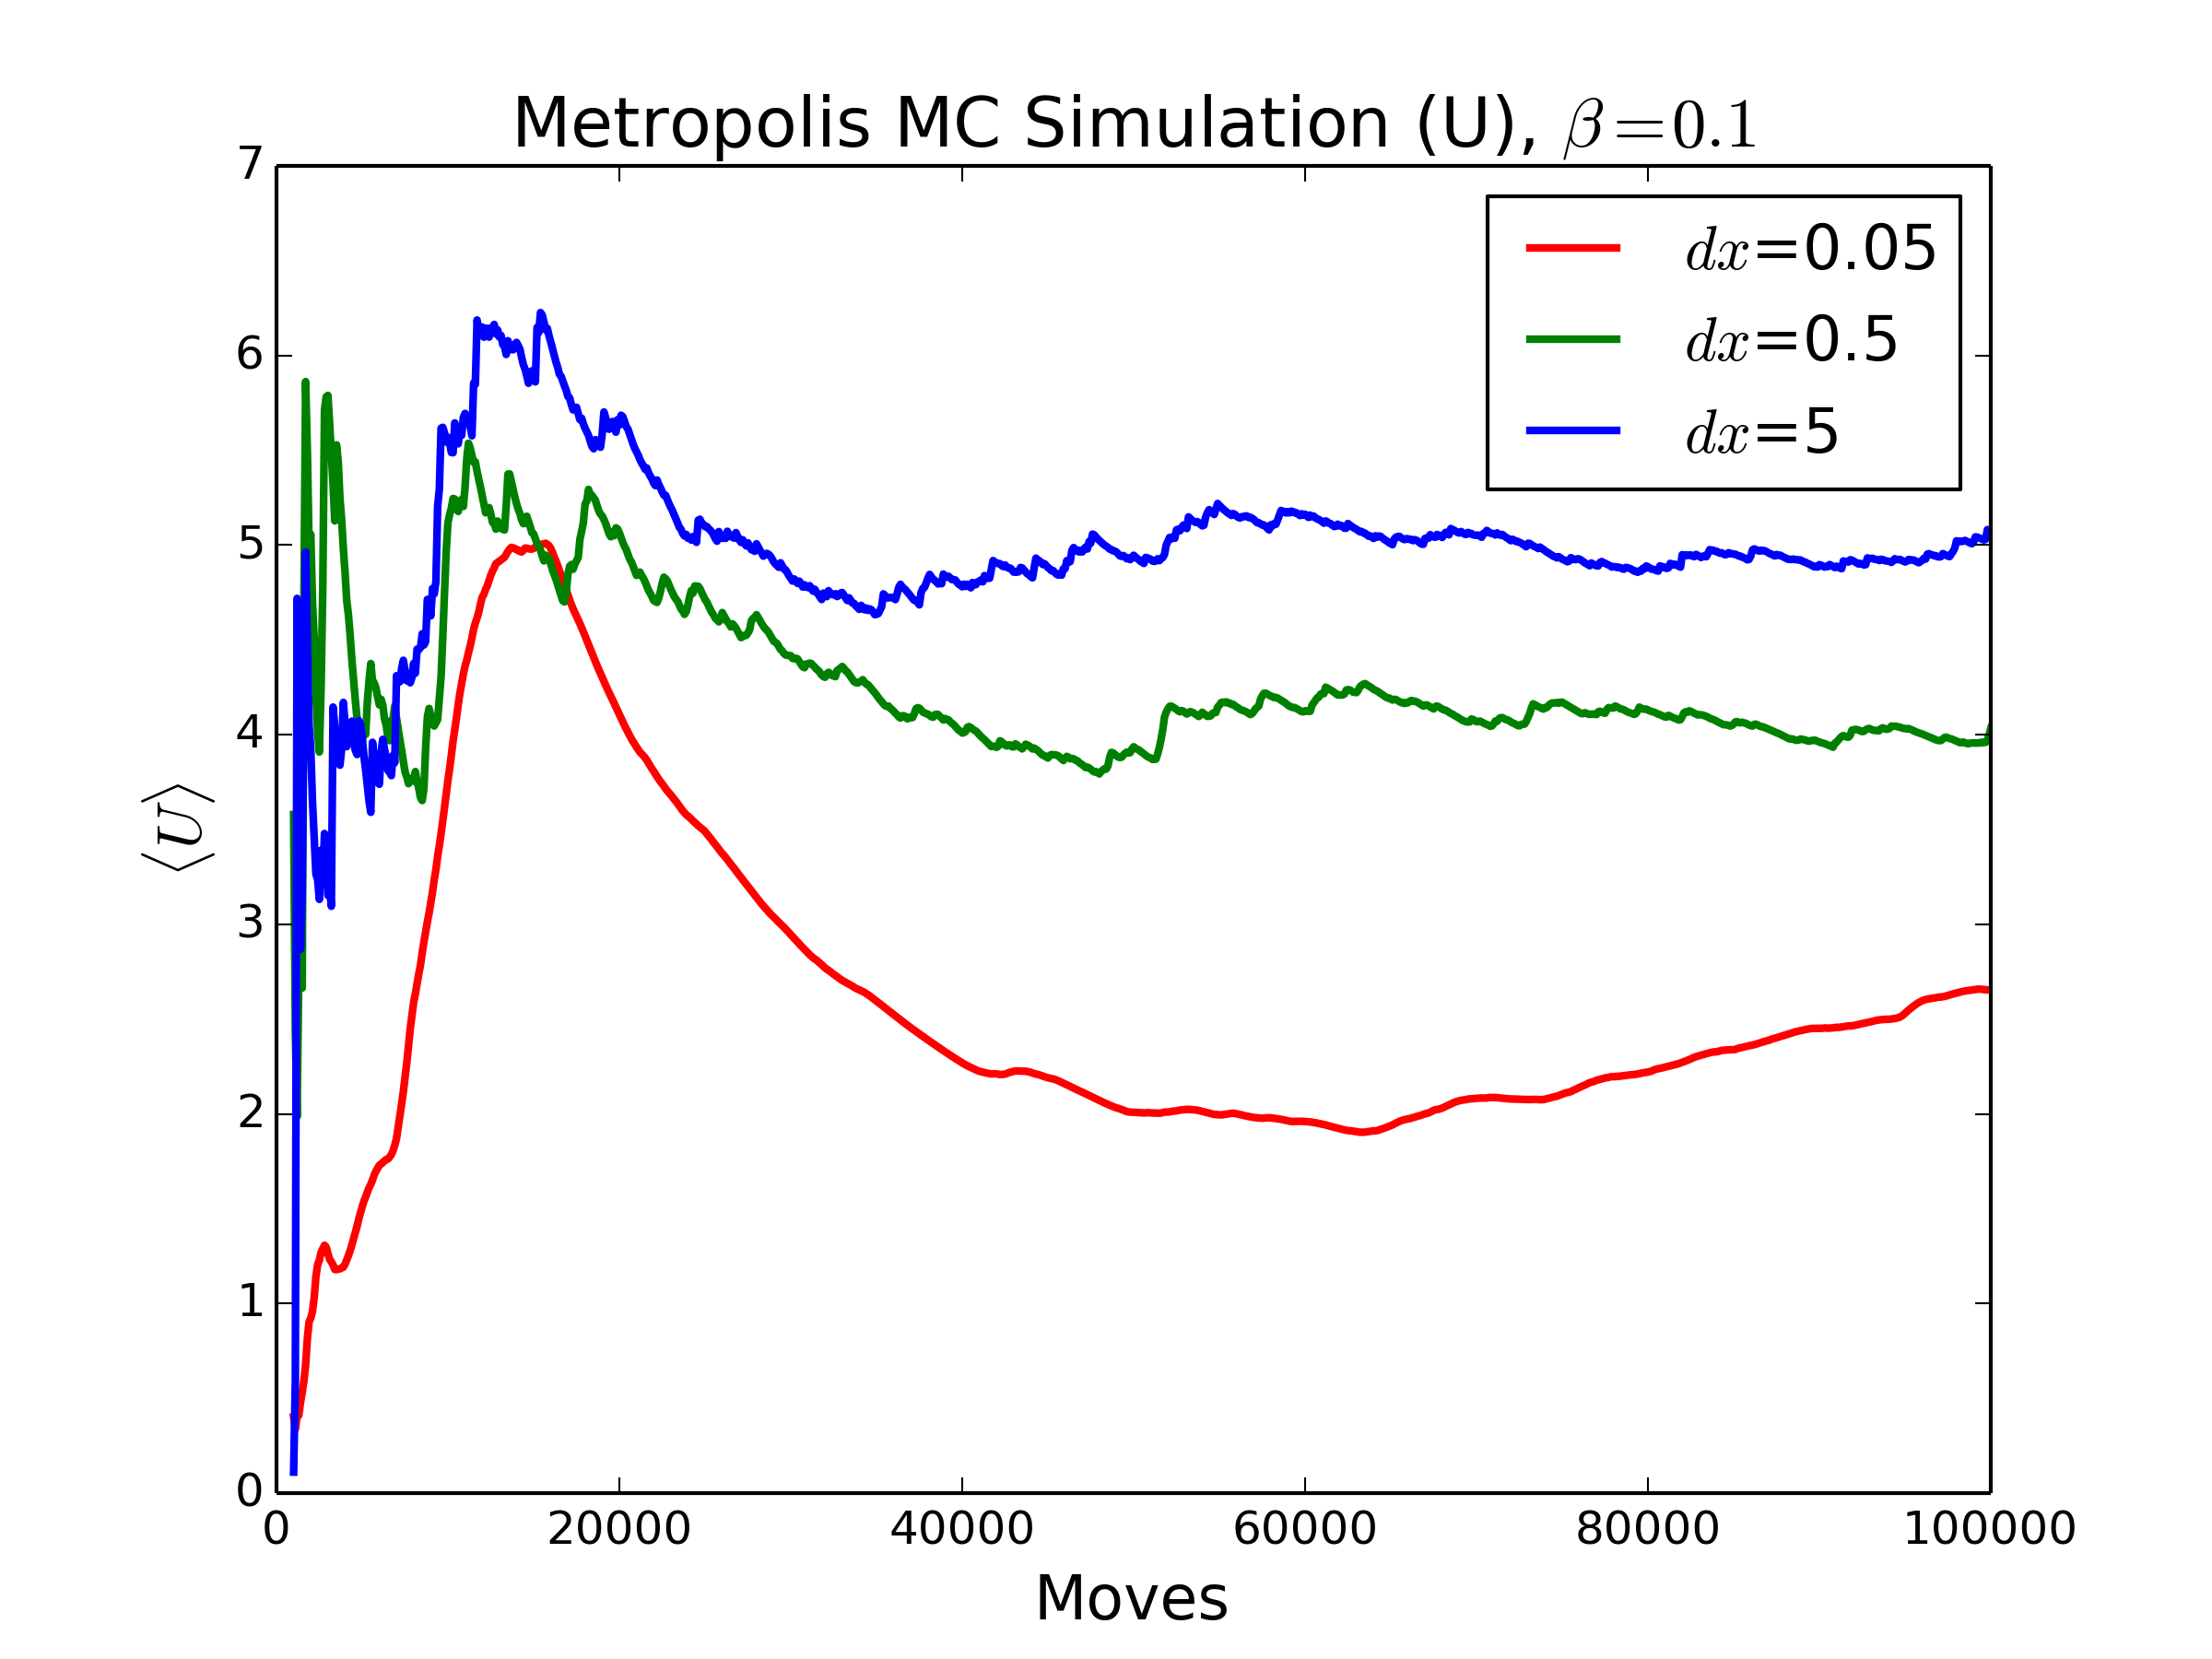
\includegraphics[width=0.49\textwidth]{./bonus/part-a-beta-0.1/Oscillator2a-U.png}\label{fig:f1}}
  \hfill
\subfloat{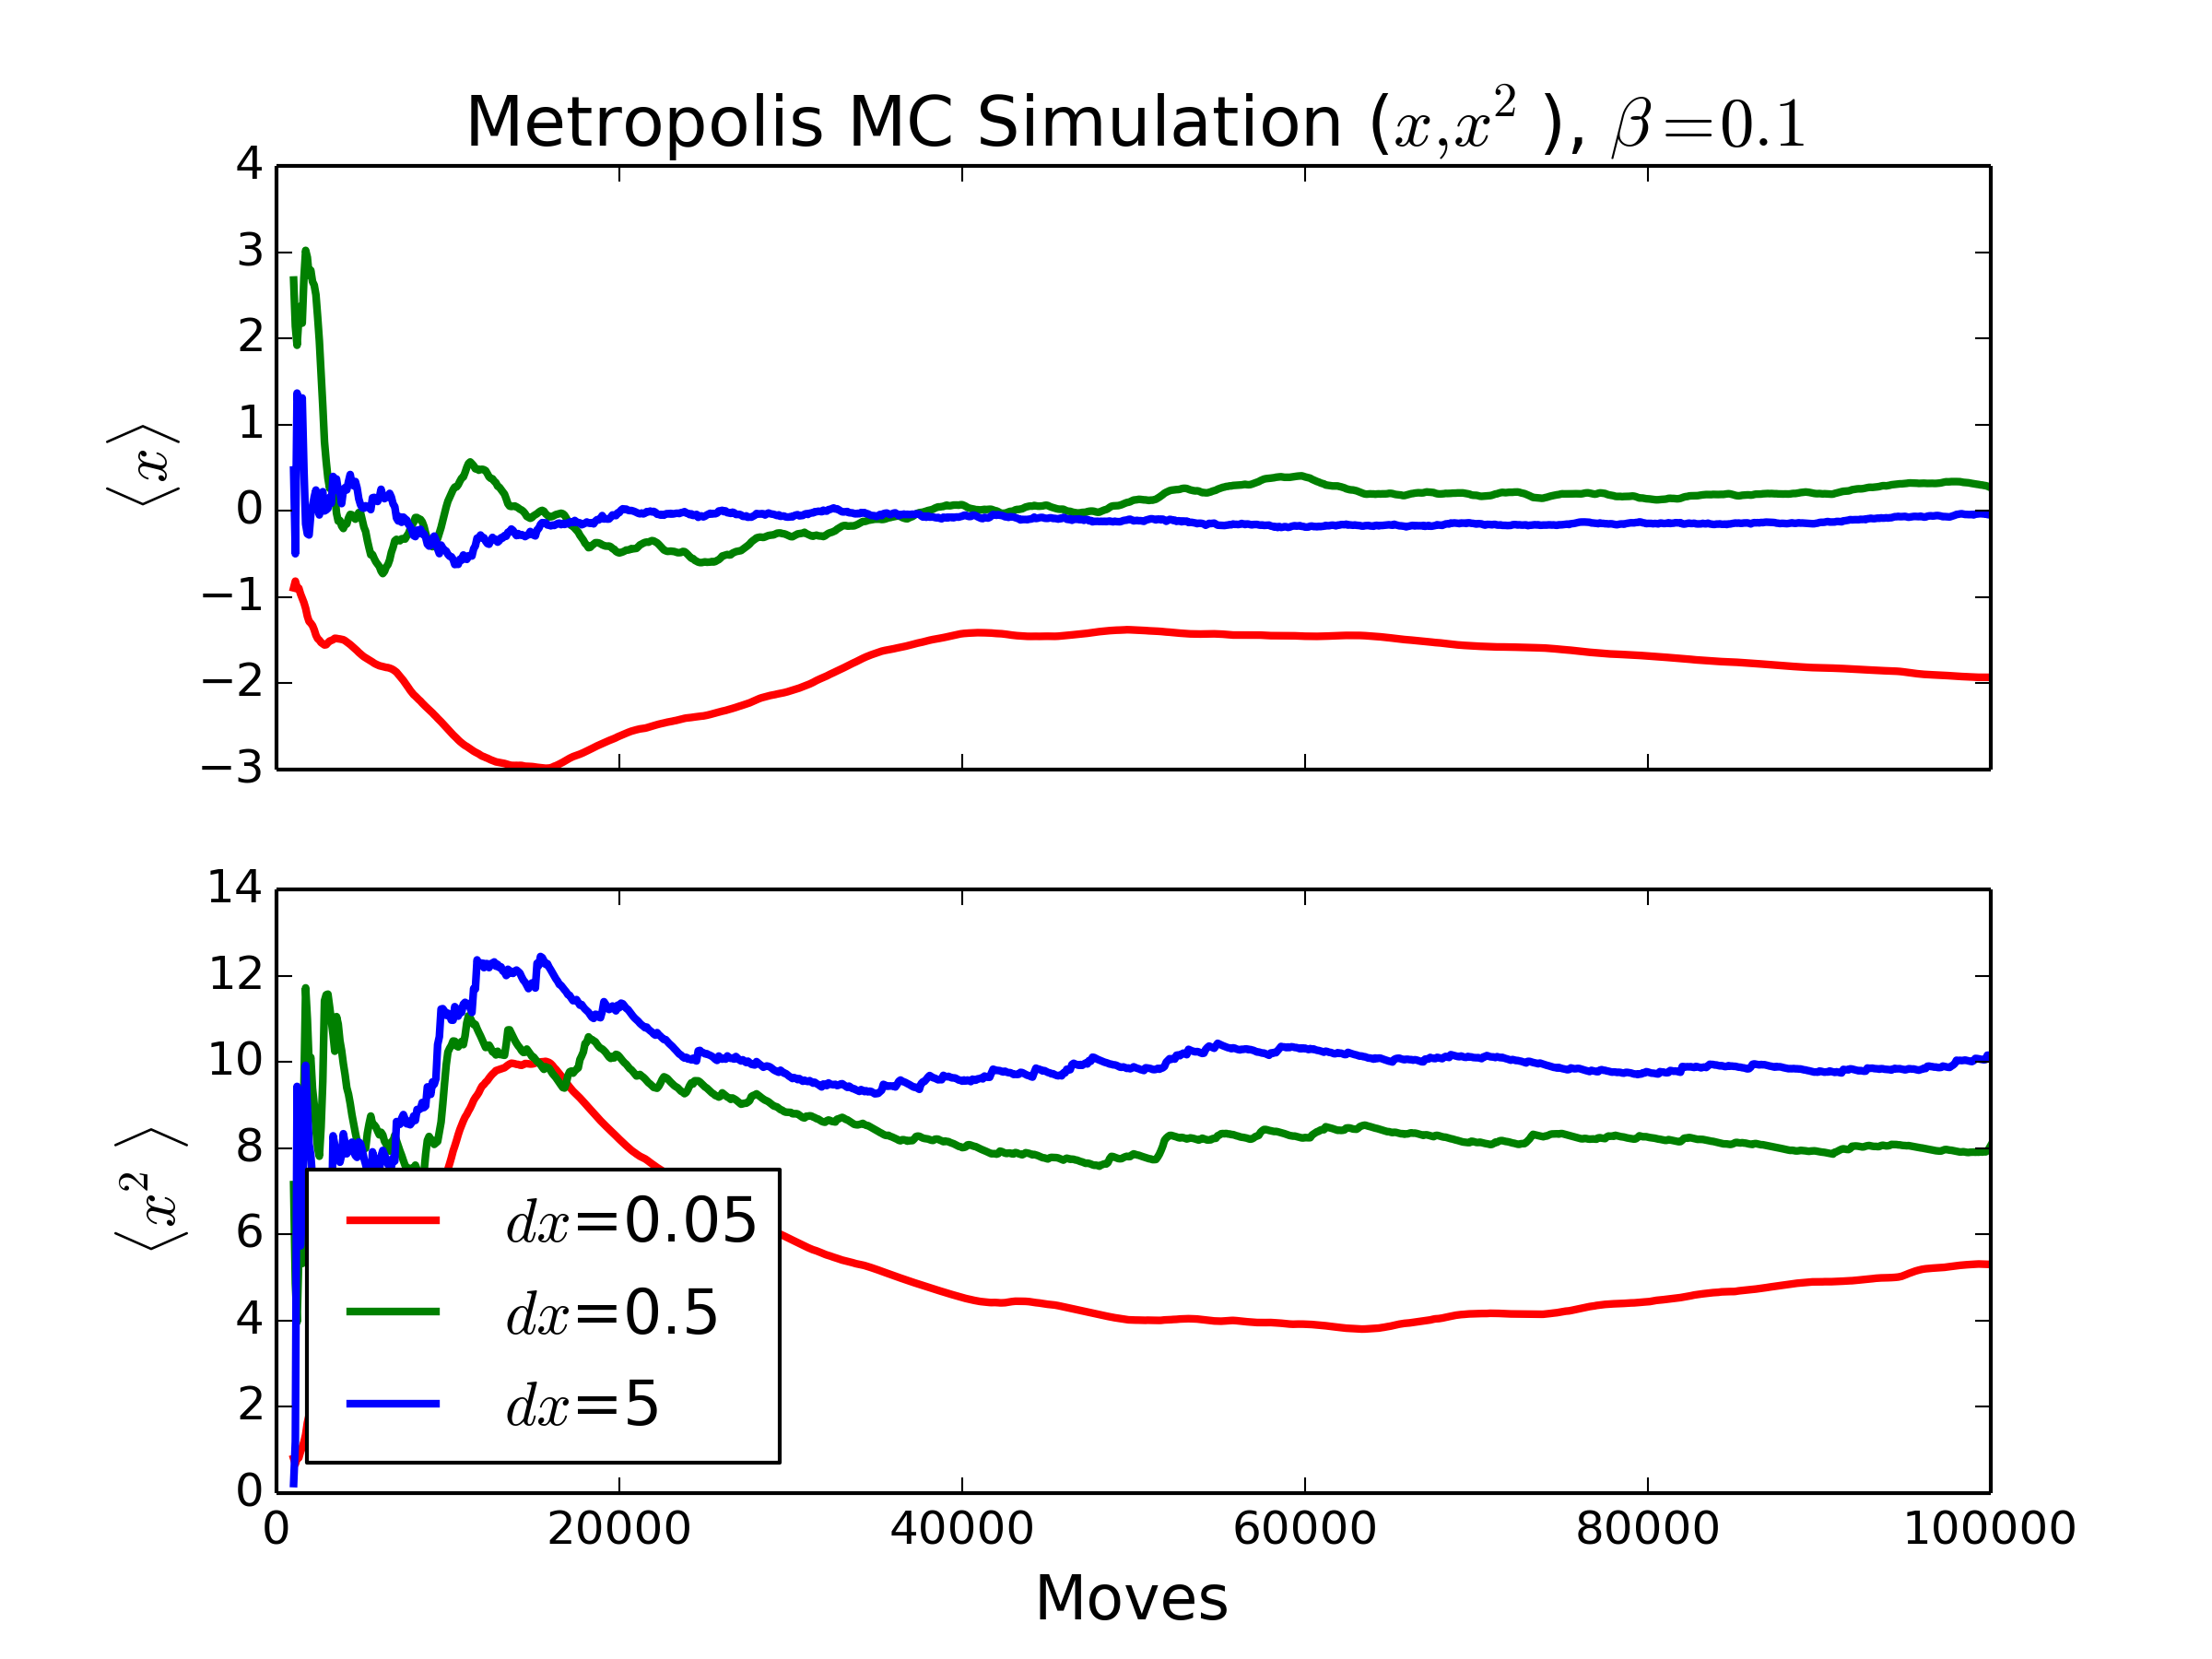
\includegraphics[width=0.49\textwidth]{./bonus/part-a-beta-0.1/Oscillator2a-x.png}\label{fig:f1}}
  \caption{Monte Carlo Simulation of oscillator at \beta=0.1}
\end{figure}

\begin{figure}[!tbp]
  \centering
\subfloat{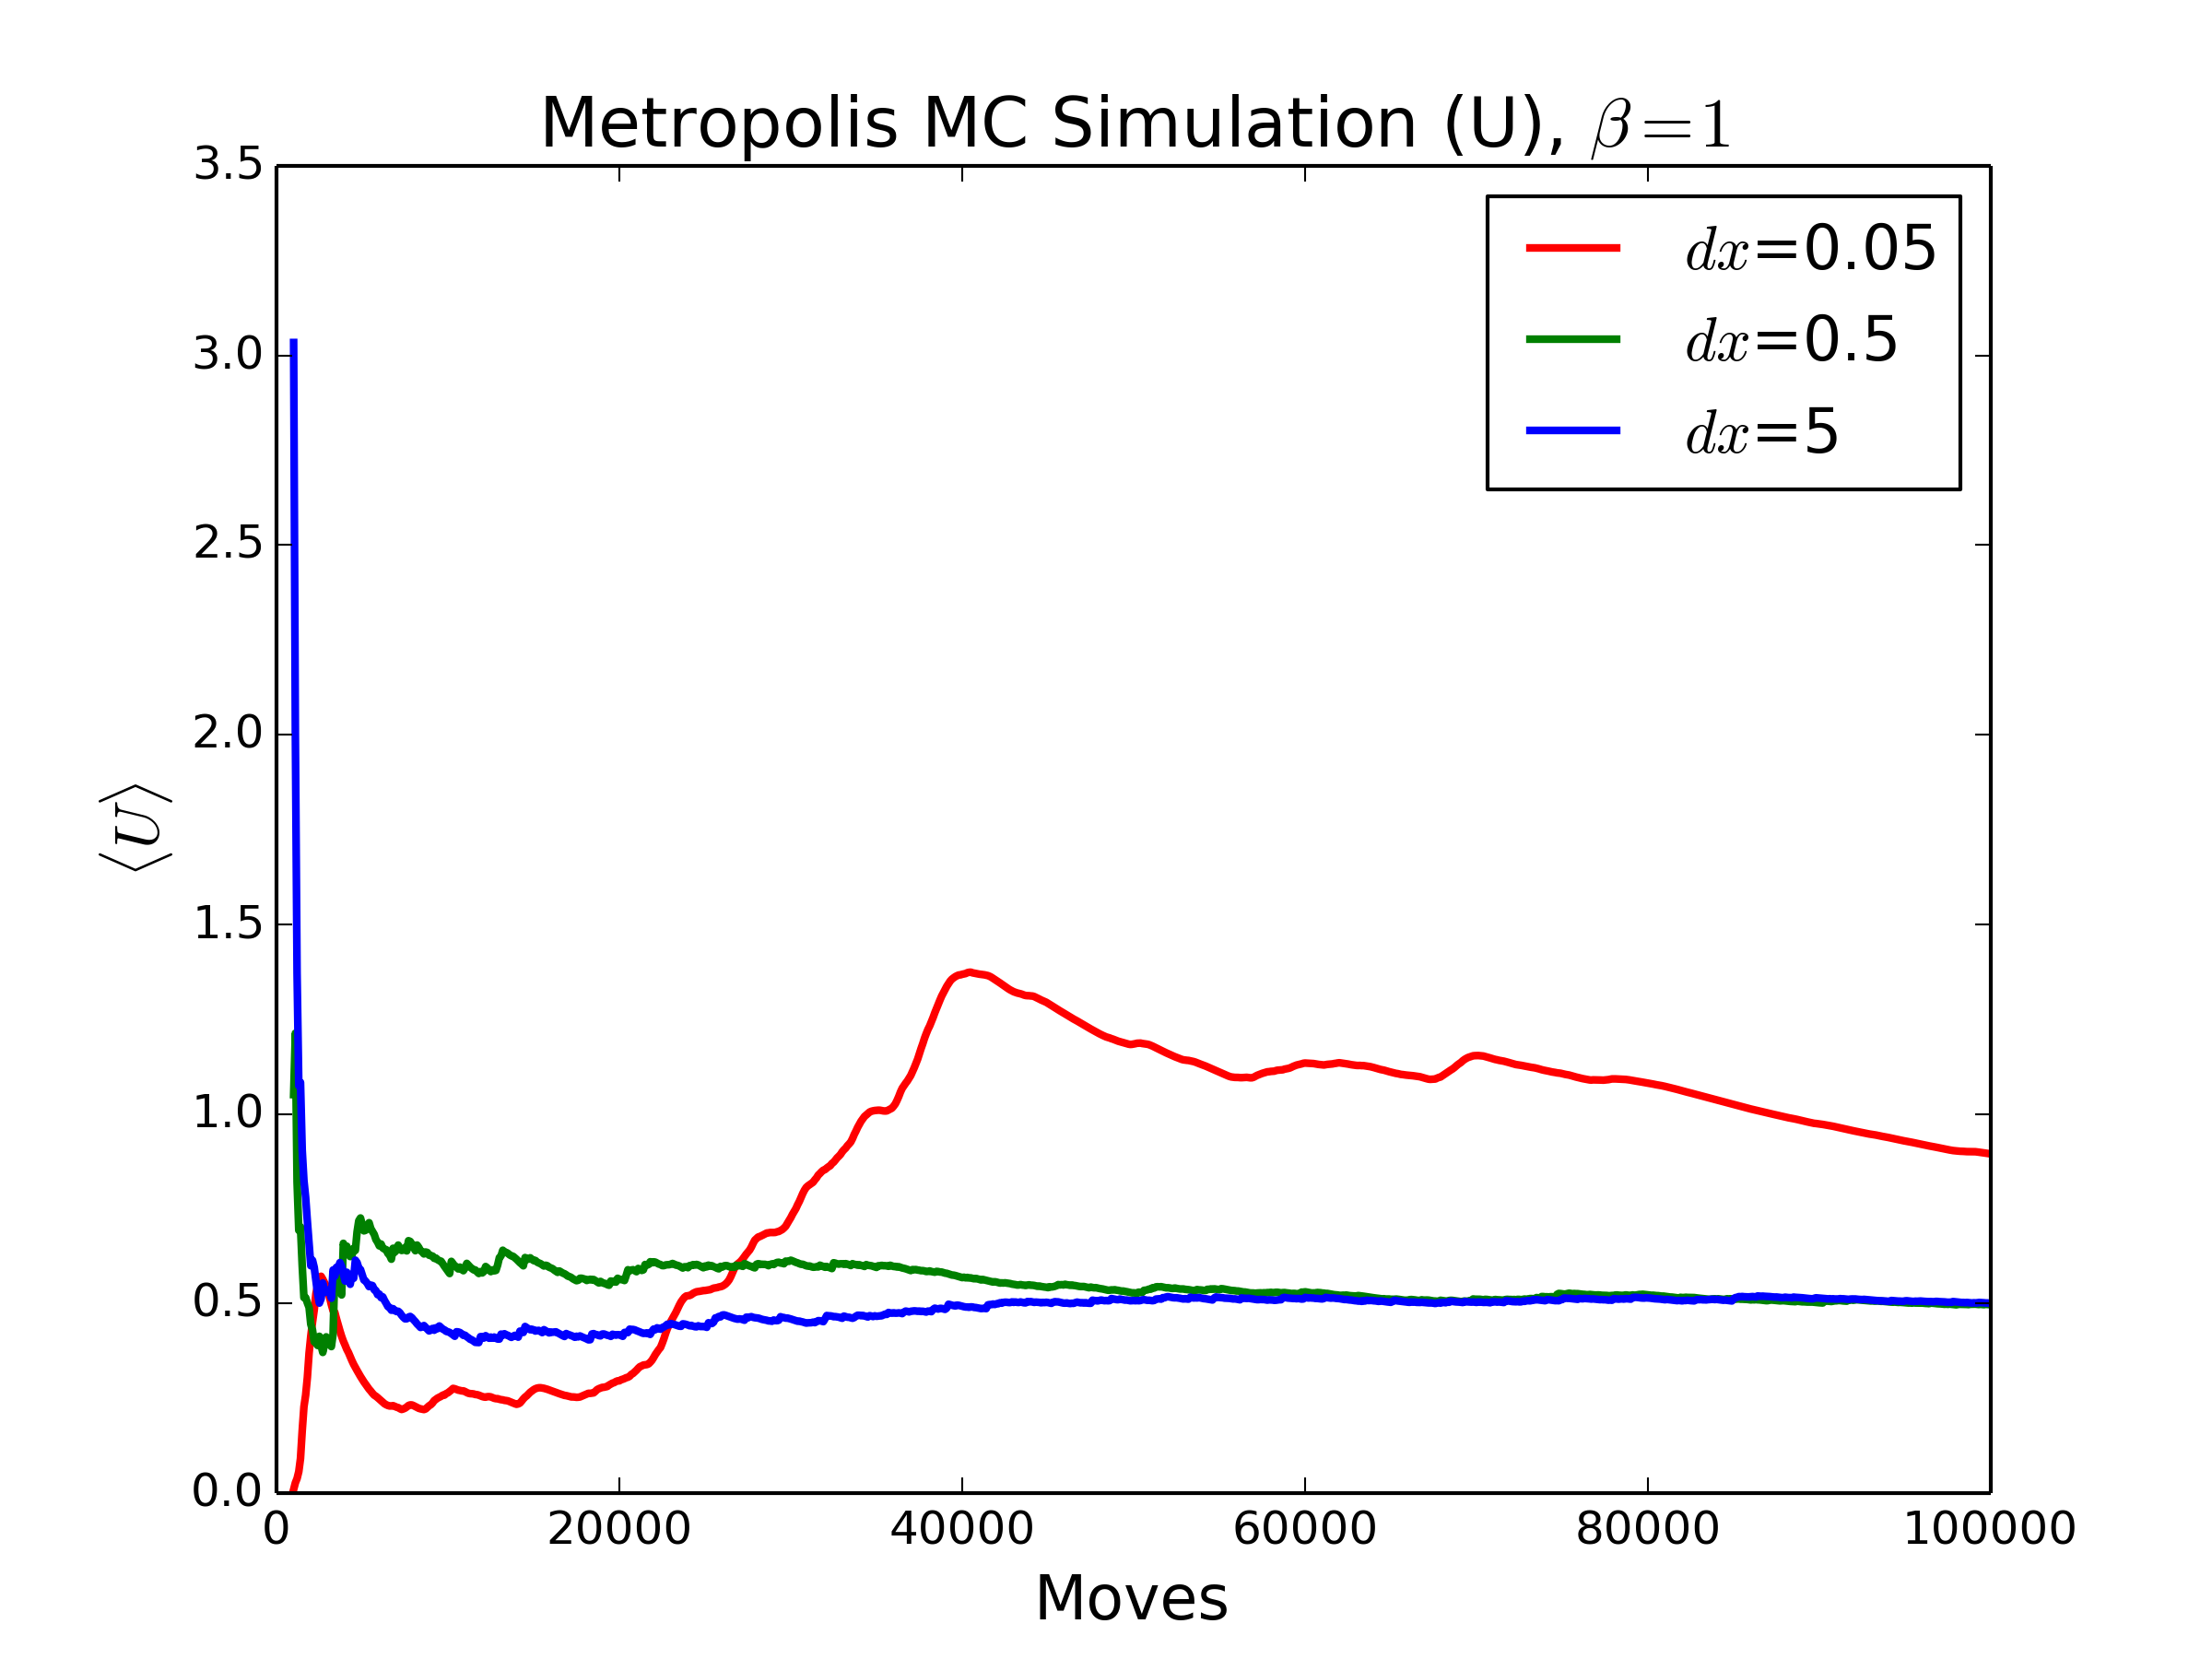
\includegraphics[width=0.49\textwidth]{./bonus/part-a-beta-1/Oscillator2a-U.png}\label{fig:f1}}
  \hfill
\subfloat{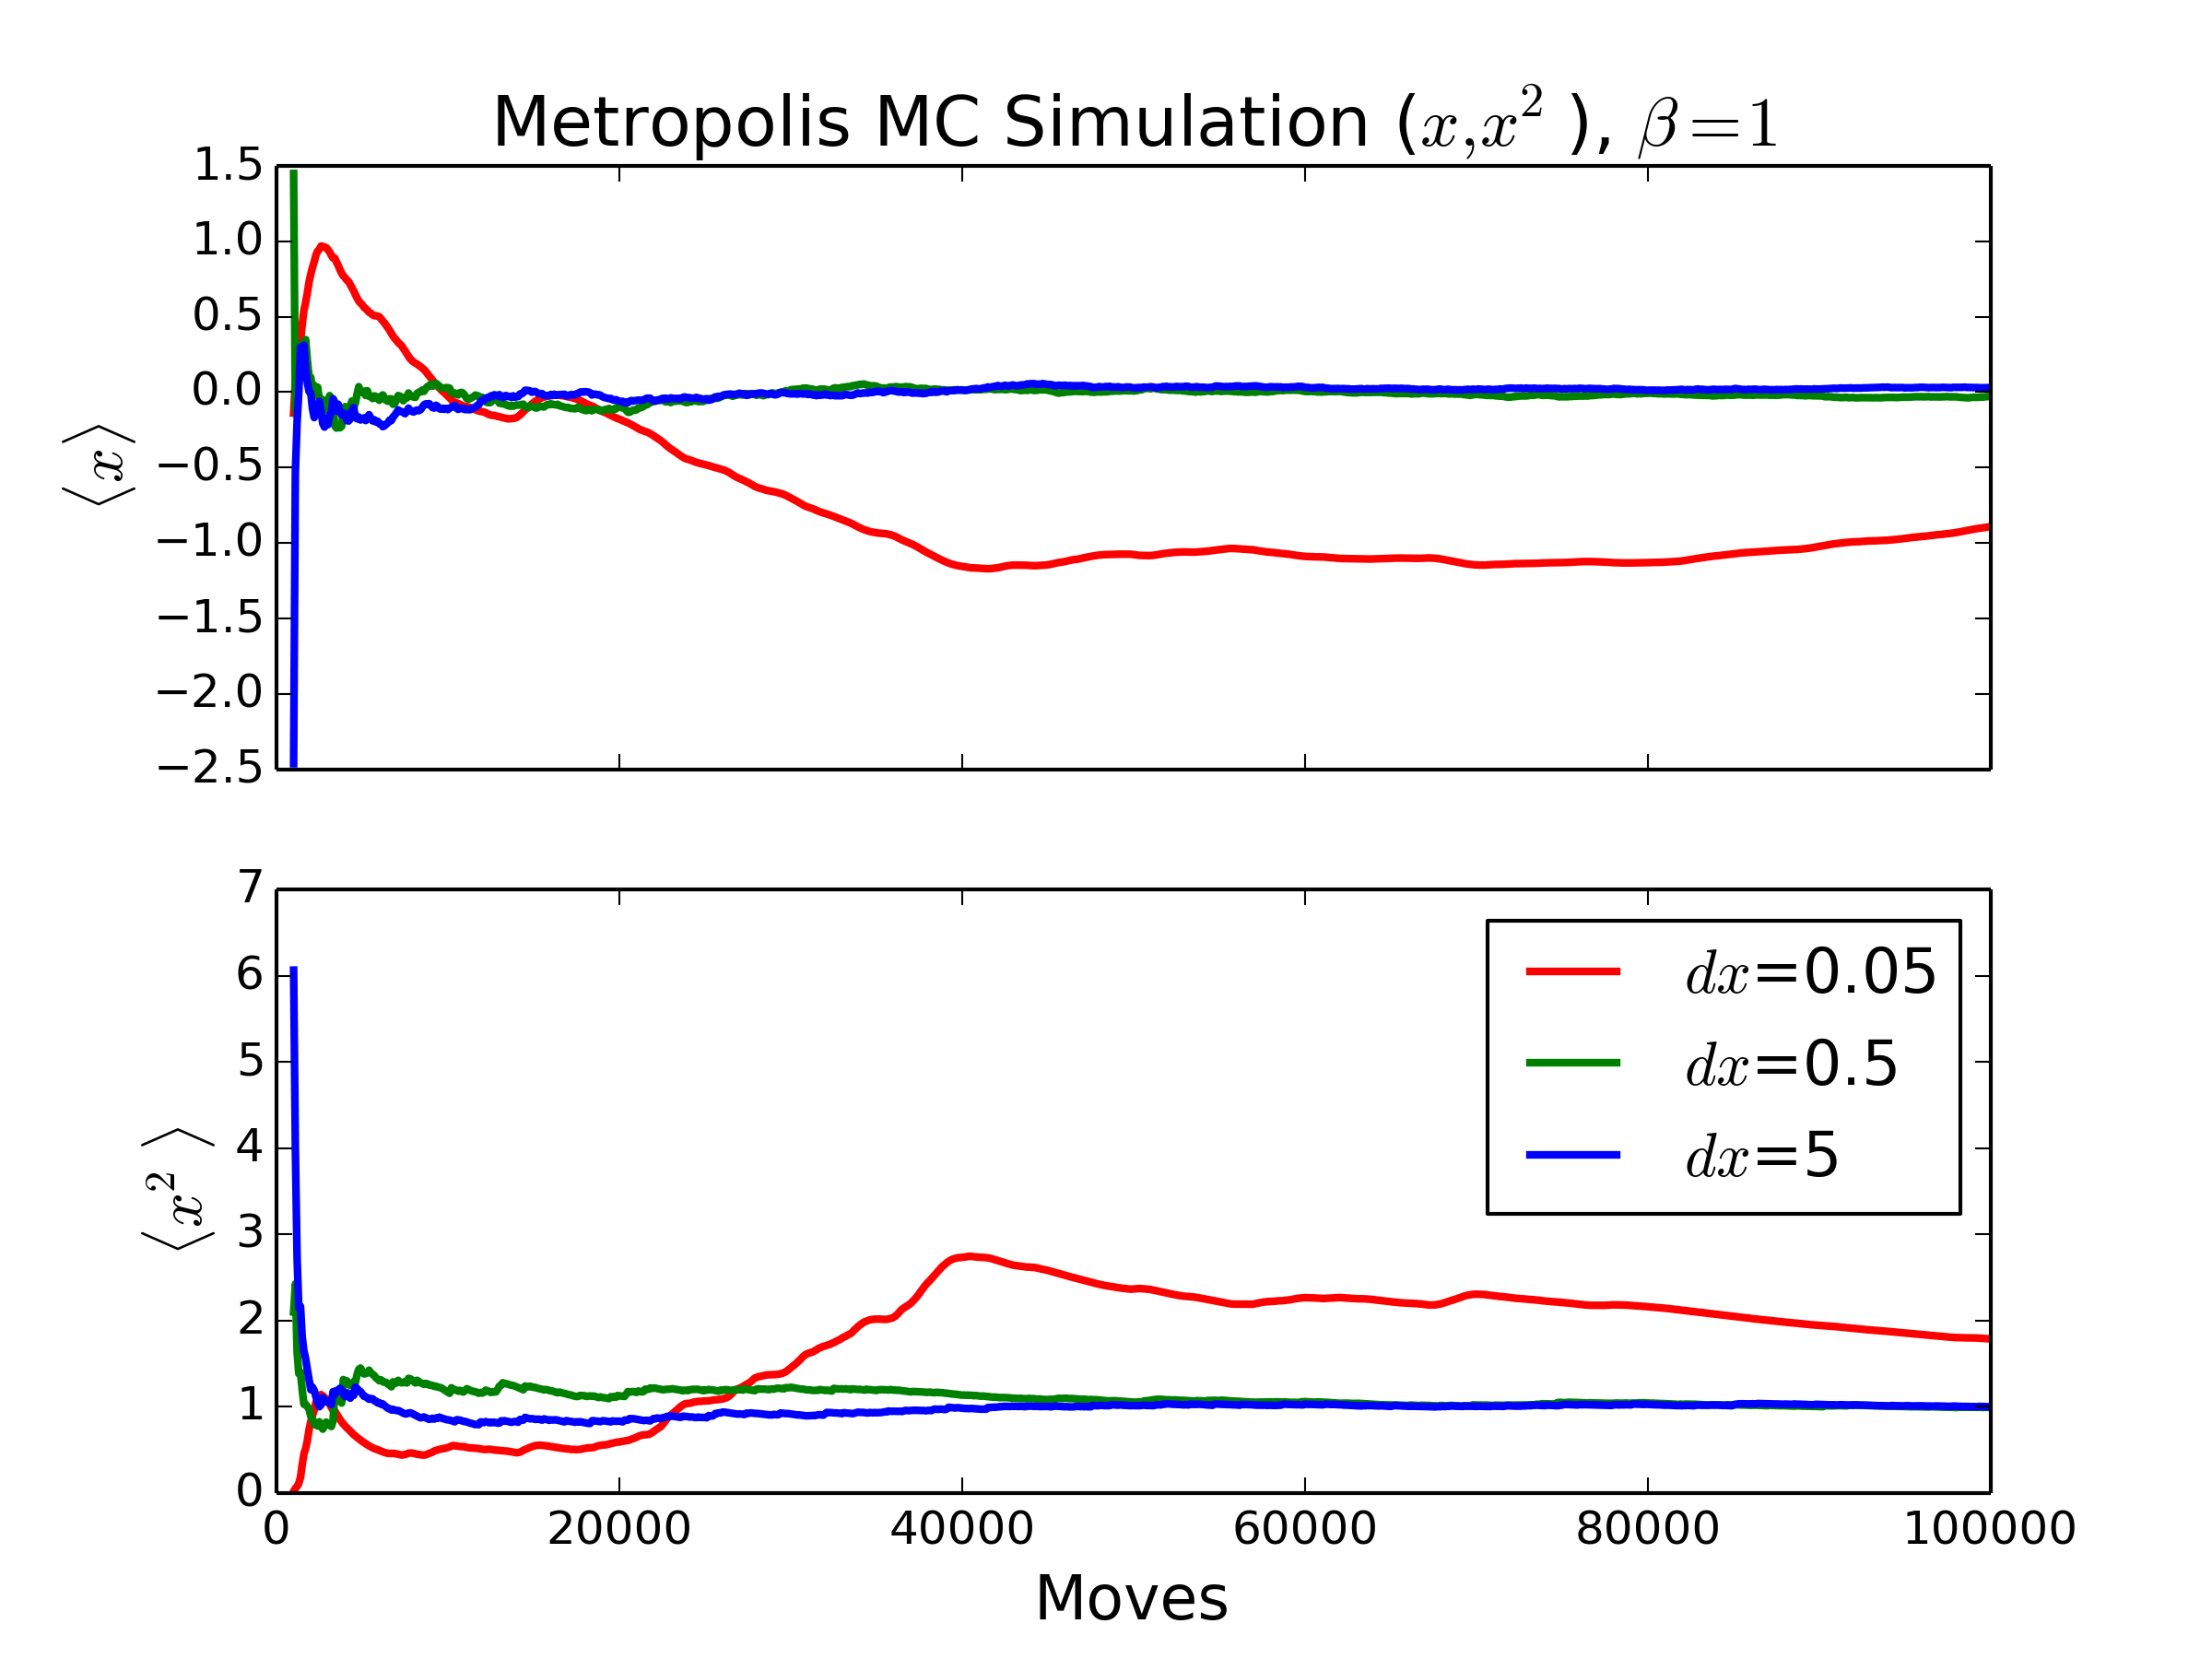
\includegraphics[width=0.49\textwidth]{./bonus/part-a-beta-1/Oscillator2a-x.png}\label{fig:f1}}
  \caption{Monte Carlo Simulation of oscillator at \beta=1}
\end{figure}

\begin{figure}[!tbp]
  \centering
\subfloat{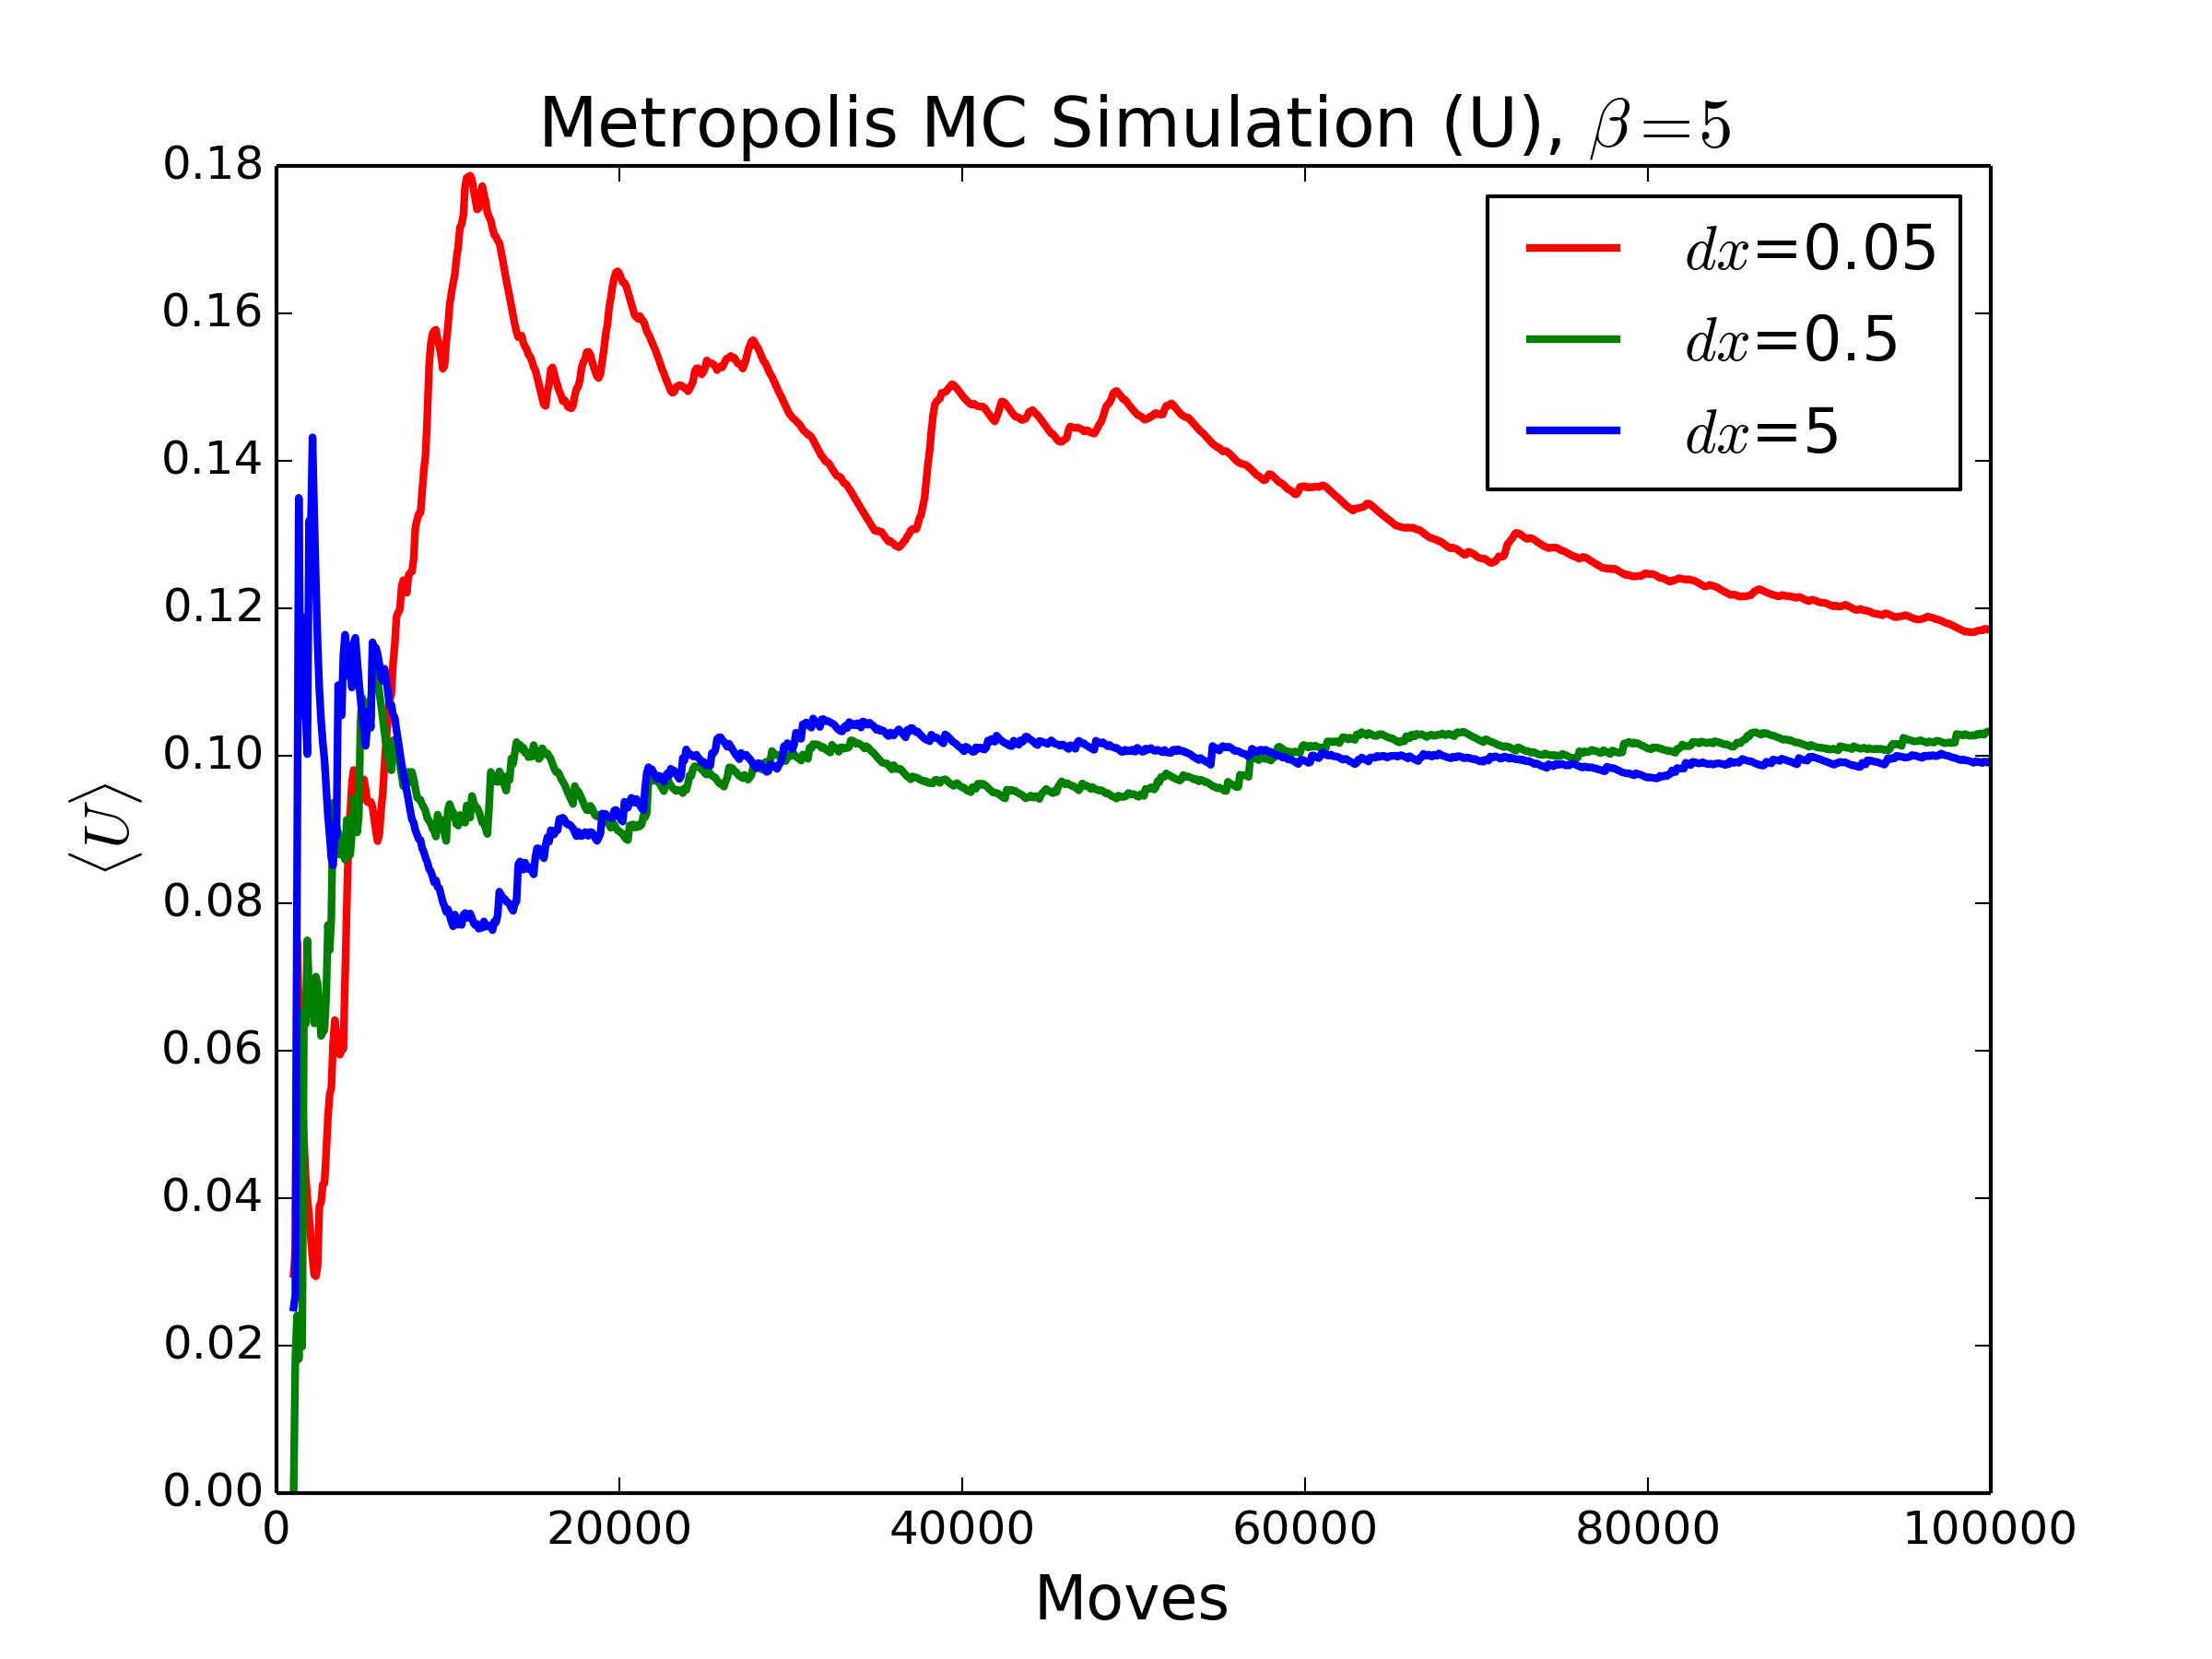
\includegraphics[width=0.49\textwidth]{./bonus/part-a-beta-5/Oscillator2a-U.png}\label{fig:f1}}
  \hfill
\subfloat{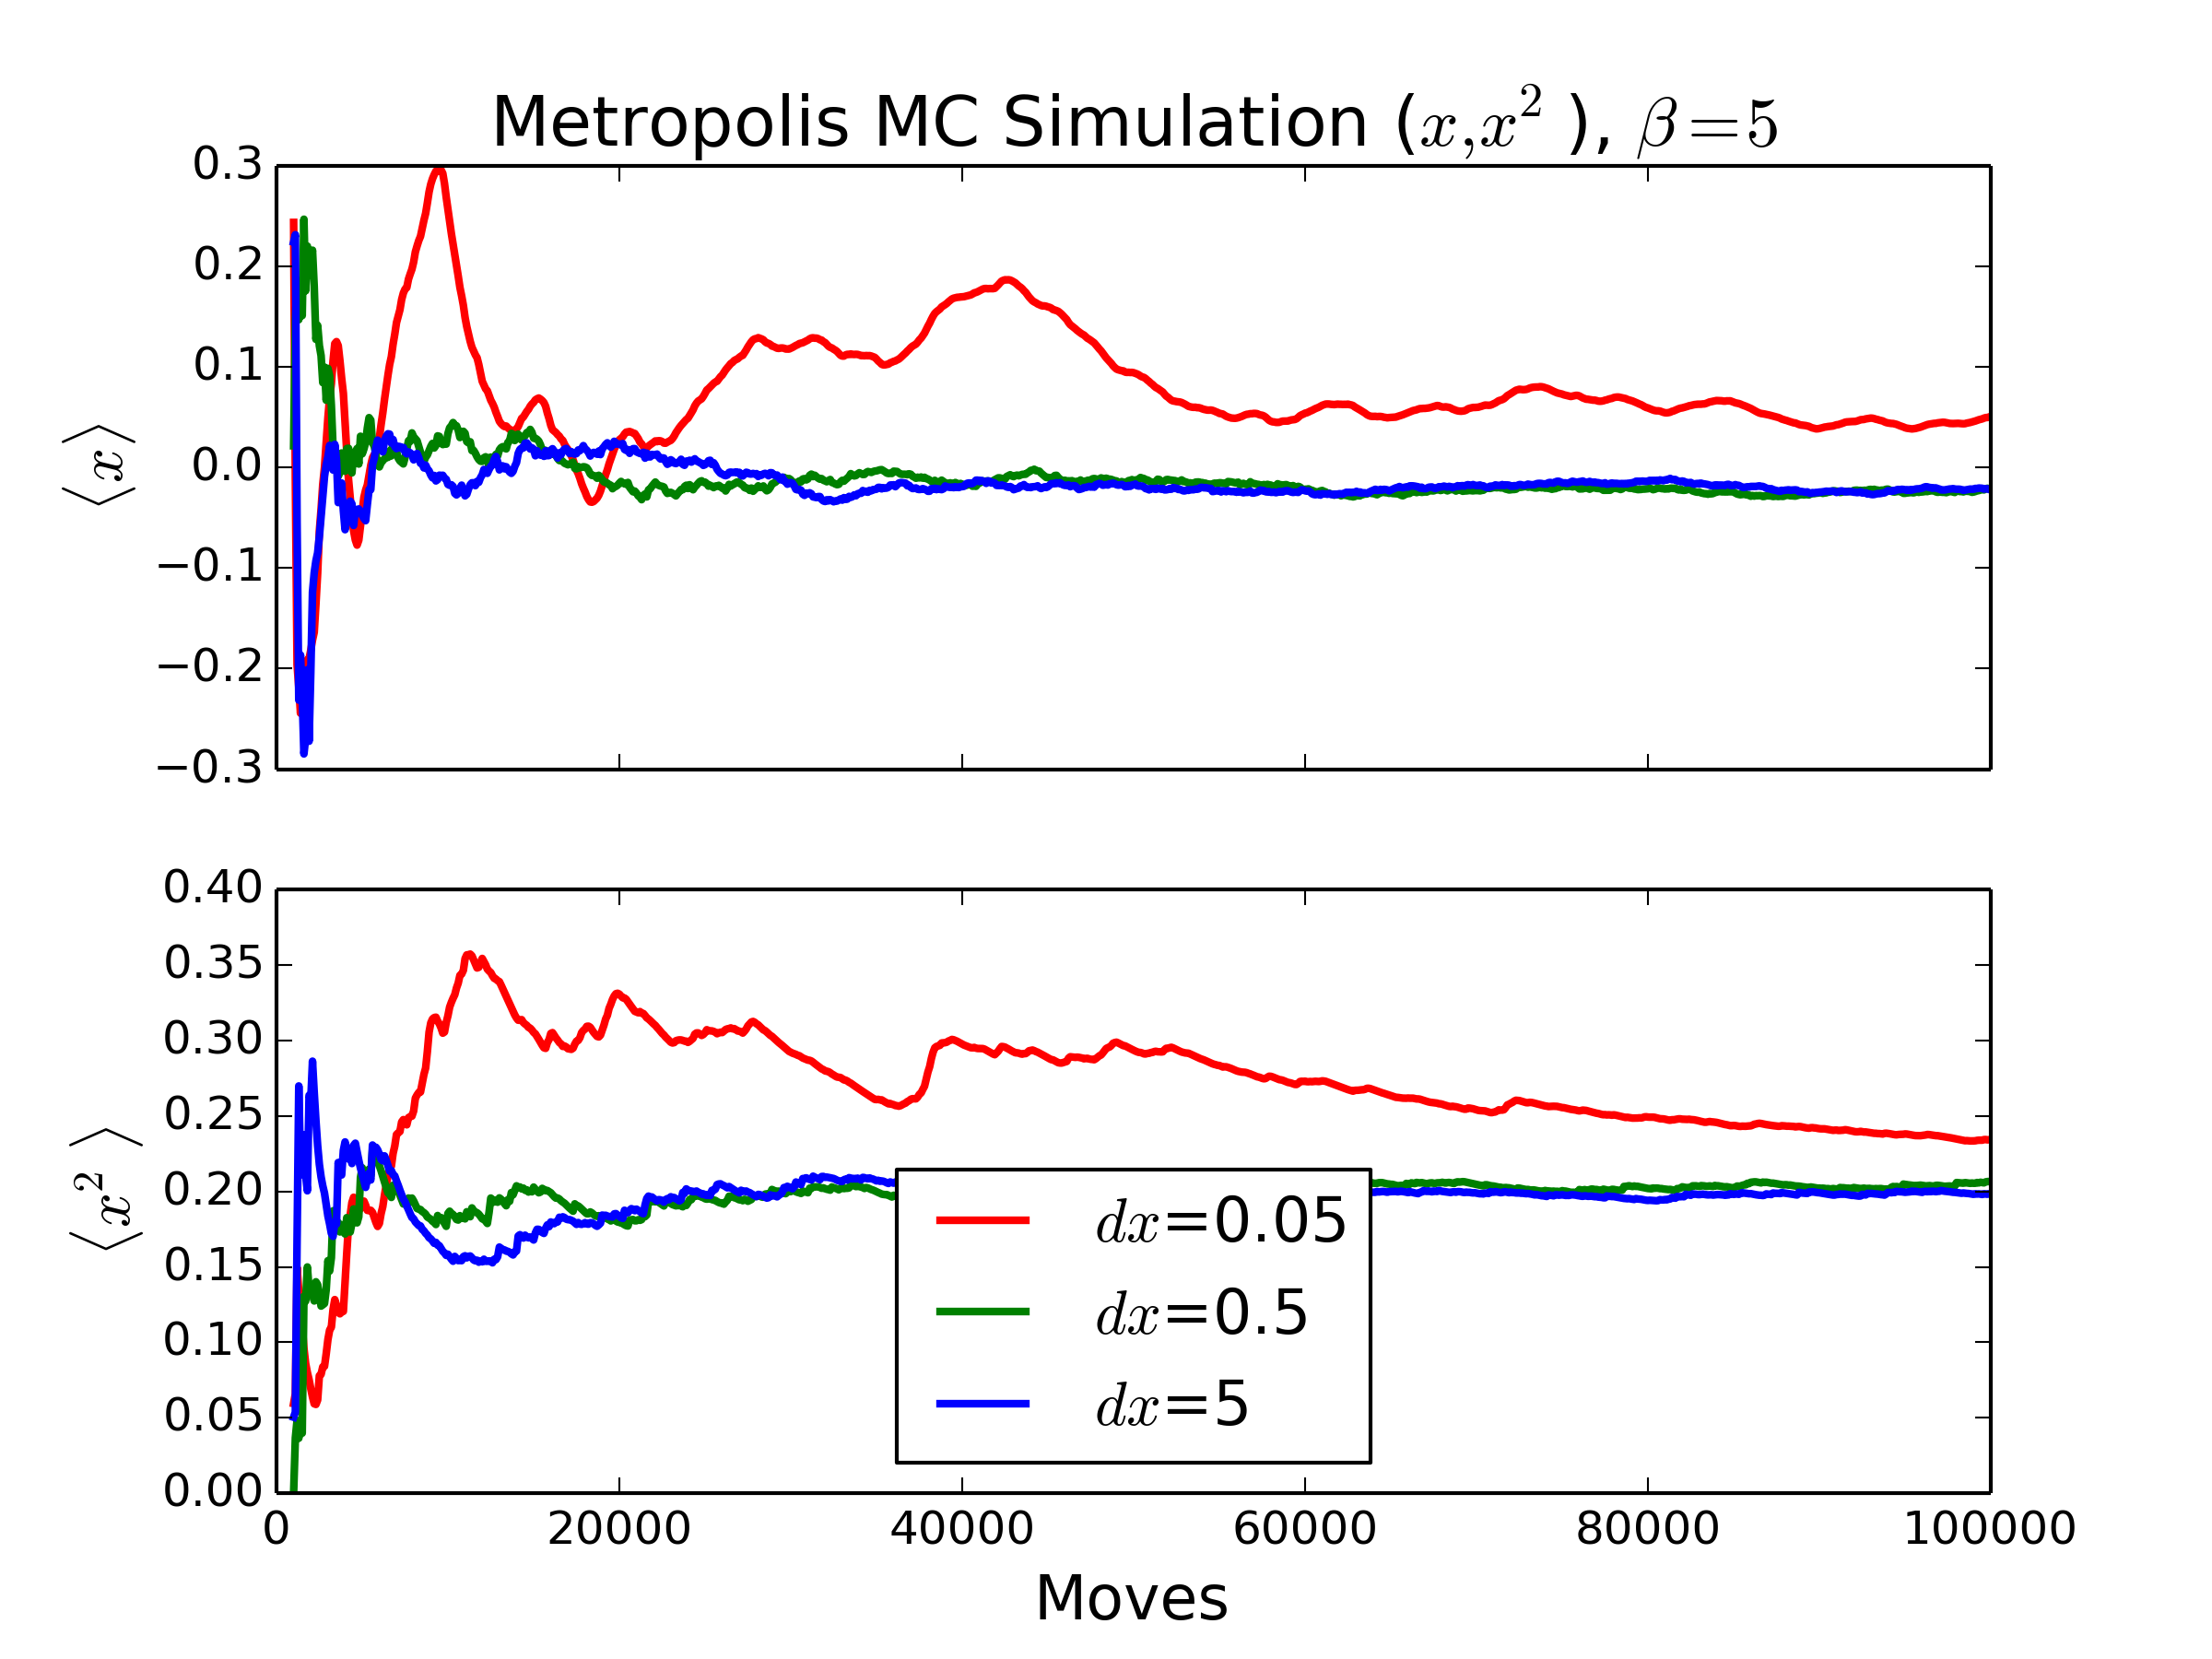
\includegraphics[width=0.49\textwidth]{./bonus/part-a-beta-5/Oscillator2a-x.png}\label{fig:f1}}
  \caption{Monte Carlo Simulation of oscillator at \beta=5}
\end{figure}

\begin{figure}[!tbp]
  \centering
\subfloat{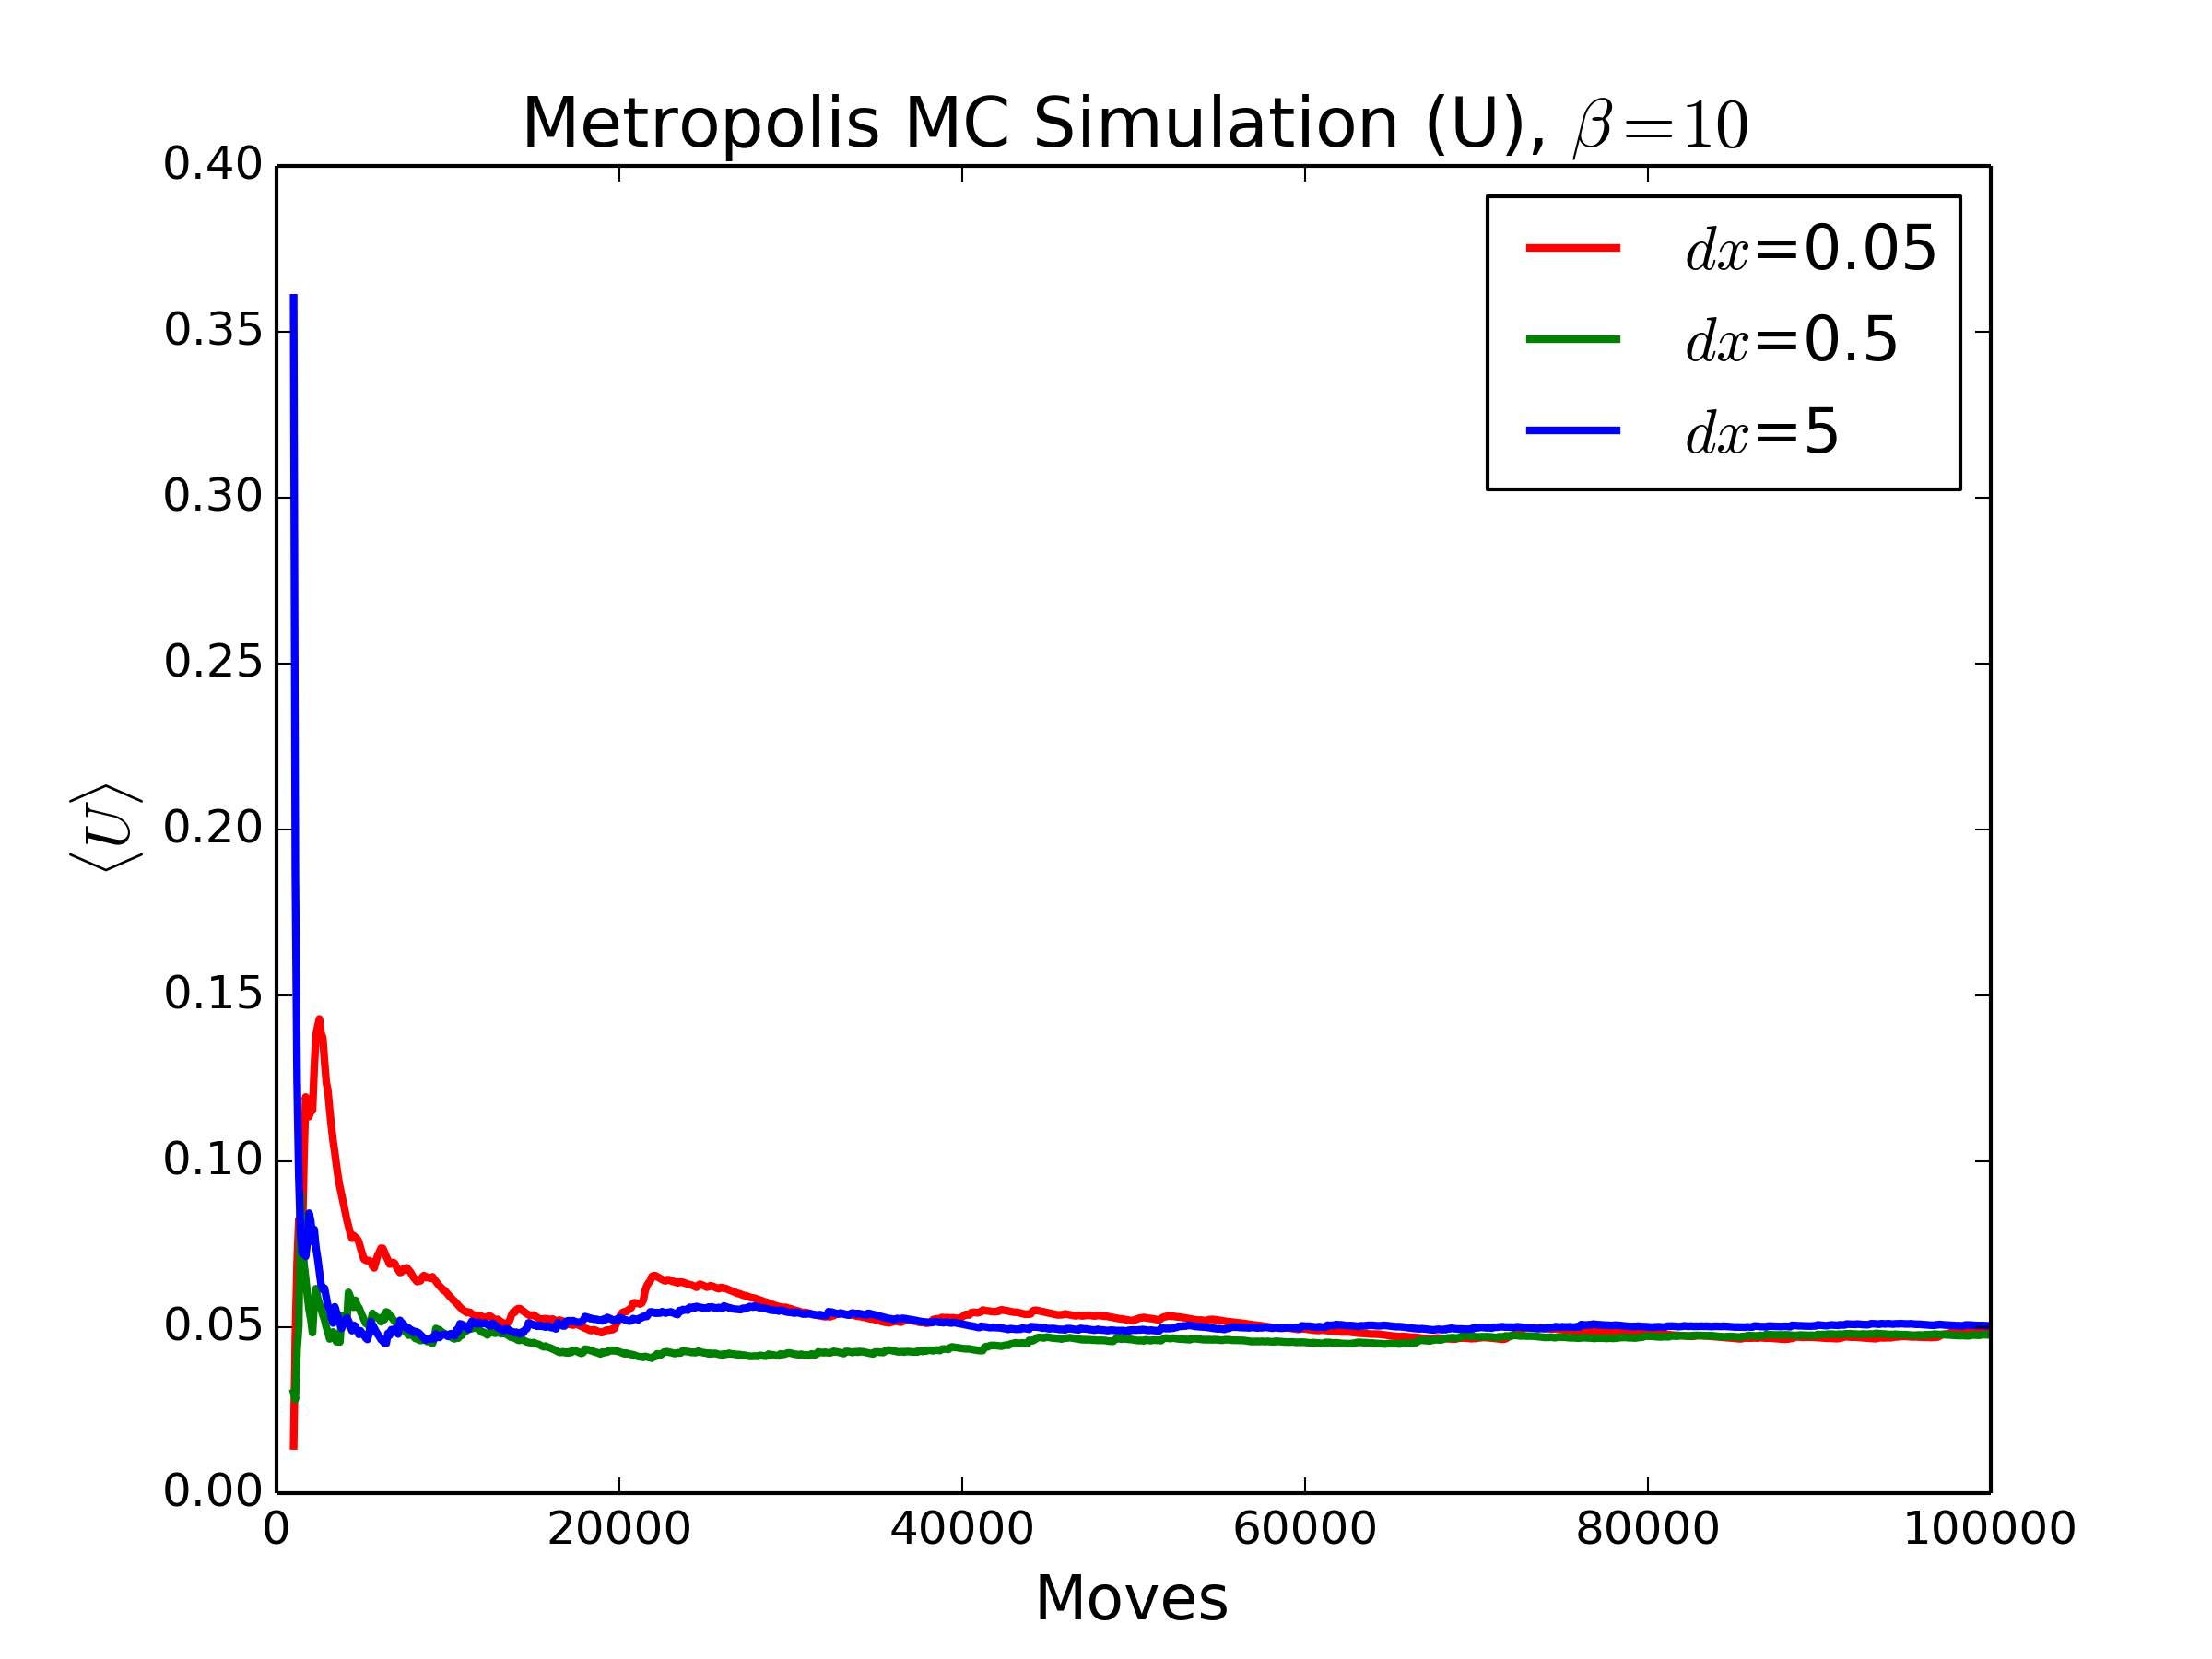
\includegraphics[width=0.49\textwidth]{./bonus/part-a-beta-10/Oscillator2a-U.png}\label{fig:f1}}
  \hfill
\subfloat{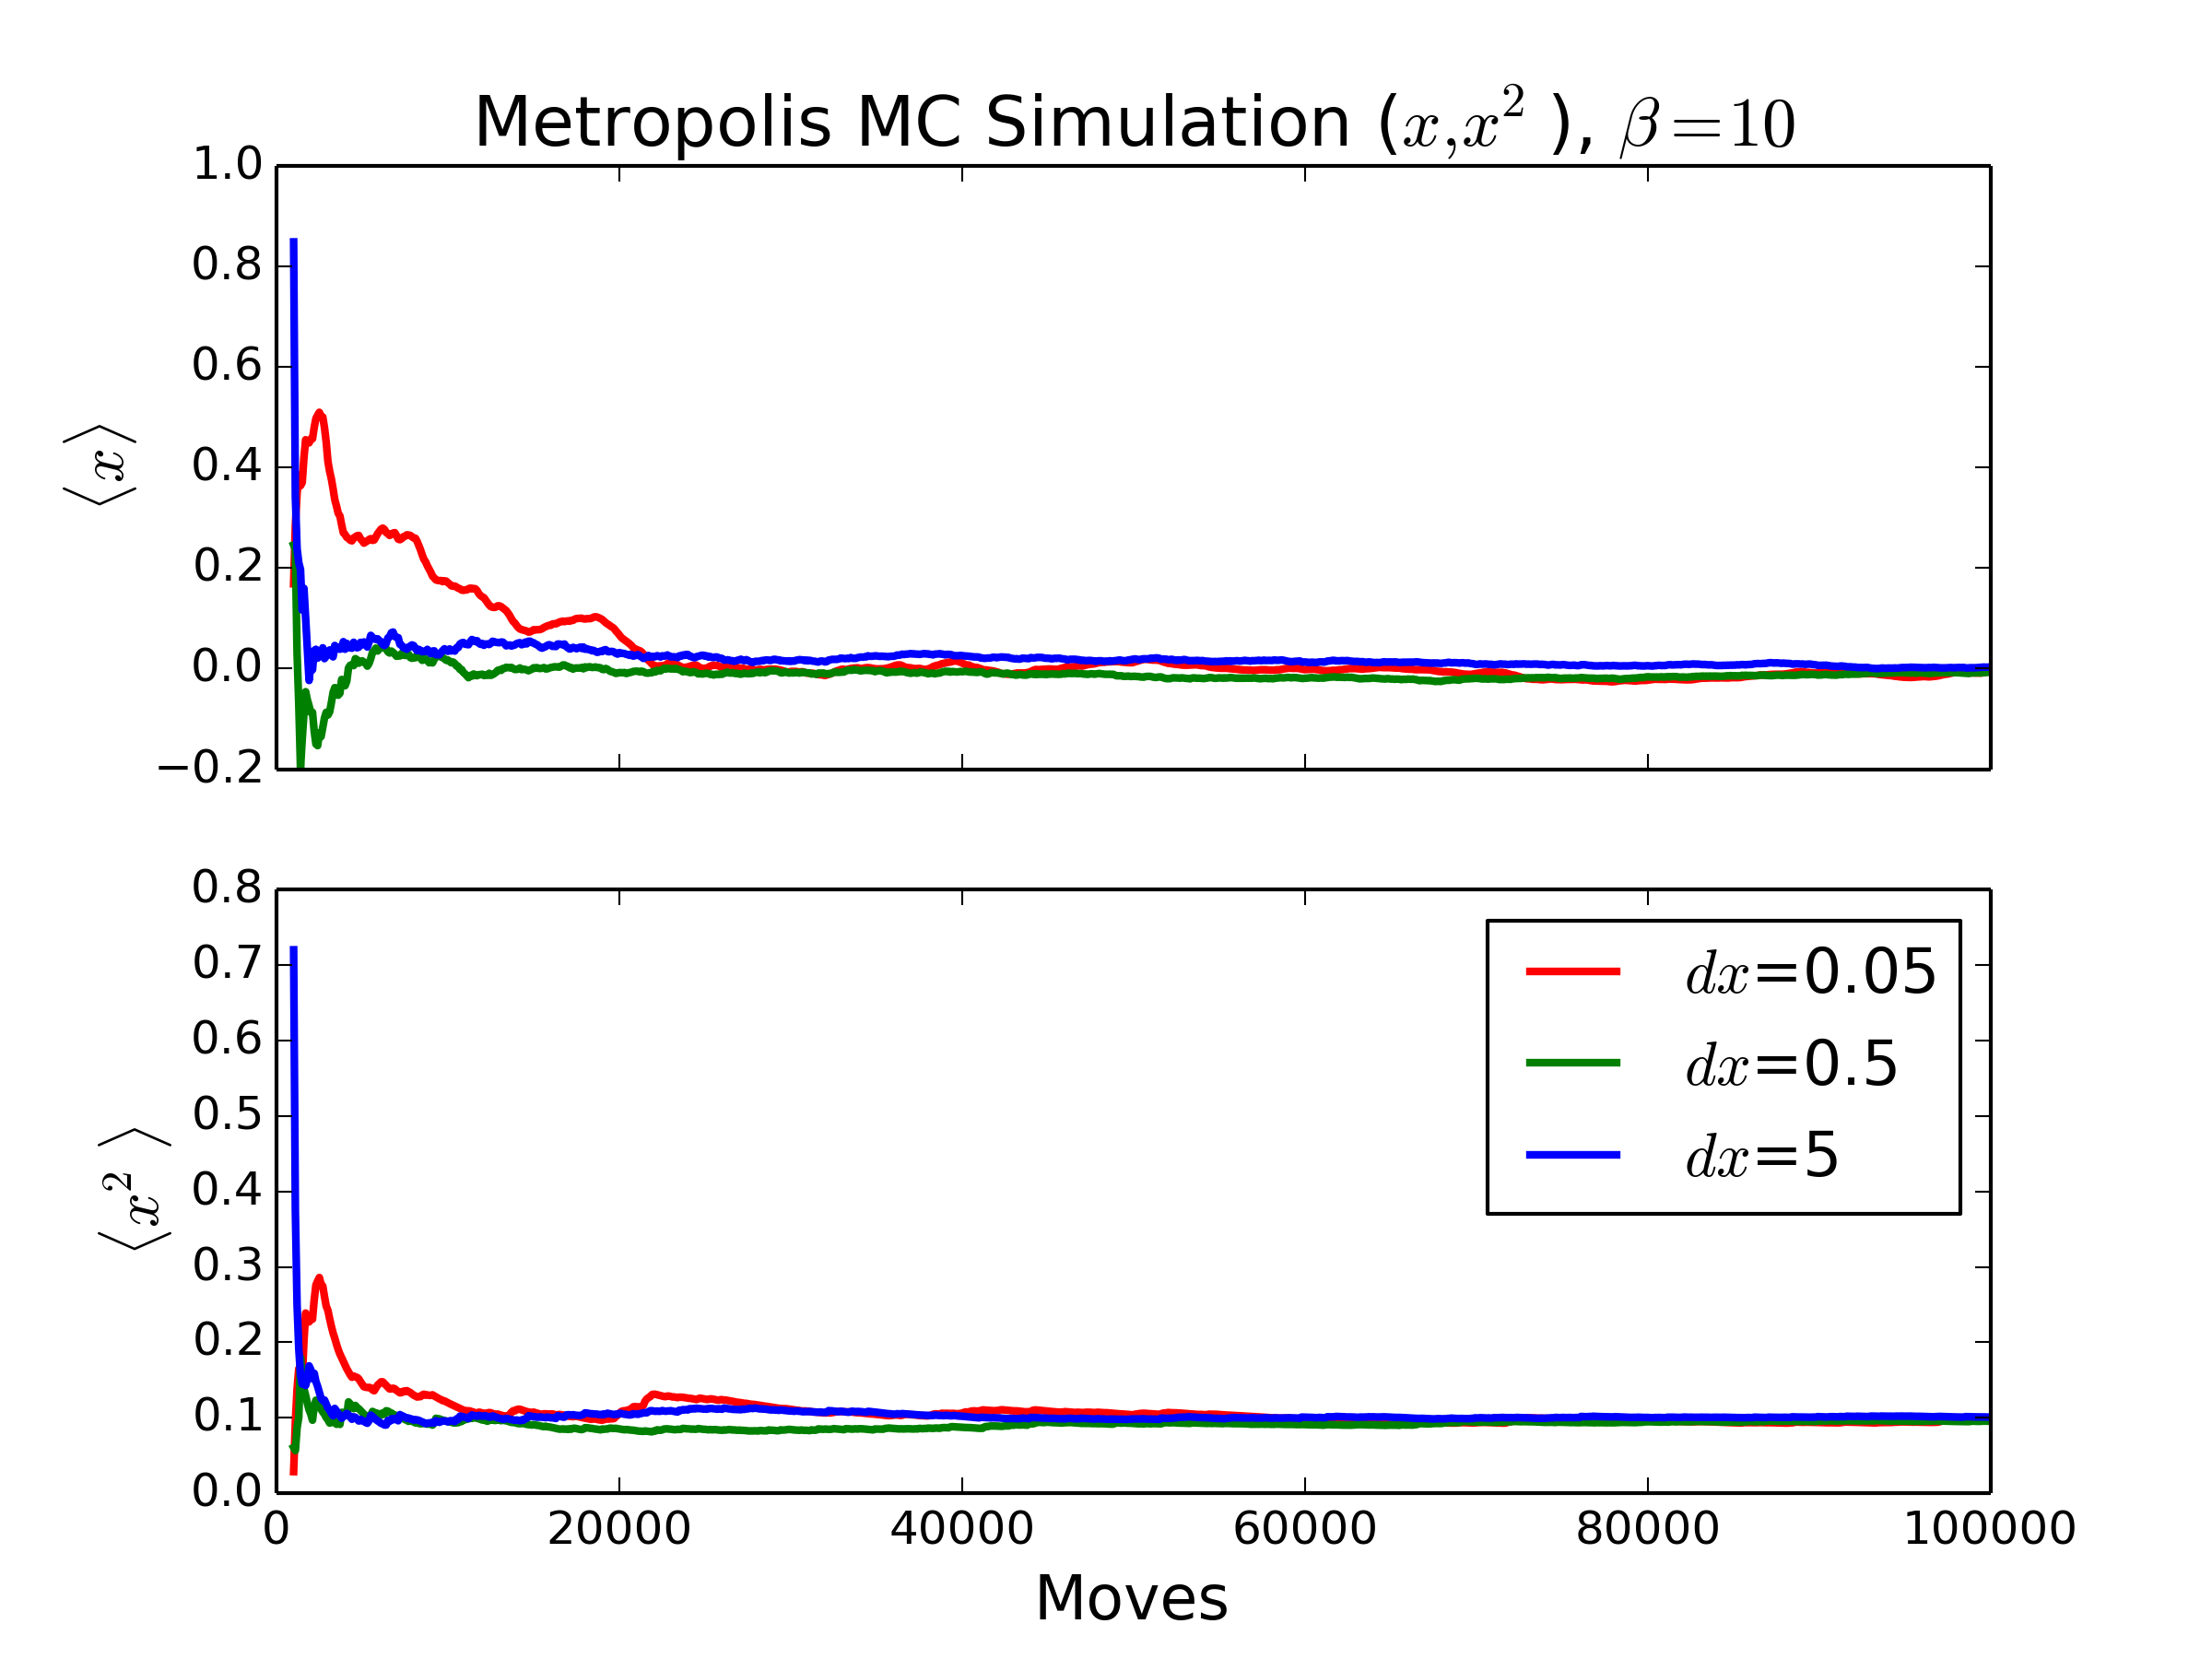
\includegraphics[width=0.49\textwidth]{./bonus/part-a-beta-10/Oscillator2a-x.png}\label{fig:f1}}
  \caption{Monte Carlo Simulation of oscillator at \beta=10}
\end{figure}

\subsection{Detailed Balance}
\label{sec-3-1}
For the detailed balance to obey, the rate to come to the 'new' configuration from 'old' configuration equals to that of from 'old' configuration to 'new' configuration.

\begin{equation}
p_{new} P(old \rightarrow new) = p_{old} P(new \rightarrow old)
\end{equation}

Lets say that $P(old \rightarrow new)$ can be written as $acc(old \rightarrow new) \alpha(old \rightarrow new)$,  hence

\begin{equation}
\frac{acc(old \rightarrow new)\alpha(old \rightarrow new)}{acc(new \rightarrow old)\alpha(new \rightarrow old)} = \frac{P(new)}{P(old)}
\end{equation}

Hence the accpetance probability condition from old configuration to new configuration can be written as,
\begin{equation}
acc(old \rightarrow new) = \frac{P(new)}{P(old)} \frac{\alpha(new \rightarrow old)}{\alpha(old \rightarrow new)} acc(new \rightarrow old)
\end{equation}

This would give us the acceptance probability to go from old state to new state as follows : 

\begin{equation}
\boxed{acc(old \rightarrow new) = \frac{exp(-\beta \delta E/2)}{exp(-\beta \delta E/2) + exp(\beta \delta E/2)} acc(new \rightarrow old)}
\end{equation}

By exploring the acceptance probability from new state to old state would give us :
\begin{equation}
\boxed{acc(new \rightarrow old) = \frac{exp( \beta \delta E/2)}{exp(\beta \delta E/2) + exp(-\beta \delta E/2)} acc(old \rightarrow new)}
\end{equation}

where, $\delta E = U(new) - U(old)$, which takes a negative sign in vice-versa.
% Emacs 24.4.1 (Org mode 8.2.10)
\end{document}